\documentclass[a4paper,12pt,oneside]{ThesisStyle}

%\usepackage[style=verbose]{biblatex}

\usepackage{listings}
\usepackage{color}
\usepackage[utf8]{vietnam}
%\usepackage[monochrome]{color} %enable to make black-while print version
\usepackage{arial}	% same Time New Roma
\usepackage{titlesec}
\usepackage{subcaption}
\usepackage{amsmath}
\titleformat
{\chapter} % command
[display] % shape
{\bfseries\LARGE} % format
{\Large{Chương} \ \thechapter} % label
{0.5ex} % sep
{
    \rule{\textwidth}{1pt}
    \vspace{1ex}
    \centering
} % before-code
[
\vspace{-0.5ex}%
\rule{\textwidth}{0.3pt}
] % after-code


\titlespacing*{\chapter}{0pt}{-1cm}{1cm}


%\end trong add

\usepackage{tabularx}
\usepackage{multirow}
\usepackage{pdf14}
\usepackage{pgfplots}
\usetikzlibrary{calc}
\usepackage{booktabs}
\usepackage{array}
\usepackage{tikz}
\usepackage{amsmath,amssymb}             % AMS Math
\usepackage[left=3cm,right=2cm,top=2cm,bottom=2cm,includefoot,includehead,headheight=13.6pt]{geometry}

\usepackage{floatrow}
\floatsetup[table]{capposition=top}
\usepackage{multirow}
\usepackage[english]{babel}
\usepackage[format=plain,indention=1em]{caption}
\usepackage{float}
\usepackage{booktabs}
\newcommand\abs[1]{\left|#1\right|}

\renewcommand{\baselinestretch}{1.05}

% Table of contents for each chapter

\usepackage[nottoc, notlof, notlot]{tocbibind}
\usepackage{minitoc}
\setcounter{minitocdepth}{2}
\mtcindent=15pt
% Use \minitoc where to put a table of contents

\usepackage{aecompl}

% Glossary / list of abbreviations

\usepackage[intoc]{nomencl}
\renewcommand{\nomname}{List of Abbreviations}

\makenomenclature

% My pdf code

\usepackage{ifpdf}

\ifpdf
  %\usepackage[pdftex]{graphicx}
  \DeclareGraphicsExtensions{.jpg}
  \usepackage[a4paper,pagebackref,hyperindex=true]{hyperref}
\else
  \usepackage{graphicx}
  \DeclareGraphicsExtensions{.ps,.eps}
  \usepackage[a4paper,dvipdfm,pagebackref,hyperindex=true]{hyperref}
\fi

\graphicspath{{.}{images/}}

% nicer backref links
\renewcommand*{\backref}[1]{}
\renewcommand*{\backrefalt}[4]{%
\ifcase #1 %
(Not cited.)%
\or
(Cited on page~#2.)%
\else
(Cited on pages~#2.)%
\fi}
\renewcommand*{\backrefsep}{, }
\renewcommand*{\backreftwosep}{ and~}
\renewcommand*{\backreflastsep}{ and~}

% Links in pdf
\usepackage{color}
\definecolor{linkcol}{rgb}{0,0,0.4} 
\definecolor{citecol}{rgb}{0.5,0,0} 
\definecolor{gray}{rgb}{0.4,0.4,0.4}
\definecolor{darkblue}{rgb}{0.0,0.0,0.6}
\definecolor{cyan}{rgb}{0.0,0.6,0.6}

\lstset{
  basicstyle=\ttfamily,
  columns=fullflexible,
  showstringspaces=false,
  commentstyle=\color{gray}\upshape
}

\lstdefinelanguage{XML}
{
  morestring=[b]",
  morestring=[s]{>}{<},
  morecomment=[s]{<?}{?>},
  stringstyle=\color{black},
  identifierstyle=\color{darkblue},
  keywordstyle=\color{cyan},
  morekeywords={annotation, folder, filename, path, source, size, width, height, depth, segmented, object, name, pose, truncated, difficult, bndbox, xmin, ymin, xmax, ymax, database}% list your attributes here
}

% Change this to change the informations included in the pdf file

% See hyperref documentation for information on those parameters

\hypersetup
{
bookmarksopen=true,
pdftitle="Design and Use of Anatomical Atlases for Radiotherapy",
pdfauthor="Olivier COMMOWICK", 
pdfsubject="Creation of atlases and atlas based segmentation", %subject of the document
%pdftoolbar=false, % toolbar hidden
pdfmenubar=true, %menubar shown
pdfhighlight=/O, %effect of clicking on a link
colorlinks=true, %couleurs sur les liens hypertextes
pdfpagemode=None, %aucun mode de page
pdfpagelayout=SinglePage, %ouverture en simple page
pdffitwindow=true, %pages ouvertes entierement dans toute la fenetre
linkcolor=linkcol, %couleur des liens hypertextes internes
citecolor=citecol, %couleur des liens pour les citations
urlcolor=linkcol %couleur des liens pour les url
}

% definitions.
% -------------------

\setcounter{secnumdepth}{3}
\setcounter{tocdepth}{2}

% Some useful commands and shortcut for maths:  partial derivative and stuff

\newcommand{\pd}[2]{\frac{\partial #1}{\partial #2}}
%\def\abs{\operatorname{abs}}
\def\argmax{\operatornamewithlimits{arg\,max}}
\def\argmin{\operatornamewithlimits{arg\,min}}
\def\diag{\operatorname{Diag}}
\newcommand{\eqRef}[1]{(\ref{#1})}

\usepackage{rotating}                    % Sideways of figures & tables
%\usepackage{bibunits}
%\usepackage[sectionbib]{chapterbib}          % Cross-reference package (Natural BiB)
%\usepackage{natbib}                  % Put References at the end of each chapter
                                         % Do not put 'sectionbib' option here.
                                         % Sectionbib option in 'natbib' will do.
\usepackage{fancyhdr}                    % Fancy Header and Footer

% \usepackage{txfonts}                     % Public Times New Roman text & math font
  
%%% Fancy Header %%%%%%%%%%%%%%%%%%%%%%%%%%%%%%%%%%%%%%%%%%%%%%%%%%%%%%%%%%%%%%%%%%
% Fancy Header Style Options

\pagestyle{fancy}                       % Sets fancy header and footer
\fancyfoot{}                            % Delete current footer settings

%\renewcommand{\chaptermark}[1]{         % Lower Case Chapter marker style
%  \markboth{\chaptername\ \thechapter.\ #1}}{}} %

%\renewcommand{\sectionmark}[1]{         % Lower case Section marker style
%  \markright{\thesection.\ #1}}         %

\fancyhead[LE,RO]{\bfseries\thepage}    % Page number (boldface) in left on even
% pages and right on odd pages
\fancyhead[RE]{\bfseries\nouppercase{\leftmark}}      % Chapter in the right on even pages
\fancyhead[LO]{\bfseries\nouppercase{\rightmark}}     % Section in the left on odd pages

\let\headruleORIG\headrule
\renewcommand{\headrule}{\color{black} \headruleORIG}
\renewcommand{\headrulewidth}{1.0pt}
\usepackage{colortbl}
\arrayrulecolor{black}

\fancypagestyle{plain}{
  \fancyhead{}
  \fancyfoot{}
  \renewcommand{\headrulewidth}{0pt}
}

\usepackage{algorithm}
\usepackage[noend]{algorithmic}
\usepackage[algo2e,ruled,lined,boxed,linesnumbered]{algorithm2e}

%%% Clear Header %%%%%%%%%%%%%%%%%%%%%%%%%%%%%%%%%%%%%%%%%%%%%%%%%%%%%%%%%%%%%%%%%%
% Clear Header Style on the Last Empty Odd pages
\makeatletter

\def\cleardoublepage{\clearpage\if@twoside \ifodd\c@page\else%
  \hbox{}%
  \thispagestyle{empty}%              % Empty header styles
  \newpage%
  \if@twocolumn\hbox{}\newpage\fi\fi\fi}

\makeatother
 
%%%%%%%%%%%%%%%%%%%%%%%%%%%%%%%%%%%%%%%%%%%%%%%%%%%%%%%%%%%%%%%%%%%%%%%%%%%%%%% 
% Prints your review date and 'Draft Version' (From Josullvn, CS, CMU)
\newcommand{\reviewtimetoday}[2]{\special{!userdict begin
    /bop-hook{gsave 20 710 translate 45 rotate 0.8 setgray
      /Times-Roman findfont 12 scalefont setfont 0 0   moveto (#1) show
      0 -12 moveto (#2) show grestore}def end}}
% You can turn on or off this option.
% \reviewtimetoday{\today}{Draft Version}
%%%%%%%%%%%%%%%%%%%%%%%%%%%%%%%%%%%%%%%%%%%%%%%%%%%%%%%%%%%%%%%%%%%%%%%%%%%%%%% 

\newenvironment{maxime}[1]
{
\vspace*{0cm}
\hfill
\begin{minipage}{0.5\textwidth}%
%\rule[0.5ex]{\textwidth}{0.1mm}\\%
\hrulefill $\:$ {\bf #1}\\
%\vspace*{-0.25cm}
\it 
}%
{%

\hrulefill
\vspace*{0.5cm}%
\end{minipage}
}

\let\minitocORIG\minitoc
\renewcommand{\minitoc}{\minitocORIG \vspace{1.5em}}

\usepackage{multirow}
\usepackage{slashbox}

\newenvironment{bulletList}%
{ \begin{list}%
	{$\bullet$}%
	{\setlength{\labelwidth}{25pt}%
	 \setlength{\leftmargin}{30pt}%
	 \setlength{\itemsep}{\parsep}}}%
{ \end{list} }

\newtheorem{definition}{Définition}
\renewcommand{\epsilon}{\varepsilon}

% centered page environment

\newenvironment{vcenterpage}
{\newpage\vspace*{\fill}\thispagestyle{empty}\renewcommand{\headrulewidth}{0pt}}
{\vspace*{\fill}}

\newcommand*{\tabbox}[2][t]{%
    \vspace{0pt}\parbox[#1][3.7\baselineskip]{3cm}{\strut#2\strut}}
\newtheorem{theorem}{Theorem}

\begin{document}

\begin{titlepage}
\thispagestyle{empty}
%Border
\begin{tikzpicture}[remember picture, overlay]
  \draw[line width = 3pt] ($(current page.north west) + (2cm,-1.5cm)$) rectangle ($(current page.south east) + (-1cm,1.5cm)$);
\end{tikzpicture}
\begin{tikzpicture}[remember picture, overlay]
  \draw[line width = 1pt] ($(current page.north west) + (1.9cm,-1.4cm)$) rectangle ($(current page.south east) + (-0.9cm,1.4cm)$);
\end{tikzpicture}
\vspace{-2cm}
\begin{center}
\large 
	\bfseries{ĐẠI HỌC QUỐC GIA TP. HCM}\\[0.3cm]
	\bfseries{TRƯỜNG ĐẠI HỌC BÁCH KHOA} \\ [0.3cm]
	\bfseries{KHOA KHOA HỌC \& KỸ THUẬT MÁY TÍNH} \\
\end{center}

\vspace{0.4cm}
\begin{center}
\includegraphics[scale=0.25]{hcmut.pdf}\\[1cm]
\end{center}
\vspace{-0.75cm}
\begin{center}
\large 
	\bfseries LUẬN VĂN TỐT NGHIỆP ĐẠI HỌC \\
\end{center}
%\rule{\textwidth}{1pt}
\vspace{-1.25cm}
\begin{center}
\Huge
	\begin{tabular}{@{}c}
		\bfseries{ĐÁNH GIÁ NĂNG SUẤT CÂY ĂN } \\ 
		\bfseries{TRÁI BẰNG KĨ THUẬT HỌC SÂU} \\[0.5cm]
	\end{tabular}
\end{center}
%\rule{\textwidth}{1pt}\\[1cm]
	
\hspace{4.5cm}	
\begin{minipage}[t]{0.7\linewidth}
\large
	\textbf{HỘI ĐỒNG: HỆ THỐNG THÔNG TIN}\\ [0.5cm]
	\textbf{GVHD: TS. Dương Ngọc Hiếu}\\ [0.5cm]
	\textbf{GVPB: TS. Trần Minh Quang}\\
	\vspace{-0.7cm}
	\begin{center}
	\textbf{---o0o---}
	\end{center}
	\textbf{SVTH 1: Lương Gia Kiện(1411911)}\\ [0.5cm]
	\textbf{SVTH 2: Trần Ngọc Đoan Thư (1413928)}\\
\end{minipage}

\vfill
\centerline{\large{TP. HỒ CHÍ MINH, THÁNG 06 NĂM 2018}}
\end{titlepage}

\dominitoc

\pagenumbering{roman}

\cleardoublepage

\chapter*{LỜI CAM ĐOAN}
Chúng tôi xin cam đoan đề tài luận văn \textit{Đánh giá năng suất cây ăn trái bằng kỹ thuật học sâu} là công trình nghiên cứu khoa học độc lập của chúng tôi, dưới sự hướng dẫn của thầy \textbf{TS. Dương Ngọc Hiếu}. Kết quả có được do chúng tôi tự tìm hiểu, phân tích một cách trung thực và khách quan dựa trên thực tiễn của đề tài.
\\
\\
Các tài liệu, số liệu trong bài có nguồn gốc rõ ràng, được trích dẫn theo nguyên tắc khoa học và đã được công bố theo đúng quy định. Các kết quả trong đề tài nghiên cứu này chưa từng được công bố trong bất kì nghiên cứu nào khác.


\begin{flushright}
Tp. Hồ Chí Minh, ngày 19 tháng 06 năm 2018
\end{flushright}
\hspace{10cm} Tác giả luận văn \\
\vspace{3cm}





\hfill Lương Gia Kiện \hspace{2cm} Trần Ngọc Đoan Thư

\cleardoublepage

\chapter*{LỜI CẢM ƠN}
Chúng tôi xin gửi lời cảm ơn sâu sắc đến \textbf{TS. Dương Ngọc Hiếu}, thầy đã tận tình hướng dẫn và đưa ra những góp ý hết sức quý báu từ những ngày đầu chúng tôi bắt đầu nghiên cứu luận văn.
\\
\\
Bên cạnh đó, trân trọng cảm ơn các thầy, cô giáo trong khoa Khoa học và Kỹ thuật Máy tính, trường Đại học Bách khoa thành phố Hồ Chí Minh, đã nhiệt tình, tận tụy chỉ dạy, truyền đạt kiến thức trong suốt bốn năm qua để tạo nền tảng cho chúng tôi có thể thực hiện được đề tài này.
\\
\\
Xin được bày tỏ lòng biết ơn chân thành đến các tác giả, đồng tác giả của những bài báo, tài liệu,... được chúng tôi dùng tham khảo trong đề tài. Cảm ơn đội ngũ phát triển thư viện Faster R-CNN, là thư viện hỗ trợ chúng tôi thực hiện mô hình nhận diện và xử lý ảnh trong đề tài này. Nghiên cứu này sẽ không thể hoàn thành nếu thiếu những sự trợ giúp đó.


\begin{flushright}
Tp. Hồ Chí Minh, ngày 19 tháng 06 năm 2018 \\
\hfill \\
Lương Gia Kiện, Trần Ngọc Đoan Thư
\end{flushright}

\cleardoublepage

\chapter*{TÓM TẮT LUẬN VĂN}
Ngày nay, việc áp dụng khoa học kĩ thuật vào các lĩnh vực trong cuộc sống đang là vấn đề thường xuyên được đề cập tới trong xã hội. Các kĩ thuật mới, nghiên cứu mới được áp dụng các ngành nghề không những giúp tăng cường hiệu quả sản xuất mà còn giúp con người tiết kiệm thời gian sức lực trong công việc. Đối với lĩnh vực nông nghiệp, tự động hóa đã và đang được áp dụng trên các khu trồng trọt ở nước ngoài. Nhờ có sự giúp đỡ của máy móc hiện đại mà người nông dân có thể làm rất nhiều việc trong thời gian ngắn.
Các nghiên cứu trong lĩnh vực thị giác máy tính cũng đã và đang đóng góp rất nhiều cho nông nghiệp thế giới nói chung và nông nghiệp nước ta nói riêng. Thị giác máy tính được tích hợp vào các máy ảnh được trang bị cho các robot tự động ở trong vườn cây để góp phần phát hiện sâu bệnh, đếm số trái cây giúp cho việc lập biểu đồ năng suất. Nhờ có thị giác máy tính mà bài toán đánh giá năng suất của cây ăn trái đã có hướng giải quyết thích hợp.
~\\

Mạng nơ-ron tích chập (CNN) là phương pháp được nhiều nghiên cứu chỉ ra để giải quyết bài toán phân loại và nhận diện vật thể. Mô hình này có nhiều ưu điểm nổi trội, giúp trích xuất đặc trưng của đối tượng dễ dàng hơn và có khả năng biến đổi khá linh hoạt để giải quyết các bài toán về nhận diện vật thể. Do đó, nhóm đã tìm hiểu và quyết định sử dụng mô hình thuật toán Faster R-CNN để giải quyết cho bài toán đánh giá năng suất cây ăn trái bằng kĩ thuật học sâu mà điển hình là ở bước nhận diện trái cây. Dựa trên những tìm hiểu có được, nhóm tiến hành chạy giải thuật này với dữ liệu hình ảnh trái bưởi thực tế trên máy tính có sử dụng GPU và đồng thời đánh giá kết quả đạt được và đề xuất cách để cải thiện độ chính xác.

\cleardoublepage

%%%%%%%%%%%%%%%%%%% mục lục %%%%%%%%%%%%%%%%%%%
\renewcommand{\contentsname}{MỤC LỤC}
\renewcommand{\listfigurename}{MỤC LỤC HÌNH}
\renewcommand{\listtablename}{MỤC LỤC BẢNG}
\renewcommand{\figurename}{Hình}
\renewcommand{\tablename}{Bảng}

\newcommand{\footcaption}[1]{\caption[#1]{#1\footnotemark.}}

\tableofcontents
\listoffigures 
\listoftables

\cleardoublepage

\chapter*{DANH MỤC THUẬT NGỮ}

{\renewcommand{\arraystretch}{1.5}
\begin{table}[H]
    \begin{tabular}{p{4cm}  p{9cm}}    
     DNN & Deep learning Neural Network \\
     ANN & Artificial Neural Network \\
     CNN & Convolutional Neural Network \\
     R-CNN & Regional Convolutional Neural Network \\
     RoI & Region of Interest \\
     ML  & Machine Learning\\
     DL & Deep Learning \\	
     SVM & Support Vector Machine\\     
     RoI & Region of Interest \\
     RPN & Region Proposal Network \\
     BBox & Bounding Box \\
     GD & Gradient Descent\\
     NMS & Non-Max Suppression \\
	\end{tabular}   
\end{table}


\mainmatter

\chapter{GIỚI THIỆU}
\label{introduction}
\section{Giới thiệu bài toán}
Trí tuệ nhân tạo được khởi xướng từ giữa thế kỉ XX, lúc đó một nhà toán học trẻ người Anh tên là Alan Turing, hiện nay được coi là ông tổ của lĩnh vực trí tuệ nhân tạo, đã đề xuất ra ý tưởng làm cho máy móc có thể dựa vào dữ liệu sẵn có để được ra quyết định giống như con người \footnote{Nguồn: \url{http://sitn.hms.harvard.edu/flash/2017/history-artificial-intelligence/}}. Vào thời ấy, máy móc để tính toán là một thứ hết sức xa xỉ chỉ có ở những công ty và trường đại học lớn, nên sự phát triển của lĩnh vực trí tuệ nhân tạo chỉ đạt được thành tựu nhất định và chưa tạo ra được sức ảnh hưởng lớn. Tuy nhiên, trong những năm gần đây, nhờ sự phát triển của công nghệ và sức mạnh phần cứng máy tính, các ứng dụng của công nghệ trí tuệ nhân tạo ngày càng phát triển và đã và đang được áp dụng rất nhiều vào thực tiễn, đặc biệt là để giải quyết một cách thông minh những vấn đề mà con người khó mà giải quyết nhanh chóng được. Trí tuệ nhân tạo với sự phát triển của kĩ thuật học máy (Machine Learning) đã góp phần hé mở đáp án cho những bài toán mà trước đây được coi là không thể giải được. Nhờ áp dụng học máy, các công ty lớn hiện nay như Google, Microsoft, Facebook có thể tạo ra nhiều phần mềm thông minh, hỗ trợ tốt cho con người trong nhiều lĩnh vực từ giải trí đến công việc. Học máy là một phương pháp để giải quyết các bài toán ra quyết định một cách linh hoạt, nó học những dữ liệu trường hợp đã có, từ đó có thể đưa ra phán đoán, quyết định cho những trường hợp chưa từng gặp với một độ chính xác chấp nhận được. Học máy hiện nay được áp dụng cho nhiều lĩnh vực như: xử lí ngôn ngữ tự nhiên, quá trình khai phá dữ liệu, bảo mật (phát hiện các giao dịch gian lận, phân loại thư rác, ...). Trong đó, một lĩnh vực không thể không nhắc đến bởi vì tầm quan trọng của nó đó chính là thị giác máy tính (computer vision).

Thị giác máy tính là một trong các lĩnh vực để giải quyết bài toán phân loại, nhận diện hình ảnh, được nhiều nhà khoa học và doanh nghiệp và cộng đồng quan tâm tới, đặc biệt là những bài toán áp dụng vào thực tiễn, nhất là trong lĩnh vực nông nghiệp. Trước đây, để xác định trái cây đã đến lúc thu hoạch được chưa, cây trồng này đang mắc phải ôn dịch có hại, mầm bệnh nào hoặc xác định năng suất cây ăn trái, đa phần người nông dân sử dụng kinh nghiệm và trực giác của mình. Tuy rằng kinh nghiệm canh tác của họ tốt, tuy nhiên việc nhận biết, phát hiện, đánh giá năng suất trên một khu vườn quá rộng sẽ rất mất công sức và nhân lực nếu chỉ thực hiện một cách thủ công. Giờ đây, bằng các kĩ thuật xử lí ảnh hiện đại, chỉ với những bức ảnh được chụp lại từ vườn cây, các thông tin tình trạng cây, năng suất, nguy cơ mắc bệnh sẽ được phân tích và đưa ra kết quả với xác suất chính xác cao và nhanh chóng, từ đó đánh giá được tình trạng, năng suất của cây trồng và đưa ra phương án chuyên môn thích hợp để tối ưu năng suất cho vườn cây. Điều này góp phần cải thiện đáng kể năng suất trong trồng trọt của người nông dân và khẳng định vai trò vô cùng quan trọng của việc áp dụng những công nghệ, phương pháp thông minh vào thực tiễn nông nghiệp trong nước và thế giới.

Thực tế trên thế giới hiện nay, thu hoạch cây ăn trái bằng robot tự động không còn là vấn đề xa lạ. Nhờ áp dụng công nghệ tự động hóa như vậy cùng với các máy móc hiện đại, chúng ta thu được các loại dữ liệu đa dạng để đánh giá năng suất của cây trồng trong vườn và ước tính được biểu đồ năng suất, đó là một vấn đề phổ biến nhưng lại hết sức quan trọng đối với nông nghiệp. Dữ liệu thu thập được dễ dàng nhất đó chính là hình ảnh của các cây trồng, được chụp từ những máy ảnh được gắn trên các thiết bị tự động hóa sử dụng trong khu vườn. Việc thu thập hình ảnh về cây ăn trái trên vườn được thực hiện bằng cách sử dụng các phương tiện di chuyển tự động trên khu vực trồng trọt và chụp ảnh với mục đích là đưa gần như toàn bộ cây vào ảnh đồng thời qua đó cung cấp dữ liệu cho các bài toán thực tiễn trong nông nghiệp. Đây cũng là một nguồn dữ liệu khả thi cho các giải thuật trí tuệ nhân tạo sử dụng để huấn luyện bộ học của nó trở nên thông minh và nhanh nhạy.

Trong lĩnh vực thị giác máy tính, nhờ sự phát triển của mạng nơ-ron học sâu (Deep Neural Networks - DNNs) ứng dụng cho bài toán phát hiện vật thể, việc học đặc trưng của ảnh đã trở nên dễ dàng và hiệu quả hơn, từ đó tiến tới phát triển các phương pháp phân loại, nhận diện vật thể trong hình ảnh. Đối với bài toán đánh giá năng suất cây ăn trái, việc nhận diện được vật thể trái cây trong ảnh là điều cơ bản và quan trọng nhất. Bởi vì từ đó ta có thể đánh giá được năng suất của cây, tìm ra được những mầm bệnh từ hình ảnh trái cây được tách ra từ ảnh gốc, …

Áp dụng vào thực tiễn tình sản xuất và bán trái cây của người dân miền Tây ở khu vực phía Nam Việt Nam. Do trái cây ở trên cây thường rất khó đếm được hết, người nông dân thường bán cả cây cho thương lái. Điều này làm cho việc mua bán trở nên không dễ dàng và có thể dẫn đến lỗ vốn cho người dân. Vì vậy để tìm lời giải cho vấn đề đánh giá năng suất cây trồng, đặc biệt là ở trường hợp trên, bằng mong muốn tìm hiểu, khám phá, phát triển khả năng nghiên cứu và đóng góp cho xã hội, nhóm quyết định thực hiện luận văn này giải quyết vấn đề cơ bản nhất cho việc đánh giá năng suất, đó là nhận diện trái cây trong hình ảnh cây ăn trái. Nhóm quyết định áp dụng kĩ thuật học sâu từ đó đưa ra hướng giải quyết cho bài toán nhận diện vật thể, cụ thể ở đây là nhận diện trái cây. Nhóm sử dụng giải thuật Faster R-CNN - một giải thuật nhận diện vật thể với độ chính xác cao để tiến hành nhận diện trái cây trong ảnh, rồi sau đó sử dụng một mạng tích chập để phân loại những trái cây nhận diện được là đúng hay sai để tăng độ chính xác của mô hình giải thuật.

\section{Những nghiên cứu liên quan}
Nhận diện vật thể không phải là một chủ đề mới trong lĩnh vực thị giác máy tính. Mô hình mạng nơ-ron tích chập (Convolutional Neural Network) đã mở ra nhiều hướng đi cho bài toán học có giám sát (Supervised Learning) và đã chứng minh sức mạnh của nó đối với dữ liệu huấn luyện lớn. Điểm mạnh của mô hình mạng tích chập là có thể được sử dụng để để huấn luyện một bộ xử lí “end to end”, nghĩa là nó có thể nhận dữ liệu đầu vào dưới dạng gốc như là một bức ảnh và đưa ra được kết quả phân loại của bức ảnh đó. Mặc dù tốt như vậy nhưng nó cũng tồn tại một điểm yếu lớn, đó chính là cần một lượng dữ liệu đầu vào lớn để được vào huấn luyện cho bộ học và việc gán nhãn cho dữ liệu huấn luyện rất mất thời gian và công sức nếu muốn có được một tập dữ liệu đa dạng và chính xác. Vì vậy việc chuẩn bị, sàn lọc, xử lí dữ liệu đầu vào là rất cần thiết đối với một giải thuật dựa trên mạng nơ-ron tích chập.


Nhận diện trái cây không phải là một chủ đề mới, đã có rất nhiều nghiên cứu liên quan về bài toán này \cite{bargoti2017image} \cite{sa2016deepfruits}. Một trong những phương pháp nhận diện trái cây đã được đề xuất trước đây trong bài báo của Cohen \cite{cohen2010estimation}. Hình ảnh họ sử dụng được chụp bởi camera theo chuẩn màu CCD. Đầu tiên, họ dùng một bộ phân loại K-nearest-neighbors (KNN) để xác định xem những điểm ảnh (pixel) nào là "táo" và những điểm ảnh nào là "không-phải-táo", những vật thể che mất quả táo như cành, lá được đánh dấu lại để loại bỏ ra khỏi quá trình huấn luyện. Sau đó đánh dấu bề mặt  của quả táo bằng cách cho nhận diện những vùng mà họ gọi là "seed area". Seed area là tập hợp những điểm ảnh có khả năng cao là táo. Sau đó những vùng seed area này được mở rộng ra để liên kết những vùng ảnh quá sáng hoặc quá tối nằm giữa hai seed area, từ đó tạo thành một vùng seed area hoàn chỉnh. Cuối cùng, họ phân tích các hình dạng của seed area và khoanh vùng được quả táo từ những đường nét của mỗi seed area. Tuy nhiên phương pháp này của họ vẫn chưa hiệu quả khi quả có quá nhiều hình dạng và màu khác nhau, nó cờn bị ảnh hưởng mạnh bởi độ sáng, bóng râm.

Nhiều nghiên cứu đều cho thấy vấn đề của quá trình nhận diện vật thể đó chính là công tác phân đoạn (segmentation), phải phân biệt rõ giữa vùng có vật thể và vùng nền chứa vật thể. Nhóm của Yamamoto \cite{yamamoto2014plant} đã sử dụng phương pháp phân đoạn hình ảnh dựa trên màu sắc để áp dụng cho học các đặc trưng trên ảnh. Mạng nơ-ron tích chập cũng có ưu điểm rõ ràng, đó chính là không cần phải trích xuất đặc trưng một cách thủ công. Các đặc trưng được trích xuất thông qua mạng tích chập được sử dụng vào quá trình nhận diện ảnh, có thể phân tích hình ảnh để lấy những đặc trưng low-level để giảm kích thước không gian nhận diện nhằm xác định vùng quan tâm (Region of Interests - RoIs) đồng thời khai thác đặc trưng high-level áp dụng vào quá trình phân loại.

Mô hình mạng R-CNN (Region based Convolutional Neural Network) cũng được đề ra nhằm giải quyết bài toán nhận diện. Những vùng quan tâm (RoIs) được tạo ra từ giải thuật Selective Search, sau đó được đưa qua mạng tích chập để được phân loại, đồng thời nó còn được sử dụng để tính toán hồi quy tìm ra bounding box. Faster R-CNN là mô hình tích hợp giữa các công việc là tìm vùng quan tâm, phân loại vật thể và tính toán hồi quy để tìm ra bounding box. Nhờ như vậy nên việc nhận diện vật thể trở nên nhanh hơn và hiệu quả hơn. Không những vậy, mô hình Faster R-CNN cho thấy một kết quả khả quan có thể áp dụng vào thực tế cho bài toán nhận diện trái cây \cite{bargoti2017deep}.

Tuy nhiên, đa số các nghiên cứu hiện nay đều hướng tới kết quả nhận diện được nhiều loại trái cây, đa phần là những loại trái cây ở khu vực nước ngoài, vì vậy việc áp dụng với các loại trái cây ở Việt Nam cũng rất cần được quan tâm. Do đó nhóm sẽ tập trung vào nhận diện, đánh giá những trái có tính chất như vậy, tiêu biểu là trái bưởi. Bài báo cáo này trình bày giai đoạn đầu tiên trong việc Xác định năng suất cây trồng bằng mạng học sâu, đó chính là nhận diện vị trí và phân loại trái cây. Để đạt được kết quả tốt nhất, nhóm thống nhất chọn mô hình mạng tích chập để dễ dành trích xuất đặc trưng từ  dữ liệu hình ảnh và framework Faster R-CNN, đã được cải tiến để giảm thiểu tối đa chi phí với một mạng rất sâu.

Ở phần sau, nhóm sẽ trình bày những nội dung sau:
\begin{itemize}
	\item Chương 2: Cơ sở lí thuyết
	\item Chương 3: Giải pháp đề xướng
	\item Chương 4: Ứng dụng Faster R-CNN vào trong nhận diện trái bưởi
	\item Chương 5: Kết luận và hướng phát triển, trình bày thêm về bộ phân loại áp dụng vào mô hình
\end{itemize} 

\section{Những đóng góp về mặt khoa học, thực tiễn của luận án}
\subsection{Về mặt khoa học}
Đóng góp một phương án để cải thiện độ chính xác, tăng số trái nhận diện được trong một ảnh, bằng cách kết hợp với một bộ phân loại nhằm phân biệt trái cây với nền, như vậy số vật thể phân loại sai sẽ giảm, đồng thời tỉ lệ nhận diện đúng số lượng trái sẽ tăng lên.
\subsection{Về mặt thực tiễn}
\begin{itemize}
	\item Đề ra một giải pháp để giải quyết bài toán nhận diện trái cây trong nông nghiệp, phục vụ cho nhu cầu thu hoạch tự động hoặc vẽ biểu đồ năng suất
	\item Đóng góp tập dữ liệu trái bưởi có độ chính xác cao, có thể dùng để tham khảo và sử dụng
\end{itemize}


\cleardoublepage

\chapter{CƠ SỞ LÝ THUYẾT}
\label{chap:background}
\paragraph{Chương 2} trình bày các kiến thức nền tảng cần thiết phục vụ cho quá trình thực hiện đề tài, bao gồm các nội dung:

\begin{itemize}
\item Giới thiệu về mạng học sâu, một phạm trù của Machine Learning

\item Định nghĩa, cấu trúc, cách hoạt động của mạng neural nhân tạo

\item Mở rộng của mạng neural nhân tạo - mạng neural tích chập - cấu trúc, các lớp, cơ chế tính toán và ứng dụng của nó trong việc xử lí dữ liệu có dạng hình ảnh

\item Các thuật toán nhận diện hình ảnh sử dụng mô hình neural tích chập, gồm: R-CNN, Fast R-CNN và Faster R-CNN
\end{itemize}

\section{Giới thiệu về mạng học sâu (Deep Learning)}
Học máy (ML) là một lĩnh vực của Trí tuệ nhân tạo (AI) nhằm tập trung vào xây dựng các mô hình có thể học tự động từ dữ liệu cho sẵn để giải quyết những bài toán cụ thể. Một ví dụ điển hình là nhờ Học máy, một máy có thể tự động học được cách phân loại thư điện tử xem có phải là thư rác hay không. 

Ngày nay, ứng dụng của Học máy ngày càng đa dạng, phổ biến hơn nữa, bao gồm dịch tự động, nhận dạng tiếng nói, nhận dạng chữ viết, biển số xe, nhận dạng hình ảnh,... trong nhiều lĩnh vực khác nhau từ kinh tế, y học,... đến nông nghiệp. 

Học sâu (DL) thuộc một phạm trù của ML, là một kĩ thuật tập trung giải quyết vấn đề bằng phương pháp huấn luyện một mạng neuron nhân tạo. Mạng neural này được lấy cảm hứng từ cấu trúc và hoạt động của não bộ động vật, bao gồm nhiều neural mang dữ liệu được kết nối với các neural khác trong mạng. Mỗi neural có thể nhận tín hiệu từ các neural khác và xử lý dữ liệu nhận được, sau đó truyền tín hiệu đến các neural có liên kết với nó. Đầu ra của mạng neural này chính là lời giải cho bài toán cần tìm.

DL là một bước tiến lớn khi mà trước đây, các mạng neural nhân tạo truyền thống có rất ít lớp. Đối với DL, một mạng thường có từ nhiều hơn 10, thậm chí lên đến 100 lớp được thiết kế trong một mô hình. Tuy nhiên, để đạt được điều kiện cho mạng neural hoạt động hiệu quả nhất cũng không phải dễ dàng, đó là khi có dữ liệu đầu vào đủ lớn, chính xác, kích thước mạng phải lớn và khả năng tính toán của máy tính đáp ứng đủ.

\section{Mạng neural nhân tạo}
\subsection{Định nghĩa}
Mạng neuron nhân tạo (Artificial Neural Network - ANN) là mô hình xử lý thông tin được mô phỏng dựa trên mô hình xử lý thông tin trong hệ thần kinh của sinh vật như hình \ref{chap2:animal_neural}, bao gồm rất nhiều neuron kết nối với nhau để truyền tải dữ liệu và cho ra kết quả. Mạng này có thể học được thông qua quá trình huấn luyện và lưu trữ tri thức để có thể dự đoán được các giá trị chưa biết.

ANN được ứng dụng trong rất nhiều lĩnh vực như kinh tế, địa lý, giao thông,... với các bài toán dự báo lũ, dòng chảy sông, nhận dạng chữ viết tay, nhận dạng biển số xe, điều khiển tự động...
Hình \ref{chap2:neural_model} mô tả mô hình một neural trong mạng neural nhân tạo.
\begin{center}
    \begin{figure}[H]
    \centering
    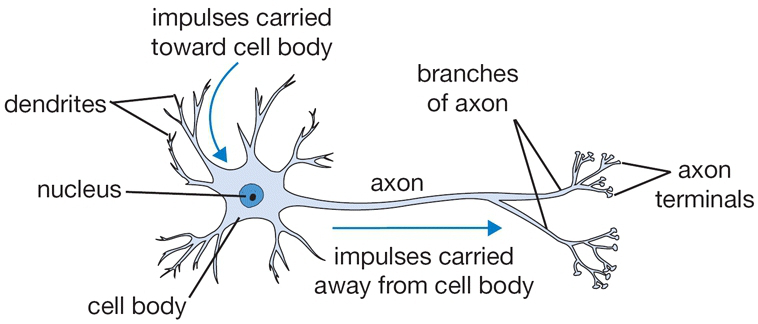
\includegraphics[width=0.6\columnwidth]{images/chap2/neuron.png}
    \footcaption{Cấu tạo một neural thần kinh}
    \label{chap2:animal_neural}
    \end{figure}
\end{center}
\footnotetext{Source: \url{http://cs231n.github.io/neural-networks-1/}}

\begin{center}
    \begin{figure}[H]
    \centering
    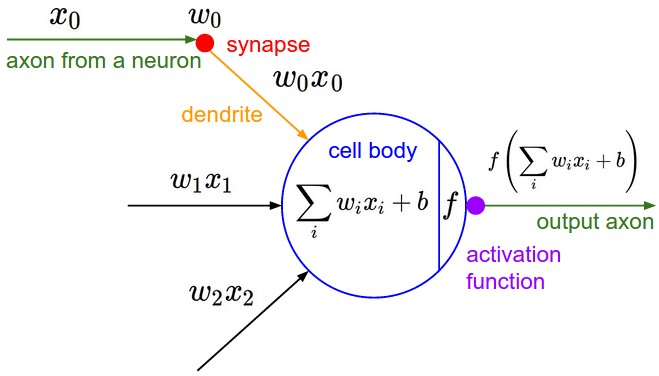
\includegraphics[width=0.6\columnwidth]{images/chap2/neuron_model.jpeg}
    \footcaption{Một mô hình neural dựa trên neural thần kinh}
    \label{chap2:neural_model}
    \end{figure}
\end{center}
\footnotetext{Source: \url{http://cs231n.github.io/neural-networks-1/}}


\subsection{Cấu tạo của neural}
Dựa trên cảm hứng về cấu tạo và hoạt động của mạng nơ-ron sinh học các nhà khoa học đã xây dựng ANN có cấu trúc và cách hoạt động tương tự với mong muốn xây dựng một mô hình mô phỏng lại những khả năng mạnh mẽ của bộ não người và áp dụng vào trong nhiều lĩnh vực khác nhau. Xét về cấu tạo ANN là một mạng lưới nhiều nơ-ron nhân tạo kết nối với nhau, ứng với mỗi cách kết nối ANN sẽ có đặc điểm và khả năng riệng biệt phù hợp với một loại ứng dụng nhất định.

\begin{figure}[H]
  \centering
  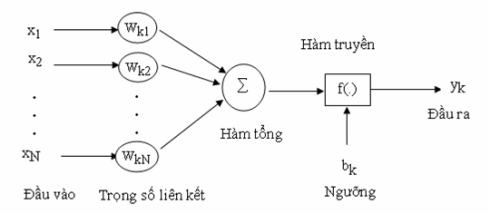
\includegraphics[width=0.9\textwidth]{images/chap2/norolnhantao.png}
  \footcaption{Cấu trúc một neural}
  \label{chap2:neural_structure}    
\end{figure}
\footnotetext{Nguồn: \url{https://tiendv.wordpress.com/2016/11/19/neural-networks/}}
Dựa vào hình \ref{chap2:neural_structure}, ta nhận thấy các thành phần cơ bản của một neural bao gồm:
\begin{description}
    \item[Các giá trị đầu vào] Dữ liệu này thường được đưa vào dưới dạng một vector N chiều
    \item[Các trọng số liên kết] Mỗi giá trị đầu vào được liên kết bởi một trọng số. Trọng số giữa đầu vào thứ j với neural k thường được kí hiện là $\displaystyle w_{kj}$. Các trọng số này lúc đầu sẽ được khởi tạo ngẫu nhiên, sau đó sẽ được cập nhật liên tục trong quá trình học.
    \item[Hàm tổng] Dùng để tính tổng các tích của các giá trị đầu vào với trọng số liên kết của nó.\\
    \begin{center}
        $\displaystyle u_k$ $=$ $\displaystyle \sum_{i=1}^nw_{ki}x_i$
    \end{center}{}
    \item[Ngưỡng] Còn gọi là Bias, là một thành phần của hàm truyền.
    \item[Hàm truyền] Còn gọi là Hàm kích hoạt (activation function), hàm này được dùng để giới hạn đầu ra của neural. Đầu vào của nó là tổng của Hàm tổng và Ngưỡng. Có rất nhiều hàm kích hoạt mà ta sẽ nói đến sau.
     \item[Đầu ra] Là giá trị đầu ra của neural, mỗi neural có nhiều nhất một giá trị đầu ra.
    \begin{center}
       %$\displaystyle y_k = f$$\displaystyle (z_k),$ với\\
       %$\displaystyle z_k = $ $\displaystyle \sum_{i=1}^nw_{ki}x_i + b_k\\
    \end{center}
\end{description}

Một số hàm kích hoạt thông dụng:
\begin{figure}[H]
  \centering
  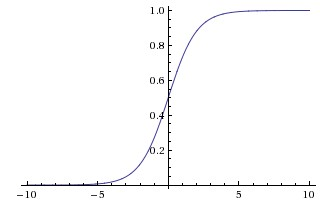
\includegraphics[width=0.5\textwidth]{images/chap2/sigmoid.jpeg}
  \footcaption{Hàm Sigmoid giới hạn đầu ra trong khoảng (0, 1)} 
  \label{chap2:fig08}    
\end{figure}
\footnotetext{Source: \url{http://brohrer.github.io/how_convolutional_neural_networks_work.html}} 

\begin{figure}[H]
  \centering
  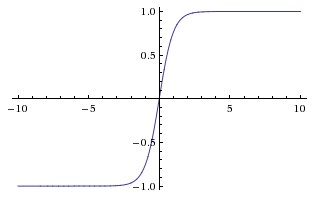
\includegraphics[width=0.5\textwidth]{images/chap2/tanh.jpeg}
  \footcaption{Hàm Tanh giới hạn đầu ra trong khoảng (-1, 1)} 
  \label{chap2:fig08}    
\end{figure}
\footnotetext{Source: \url{http://brohrer.github.io/how_convolutional_neural_networks_work.html}} 

\begin{figure}[H]
  \centering
  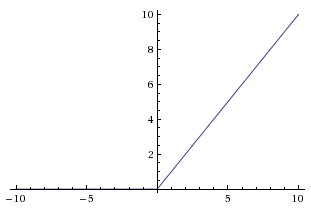
\includegraphics[width=0.5\textwidth]{images/chap2/relu.jpeg}
  \footcaption{Hàm ReLU, bằng 0 khi x < 0 và thuộc đường thẳng có hệ số góc là 1 khi x > 0} 
  \label{chap2:fig08}    
\end{figure}
\footnotetext{Source: \url{http://brohrer.github.io/how_convolutional_neural_networks_work.html}} 

Với các bài toán binary đơn giản, dữ liệu là khả tách tuyến tính, tức là tồn tại một đường thẳng có thể phân chia tập dữ liệu ra làm hai, khả năng biểu diễn của một neural đơn lẻ tỏ ra hiệu quả, tức có thể tìm được một đường thẳng giúp phân chia hai lớp của hàm. Tuy nhiên, trường hợp dữ liệu không khả tách tuyến tính, chúng ta cần kết hợp nhiều neural với nhau tạo thành một mạng neural để có thể giải quyết bài toán phân lớp phi tuyến.


Hình \ref{chap2:neural_logic} mô tả một vài hàm logic đơn giản có thể được biểu diễn dưới một neural và trường hợp phép toán XOR, trường hợp phân lớp phi tuyến, không tìm được lời giải chỉ với một neural.
\begin{center}
    \begin{figure}[H]
    \centering
    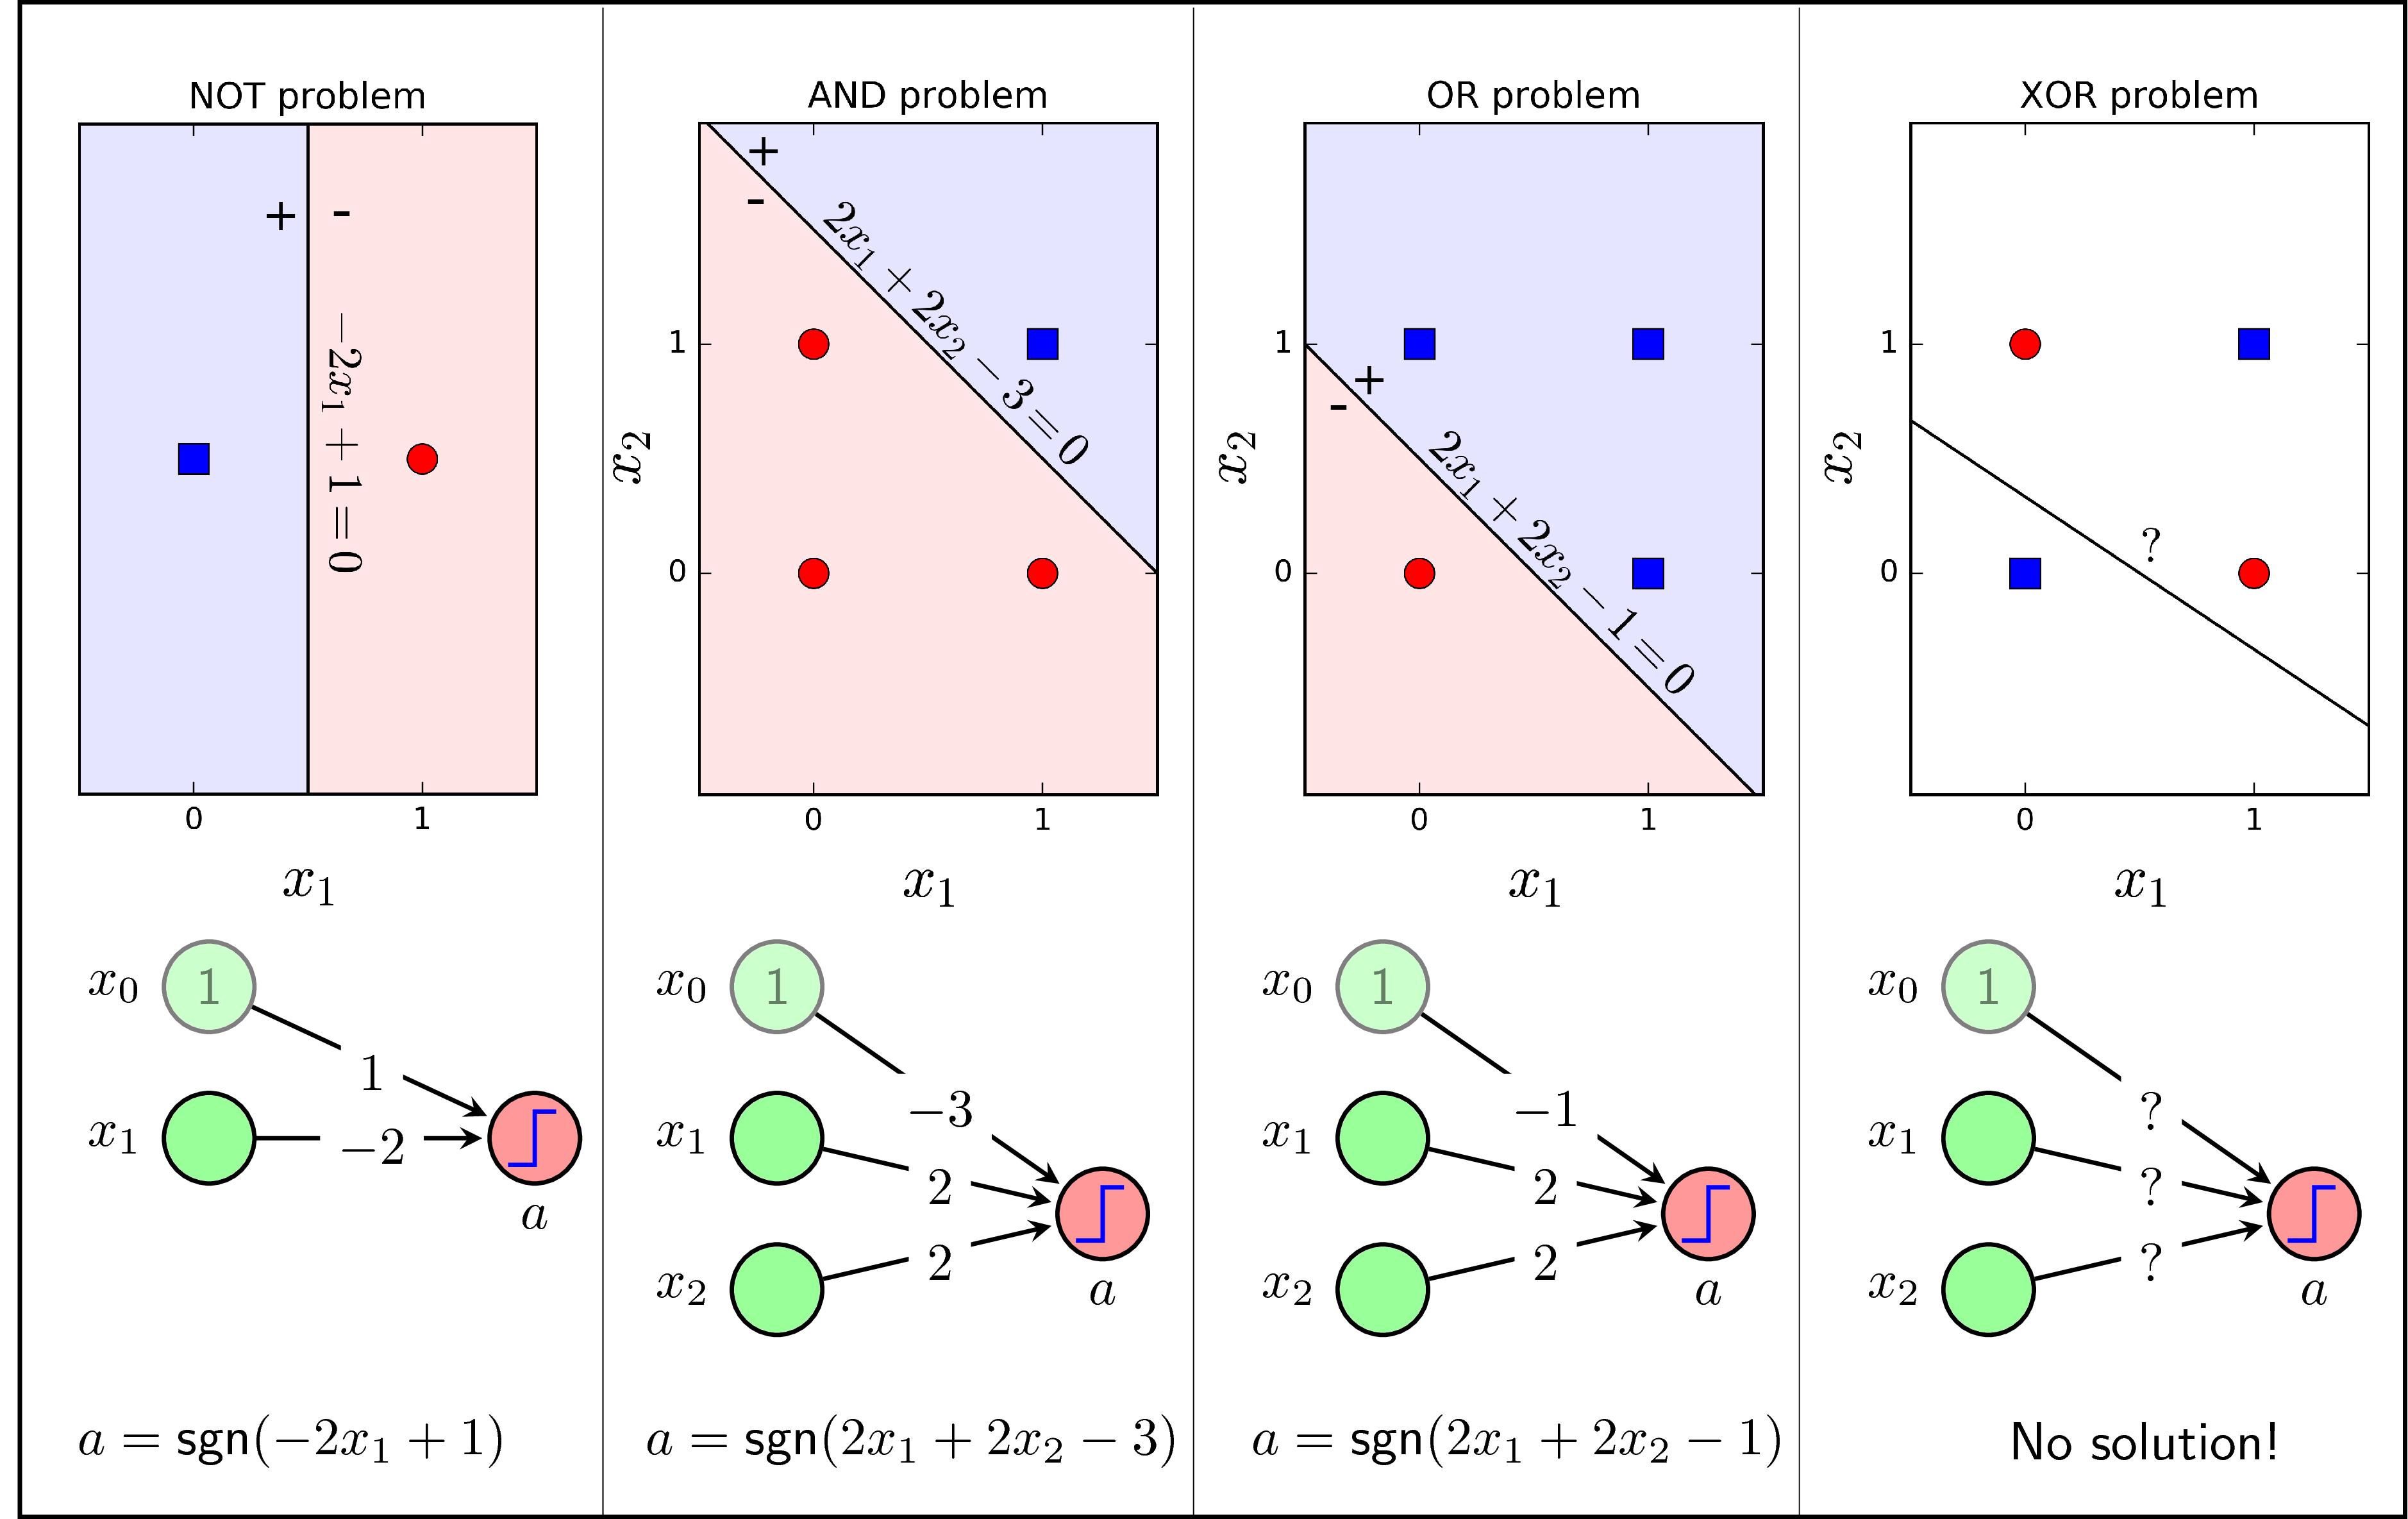
\includegraphics[width=1\columnwidth]{images/chap2/logic_nn.png}
    \footcaption{Mạng neural với một neural có thể biểu diễn được các hàm logic đơn giản}
    \label{chap2:neural_logic}
    \end{figure}
\end{center}
\footnotetext{Source: \url{https://machinelearningcoban.com/2017/02/24/mlp/}}

\subsection{ Cấu trúc mạng neural}
Nhiều neural kết hợp lại tạo thành mạng neural. Tùy vào cách kết nối mà ANN tạo nên kiến trúc riêng của nó. Có thể hiểu rằng các neural kết nối với nhau bằng cách một hoặc một vài đầu ra của neural này có thể là đầu vào của neural khác.

ANN thường được cấu trúc từ các lớp (layer) riêng biệt, các lớp thường là lớp kết nối đầy đủ (fully-connected layer - FC) hoặc lớp kết nối một phần (spartially-connected layer), nhưng phổ biến hơn cả vẫn là các lớp kết nối đầy đủ.

\begin{center}
    \begin{figure}[H]
    \centering
    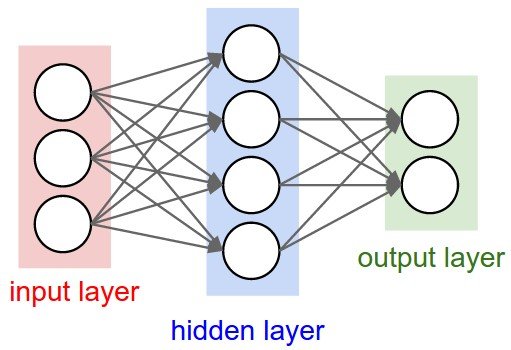
\includegraphics[width=0.5\columnwidth]{images/chap2/2layer.jpeg}
    \footcaption{Mạng neural hai lớp đầy đủ, với một lớp đầu vào 3 neural, lớp ẩn 4 neural và lớp đầu ra 2 neural. Các neural ở lớp khác nhau kết nối với nhau và không kết nối với các neural trong cùng lớp}
    \label{fig:my_label}
    \end{figure}
\end{center}
\footnotetext{Source: \url{http://cs231n.github.io/neural-networks-1/}}
\begin{center}
    \begin{figure}[H]
    \centering
    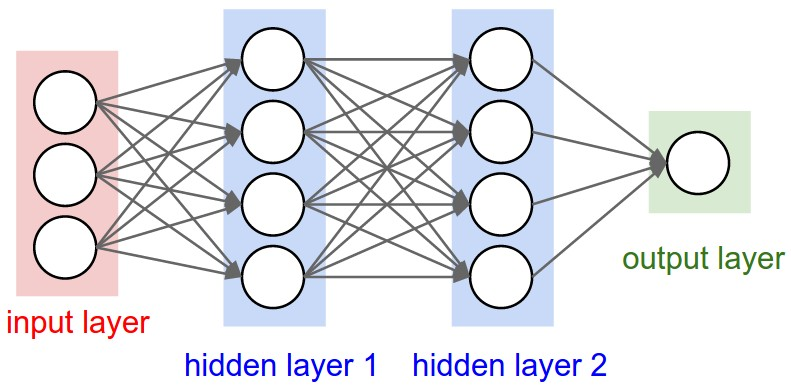
\includegraphics[width=0.6\columnwidth]{images/chap2/3layer.jpeg}
    \footcaption{Mạng neural ba lớp đầy đủ với hai lớp ẩn, mỗi lớp 4 neural}
    \label{fig:my_label}
    \end{figure}
\end{center}
\footnotetext{Source: \url{http://cs231n.github.io/neural-networks-1/}}


\begin{center}
    \begin{figure}[H]
    \centering
    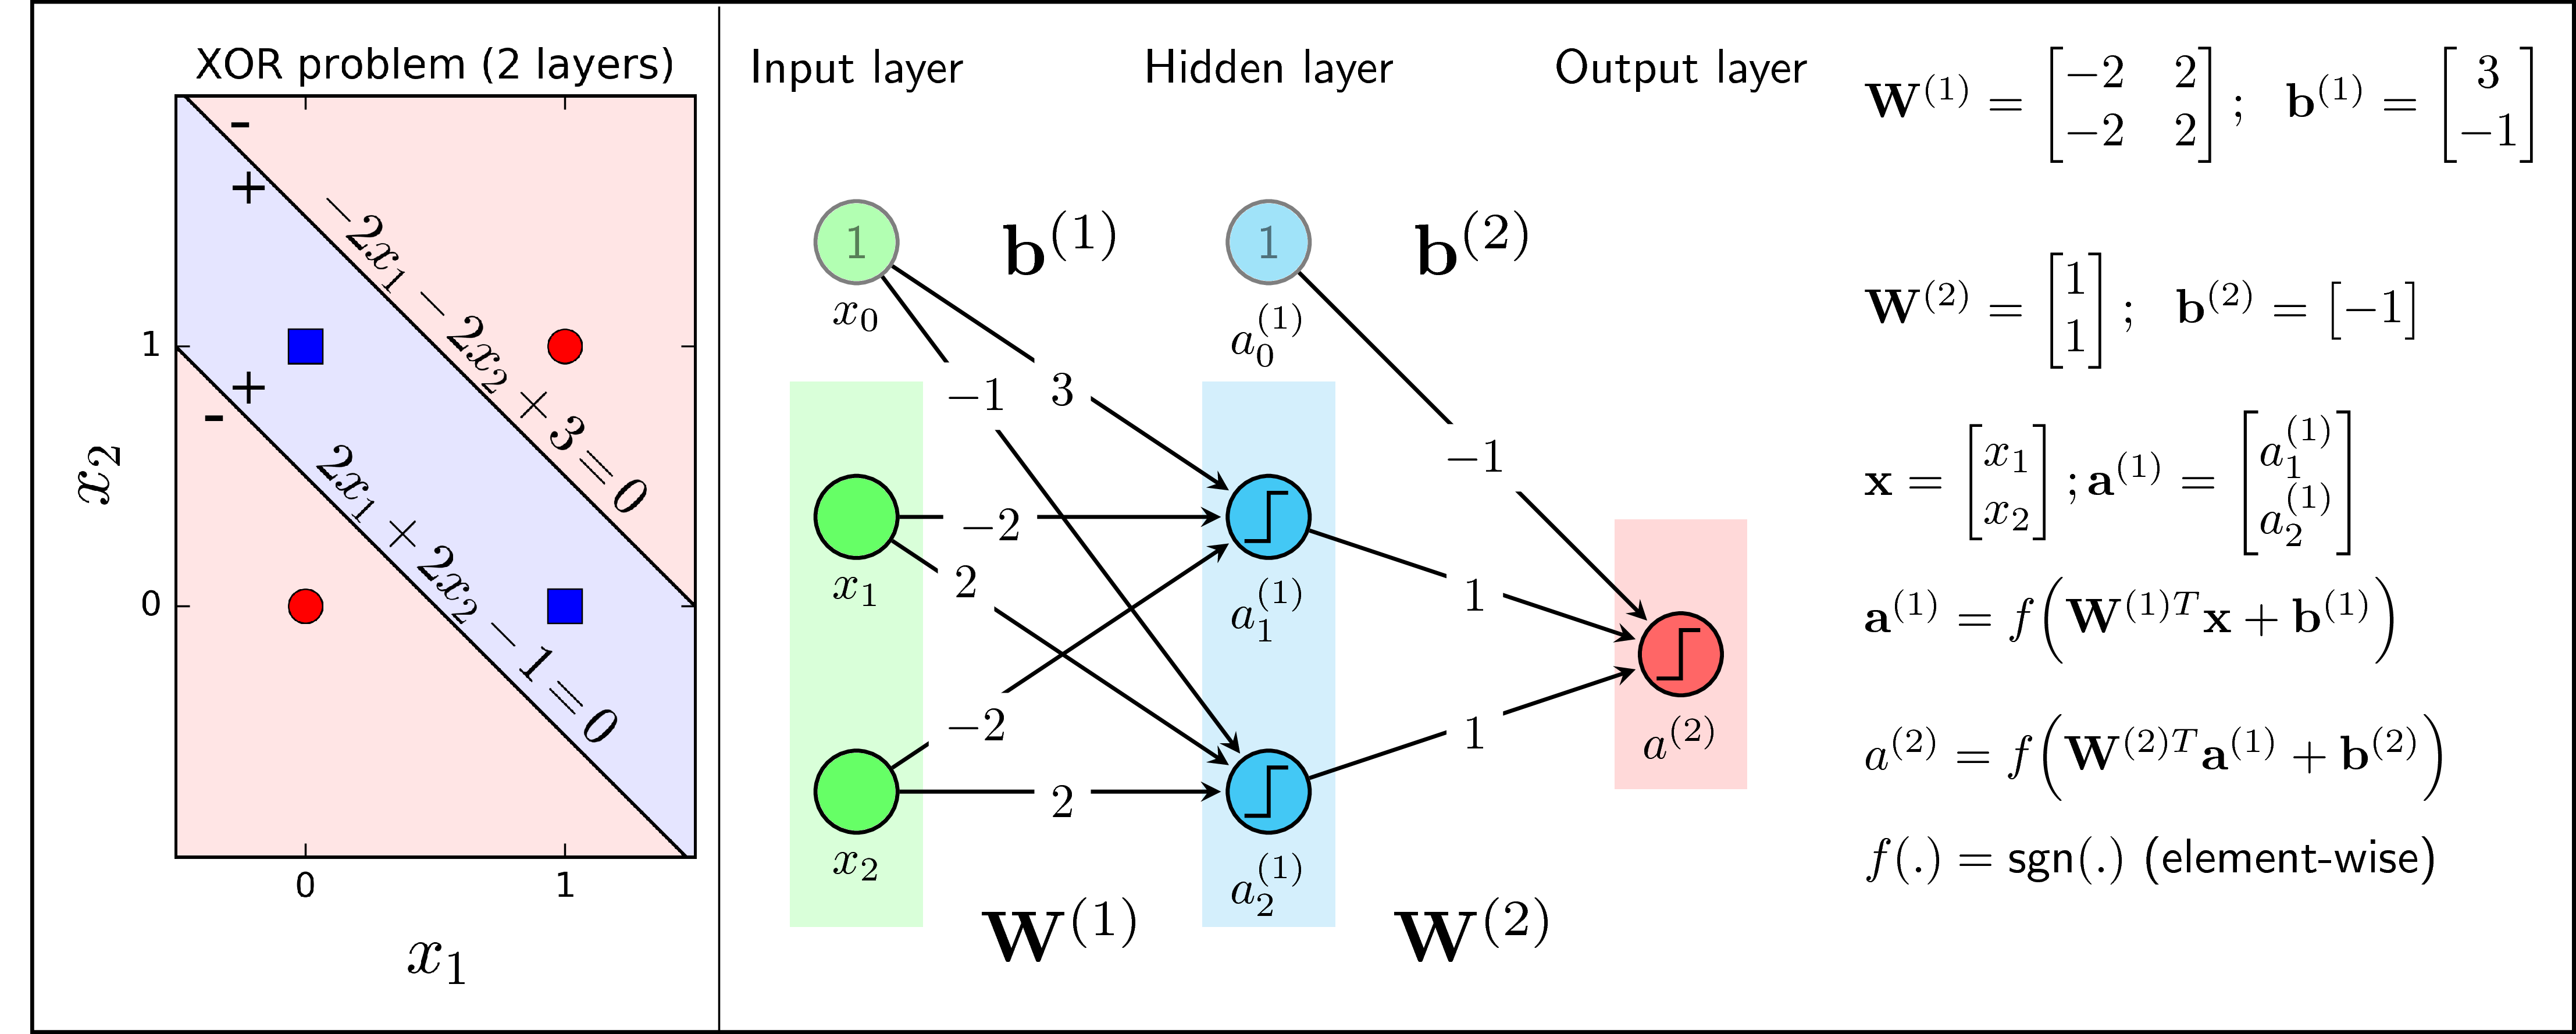
\includegraphics[width=1\columnwidth]{images/chap2/xor_nn.png}
    \footcaption{Mạng neural biểu diễn hàm XOR}
    \label{fig:my_label}
    \end{figure}
\end{center}
\footnotetext{Source: \url{https://machinelearningcoban.com/2017/02/24/mlp/}}
Mạng neural trở nên hiệu quả hơn với các dữ liệu phân bố phi tuyến. Tuy vậy, lựa chọn số lớp ẩn là một vấn đề không hề đơn giản. Về cơ bản, số lớp tăng cũng như kích thước mạng tăng, các neural sẽ biểu diễn được nhiều hàm phức tạp hơn, nhưng từ đó cũng dễ dẫn đến overfit hơn. 

\begin{center}
    \begin{figure}[H]
    \centering
    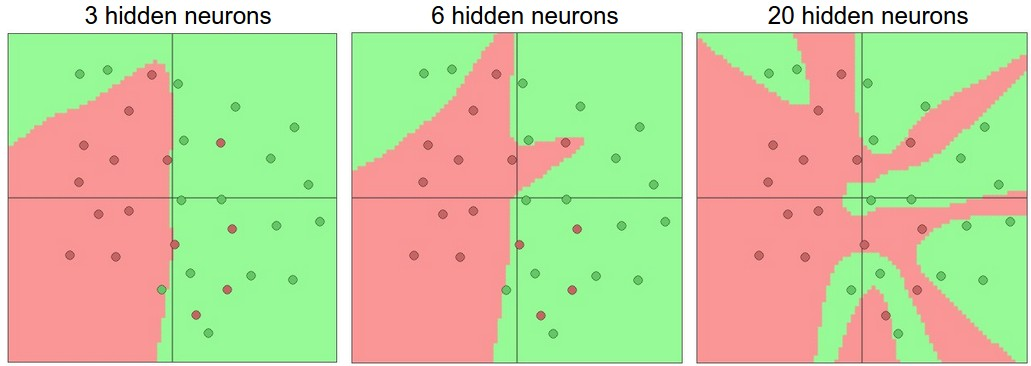
\includegraphics[width=1\columnwidth]{images/chap2/layer_sizes.jpeg}
    \footcaption{Ba mạng neural khác nhau cho cùng một tập dữ liệu, sau khi được huấn luyện cho ra ba kết quả khác nhau}
    \label{chap2:three_net}
    \end{figure}
\end{center}
\footnotetext{Source: \url{http://cs231n.github.io/neural-networks-1/}}

Ta có thể thấy từ hình \ref{chap2:three_net}, mô hình 3 lớp ẩn không hoàn toàn tổng quát hóa được các lớp của dữ liệu. Trong khi đó, mô hình 20 lớp ẩn bị overfit do nó phân lớp cả những điểm nhiễu. Nhưng đừng vì vậy mà chọn mô hình nhỏ hơn chỉ vì nó không bị overfit.

Trong thực tế, người ta không chọn những mô hình nhỏ hơn để tránh overfit, vì những mô hình này không hiệu quả với các thuật toán huấn luyện local như Gradient Descent (GD), thay vào đó, họ vẫn chọn mô hình lớn nhất phần cứng có thể hỗ trợ được, sau đó kết hợp các kĩ thuật xử lí, giảm thiểu nhiễu và overfit để đạt được kết quả khả quan hơn.

\subsection{Hàm mất mát}
Hàm mất mát, kí hiệu là \textbf{L}, là một thành phần của \textbf{\(L_D\)}. Trong công thức:
\begin{center}
	\begin{equation}
		L_D(f_w) = \frac{1}{\lvert D \rvert}\sum_{(x, y)\in D}L(f_w(x), y)
	\end{equation}
\end{center}
\textbf{\(L_D\)} là tổng của trung bình cộng các \textbf{L}. Hàm mất mát trả về một số thực không âm thể hiện sự chênh lệch giữa hai đại lượng \textbf{\^{y}}- label được dự đoán, và \textbf{y} - label đúng. Hàm này có tác dụng để đo sự sai lệch giữa giá trị dự đoán và giá trị được gán nhãn ban đầu, tức giá trị của hàm càng nhỏ thì độ sai sót càng ít, kết quả dự đoán được càng gần với kết quả mong muốn. Trong trường hợp lý tưởng, tức là khi \textbf{\^{y}} \textbf{ = y}, hàm mất mát đạt giá trị cực tiểu bằng 0.

Ta nhận thấy hàm mất mát của một mô hình phải thỏa mãn các tiêu chí sau:
\begin{itemize}
	\item Hàm mất mát phải liên tục, khả vi, vì các phương pháp thông dụng để cực tiểu hóa hàm mất mát thường đòi hỏi phải tính được đạo hàm
	\item Khi model dự đoán sai, ta cần phải phạt model nhiều hơn khi model dự đoán gần đúng, tức là hàm mất mát sẽ lớn hơn khi model dự đoán một kết quả xa hơn kết quả mong đợi.
\end{itemize}

Một số hàm mất mát cơ bản:
\begin{itemize}
	\item Hàm \textbf{Square Loss}
	\begin{center}
		\begin{equation}
			L(\hat{y}, y) = \frac{1}{2}(\hat{y} - y)^2
		\end{equation}
	\end{center}
	Hàm này thường được dùng cho cả mục đích classification và regression, nhưng vẫn được dùng trong regression nhiều hơn.
	\item Hàm \textbf{0-1 Loss}
	Hàm này trả về 1 nếu \textbf{\^{y}}.\textbf{y} < 0, và trả về 0 nếu ngược lại. Hàm này không có đạo hàm ở điểm 0 nên thường được dùng để tính error rate của mô hình chứ không dùng để huấn luyện mô hình.
	\item Hàm \textbf{Perceptron Loss}
	\begin{center}
		\begin{equation}
			L_{perceptron}(\hat{y}, y) = max(0, \hat{y}.y)
		\end{equation}
	\end{center}
	Đối với \textbf{Perceptron Loss}, mô hình dành cho các bài toán Binary Classification, một trong các đặc điểm là khi mô hình đoán đúng thì \textbf{\^{y}} cùng dấu với \textbf{y}, \textbf{\^{y}}.\textbf{y} < 0. Khi đó:
	\begin{center}
		\begin{equation}
			L_{perceptron}(\hat{y}, y) = max(0, <0) = 0
		\end{equation}
	\end{center}
	Từ đó ta thấy, hàm mất mát này không phân biệt giữa các dự đoán đúng, nhưng lại phạt những dự đoán sai.
	\item Hàm \textbf{Hinge Loss}
	\begin{center}
		\begin{equation}
			L_{hinge}(\hat{y}, y) = max(0, 1-\hat{y}.y)
		\end{equation}
	\end{center}
	Dễ dàng thấy \textbf{Hinge Loss} chính là một biến thể của \textbf{Perceptron Loss}, chỉ là thêm 1 đơn vị vào -\textbf{\^{y}}.\textbf{y}, số 1 này được gọi là \textbf{margin}. Hàm này cho kết quả gần tương tự như \textbf{Perceptron Loss}, chỉ trừ các dự đoán mà \textbf{\^{y}}.\textbf{y} nằm trong khoảng [0, 1]. Kết quả rơi vào khoảng này toàn là kết quả đúng, nhưng \textbf{Hinge Loss} muốn phân biệt các kết quả đúng với nhau, nhưng khi \textbf{\^{y}}.\textbf{y} vượt quá 1 thì hàm không phân biệt nữa. Bởi vì khi nằm trong khoảng [0, 1], kết quả đưa ra là những dự đoán gần ranh giới.
	
Ý tưởng của \textbf{Hinge Loss} là muốn khuyến khích mô hình đưa ra những quyết định có tính chắc chắn cao, nằm ngoài ranh giới để không bị phạt nữa.
	\item Hàm \textbf{Logistic Loss}
	\begin{center}
		\begin{equation}
			L(\hat{y}, y) = log_2(1 + exp(-\hat{y}.y))
		\end{equation}
	\end{center}
	Đây là một hàm liên tục, không âm và không tăng. Một điểm khác biệt giữa \textbf{Logistic Loss} với hai hàm mất mát ở trên là đồ thị của nó có một độ cong nhất định, tức là nó không giảm với tốc độ như nhau ở mọi điểm. Trong khi một phần của \textbf{Perceptron Loss} và \textbf{Hinge Loss} là một đường tuyến tính có tốc độ như nhau tại mọi điểm.
	
	Việc chọn hàm mất mát nào phụ thuộc rất lớn vào tính chất bài toán, ứng dụng và đặc biệt là dữ liệu có sẵn. Hình \ref{chap2:loss_function} dưới đây là đồ thị trực quan từng hàm mất mát.
	\begin{center}
    \begin{figure}[H]
    \centering
    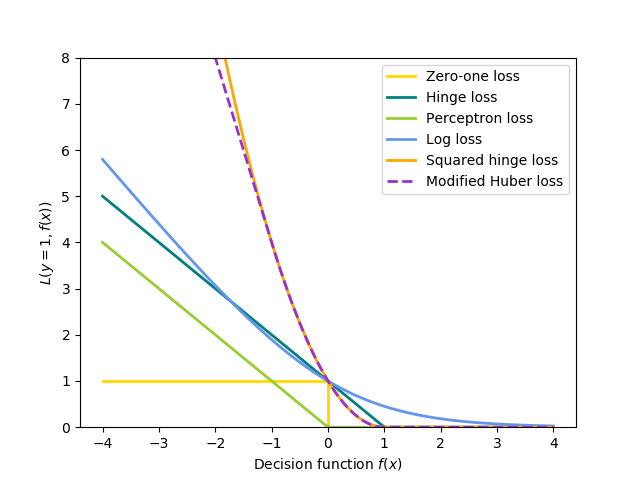
\includegraphics[width=0.7\columnwidth]{images/chap2/loss_plot.png}
    \caption{Đồ thị các hàm mất mát}
    \label{chap2:loss_function}
    \end{figure}
\end{center}
\end{itemize}

\subsection{Giải thuật lan truyền ngược (Backpropagation)}
Có thể hiểu mạng neural nhân tạo là một mạng nhận vào một tập các dữ liệu huấn luyện \textbf{X}, sau quá trình huấn luyện sẽ cho ra một tập weight \textbf{W} và bias \textbf{b}. Hàm \textbf{f(W, b, x)}  với x là input của bài toán, chính là mô hình thu được bằng mạng neural nhân tạo. Mạng càng chính xác thì \textbf{f(W, b, x)} càng cho kết quả gần với thực tế.

Có nhiều phương pháp để tối ưu \textbf{W}, nhưng phổ biến nhất vẫn là sử dụng \textbf{Gradient Descent} (GD). Để áp dụng GD, ta cần tính hàm mất mát của mô hình theo W và b. Giả sử \textbf{J(W, b, x)} là một hàm mất mát, để áp dụng GD, ta phải tính được:
\begin{center}
	\begin{equation}
		\frac{\partial J}{\partial W};
		\frac{\partial J}{\partial b}
	\end{equation}
\end{center}
Ví dụ hàm mất mát là hàm Square Loss, ta có:
\begin{center}
	\begin{equation}
		J(W, b, x) = \frac{1}{N}\sum_{n=1}^N||y_n - \hat{y}_n||^2_2
	\end{equation}
\end{center}
Với N là số mẫu trong tập training.

Theo công thức ở trên, hàm mất mát không phụ thuộc trực tiếp vào W và b, nên việc tính đạo hàm \(\frac{\partial J}{\partial W}\) và \(\frac{\partial J}{\partial b}\) là rất phức tạp. Do vậy, thuật toán Backpropagation thường được sử dụng cùng với gradient để tính ngược từ lớp cuối cùng về lớp đầu tiên nhằm tìm lượng thay đổi \(\Delta W\) hay \(\Delta b\) tương ứng giúp tối ưu hóa W và b.

Lớp cuối cùng được tính đầu tiên vì nó gần với lớp ouput và hàm mất mát nhất. Đạo hàm các lớp trước được tính theo quy tắc \textit{chain rule}, tức đạo hàm của hàm hợp.

Ví dụ, đạo hàm của hàm mất mát của trọng số ở lớp cuối cùng:
\begin{center}
	\begin{equation}
		\frac{\partial J}{\partial w_{ij}^{(L)}} = \frac{\partial J}{\partial z_j^{(L)}}.\frac{\partial z_j^{(L)}}{\partial w_{ij}^{(L)}} 
		= e_j^{(L)}a_i^{(L-1)}
	\end{equation}
\end{center}
Trong đó \(\frac{\partial z_j^{(L)}}{\partial w_{ij}^{(L)}} = a_i^{(L-1)}\) vì \(z_j^{(L)} = w_j^{(L)}a^{(L-1)}+b_j^{(L)}\)
Tương tự, đạo hàm của hàm mất mát theo b ở lớp cuối cùng:
\begin{center}
	\begin{equation}
		\frac{\partial J}{\partial b_{j}^{(L)}} = \frac{\partial J}{\partial z_j^{(L)}}.\frac{\partial z_j^{(L)}}{\partial b_{j}^{(L)}} 
		= e_j^{(L)}
	\end{equation}
\end{center}
Hình \ref{chap2:backpropagation} dưới đây mô tả trực quan cách tính Backpropagation qua các biến số và các lớp của mạng:
\begin{center}
    \begin{figure}[H]
    \centering
    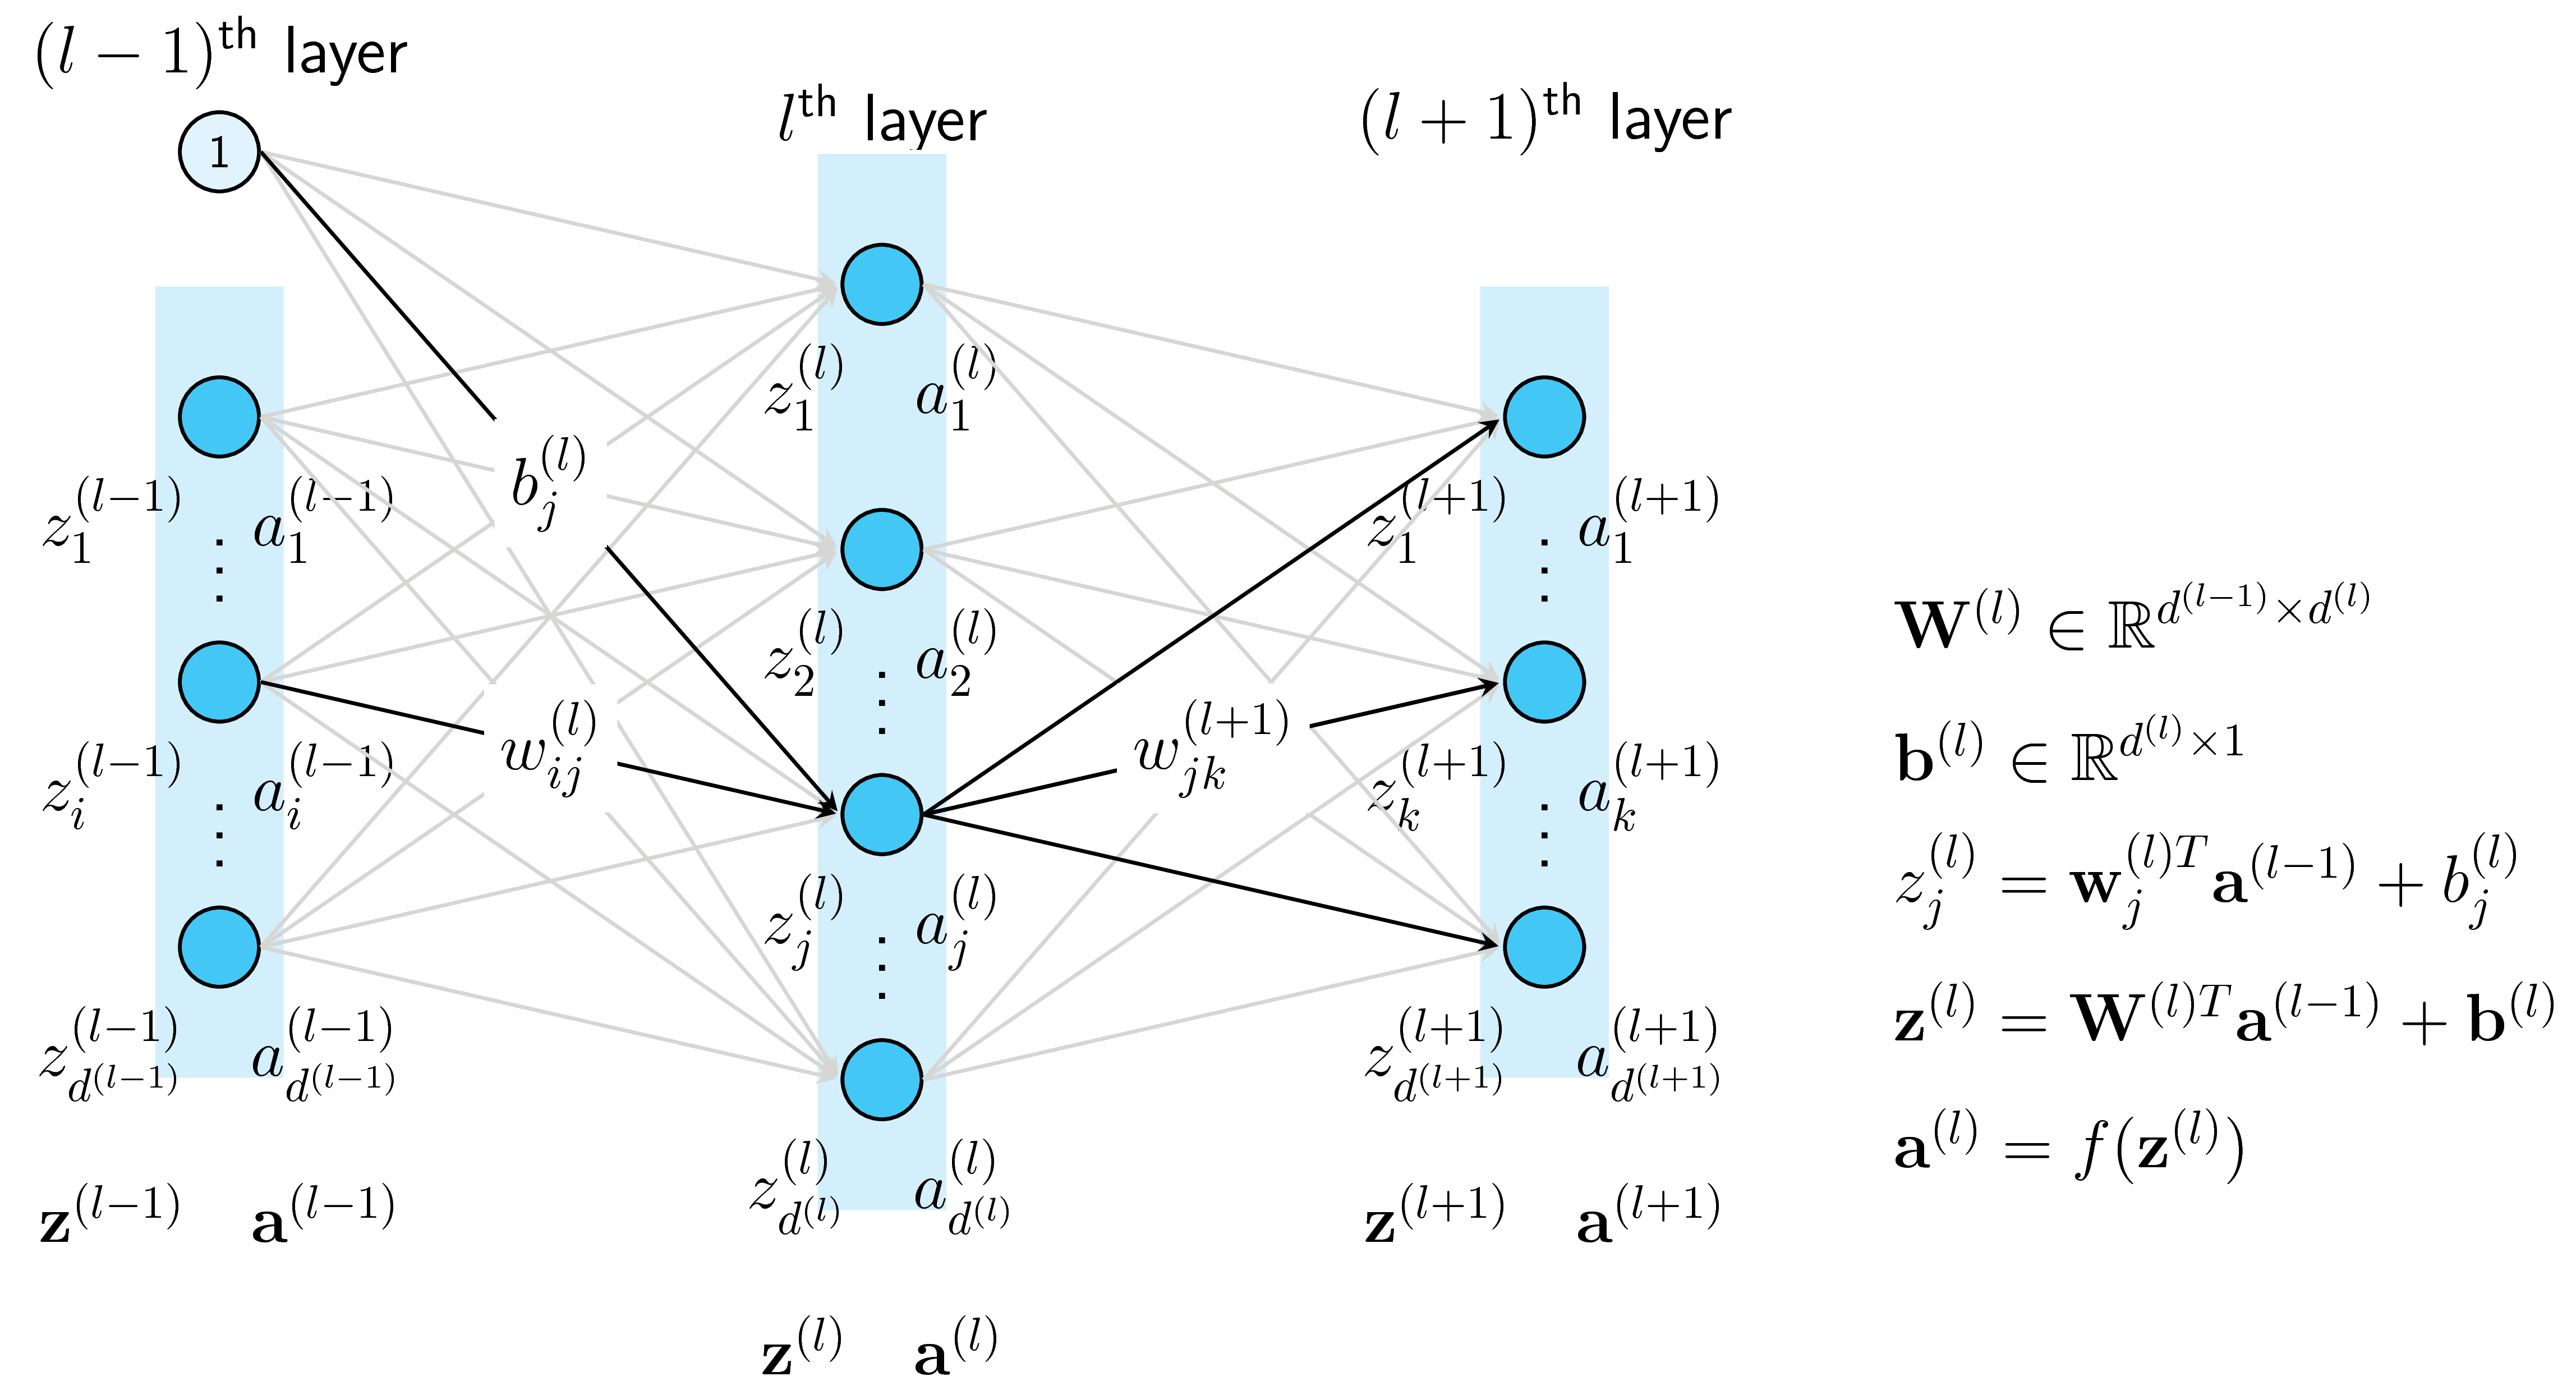
\includegraphics[width=1\columnwidth]{images/chap2/backpropagation.png}
    \footcaption{Cách tính Backpropagation}
    \label{chap2:backpropagation}
    \end{figure}
\end{center}
\footnotetext{Source: \url{https://machinelearningcoban.com/2017/02/24/mlp/}}
Từ hình trên ta có:
\begin{center}
	\begin{equation}
		\frac{\partial J}{\partial w_{ij}^{(l)}} = \frac{\partial J}{\partial z_j^{(l)}}.\frac{\partial z_j^{(l)}}{\partial w_{ij}^{(l)}} 
		= e_j^{(l)}a_i^{(l-1)}
	\end{equation}
\end{center}
trong đó:
\begin{align}
		e_j^{(l)} & = \frac{\partial J}{\partial z_j^{(l)}} = \frac{\partial J}{\partial a_j^{(l)}}.\frac{\partial a_j^{(l)}}{\partial z_j^{(l)}} \nonumber\\
		& = (\sum_{k=1}^{d^{(l+1)}} \frac{\partial J}{\partial z_k^{(l+1)}}.\frac{\partial z_k^{(l+1)}}{\partial a_j^{(l)}} )f'(z_j^{(l)}) \nonumber\\
		& = (\sum_{k=1}^{d^{(l+1)}} e_k^{(l+1)}w_{jk}^{(l+1)} )f'(z_j^{(l)}) \nonumber\\
		& = (e^{(l+1)}w_{j:}^{(l+1)})f'(z_j^{(l)}) \nonumber\\
\end{align}
Tương tự ta có hàm mất mát so với b trên từng lớp của mạng:
	\begin{align}
	\frac{\partial J}{\partial b_j^{(l)}} = e_j^{(l)}
\end{align}
Với \( (e_j^{(l+1)} = [e_1^{(l+1)}, e_2^{(l+1)},...,e_{d^{(l+1)}}^{(l+1)}])^T \)

Từ các công thức trên, ta thấy việc tính \(e_j^{(l)}\) rất quan trọng. Muốn tính \(e_j^{(l)}\) ta phải tính được \(e_j^{(l+1)}\), tức tính ngược giá trị này từ cuối. Đó là nguồn gốc cho tên Backpropagation của giải thuật này.

\section{Mạng neural tích chập}
\subsection{Định nghĩa}
Mạng neural nhân tạo ra đời đã được ứng dụng và thành công trong nhiều bài toán phân loại và nhận dạng. Tuy nhiên, ANN không thực sự hiệu quả đối với những dữ liệu có dạng hình ảnh. Chính sự liên kết quá đầy đủ đã tạo nên những khó khăn cho mô hình vì dữ liệu hình ảnh có kích thước khá lớn. Chính vì lẽ đó Mạng neural tích chập ra đời, với ý tưởng thay vì toàn bộ ảnh kết nối với một node, nay một node chỉ cần kết nối với một phần của ảnh, từ đó dữ liệu hình ảnh thông qua các lớp của mô hình này sẽ được huấn luyện thành các đặc điểm (feature) và tiến hành phân lớp.

CNN là một trong những mô hình Deep Learning hiện nay giúp chúng ta giải quyết các vấn đề về thị giác máy tính như nhận diện, phân loại ảnh với độ chính xác cao. Về cơ bản, CNN là một mạng ANN truyền thẳng và bao gồm các lớp sau: lớp \textbf{Convolutional}, lớp \textbf{ReLU}, lớp \textbf{Pooling} và lớp  \textbf{Fully connected}. Số lượng và thứ tự giữa các lớp này sẽ tạo ra những mô hình khác nhau phù hợp cho từng bài toán khác nhau.


Hình \ref{chap2:cnn_example} mô tả cấu trúc một mạng neural tích chập từ input, qua các lớp Convolution, Pooling, Fully Connected đến output.
\begin{center}
    \begin{figure}[H]
    \centering
    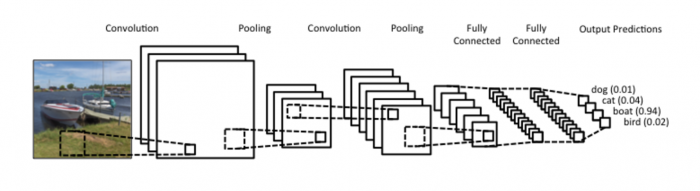
\includegraphics[width=1\columnwidth]{images/chap2/cnn.png}
    \footcaption{Một mạng neural tích chập}
    \label{chap2:cnn_example}
    \end{figure}
\end{center}
\footnotetext{Source: \url{http://www.wildml.com/2015/11/understanding-convolutional-neural-networks-for-nlp/}}

\subsection{Lớp Convolutional}
Lớp Convolutional là lớp quan trọng nhất trong mô hình CNN. Lớp này ra đời dựa trên cơ sở lý thuyết tín hiệu số, việc tính tích chập sẽ giúp trích xuất được những thông tin quan trọng từ hình ảnh. Phép tính này được thực hiện bằng cách trượt một cửa sổ mà ta gọi là sliding window (hoặc kernel, filter hay feature detector) trên ma trận hình ảnh đầu vào, trong đó kết quả phép toán mỗi lần trượt được tính như Hình \ref{chap2:calculation}, với sliding window có kích thước 2x2, trên toàn bộ ma trận kích thước 3x4.

\begin{center}
    \begin{figure}[H]
    \centering
    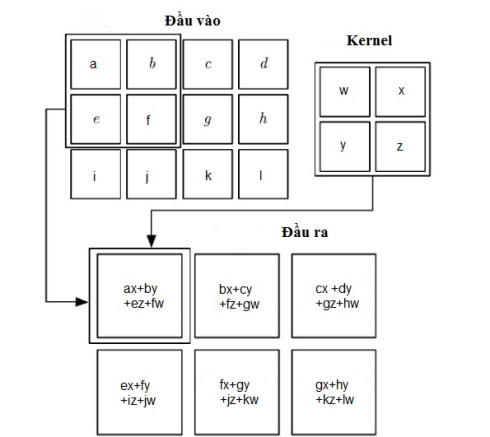
\includegraphics[width=0.6\columnwidth]{images/chap2/viduveconvulution.jpg}
    \caption{Ví dụ về phép tính tích chập}
    \label{chap2:calculation}
    \end{figure}
\end{center}

Số phần tử trong ma trận đầu ra cũng là số ảnh sẽ truyền vào lớp tiếp theo. Trong quá trình huấn luyện, các trọng số của các filder ban đầu sẽ được khởi tạo ngẫu nhiên, sau đó sẽ được cập nhật liên tục.

Sau khi áp dụng các tính toán, ta nhận thấy rằng các thông tin hình ảnh ban đầu đã được biến đổi thành các feature (cạnh, hướng, hình dạng, màu sắc,...). Hình \ref{chap2:result_filter} minh họa việc áp dụng phép tính tích chập lên một ảnh có sẵn.

\begin{center}
    \begin{figure}[H]
    \centering
    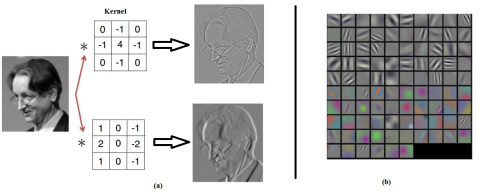
\includegraphics[width=0.8\columnwidth]{images/chap2/viduapplyconvu.jpg}
    \footcaption{(a) Kết quả biến đổi hình ảnh khi thực hiện với các filter khác nhau (b) Các feature được trích xuất từ hình ảnh gốc}
    \label{chap2:result_filter}
    \end{figure}
\end{center}
\footnotetext{Source: \url{http://cs231n.stanford.edu/}}


Đóng vai trò tuy nhỏ nhưng quan trọng trong quá trình này là lớp ReLU (Rectified Linear Unit). Do lớp trước (convolutional) là một phép biến đổi tuyến tính, nên tại mỗi neural cần có một hàm kích hoạt dưới dạng phi tuyến. Có nhiều hàm kích hoạt được sử dụng nhưng các nghiên cứu gần đây cho thấy ReLU có nhiều ưu điểm vượt trội hơn cả, điển hình là cài đặt nhanh và tính toán đơn giản hơn rất nhiều.

Lớp ReLU thường được cài đặt ngay sau lớp Convolutional. Hàm kích hoạt của nó là $f(x) = max(0, x)$, nói một cách trực quan thì lớp này chuyển các giá trị âm từ lớp Convolutional thành 0, nhằm tạo tính phi tuyến cho mô hình (hình \ref{chap2:relu}).
\begin{center}
    \begin{figure}[H]
    \centering
    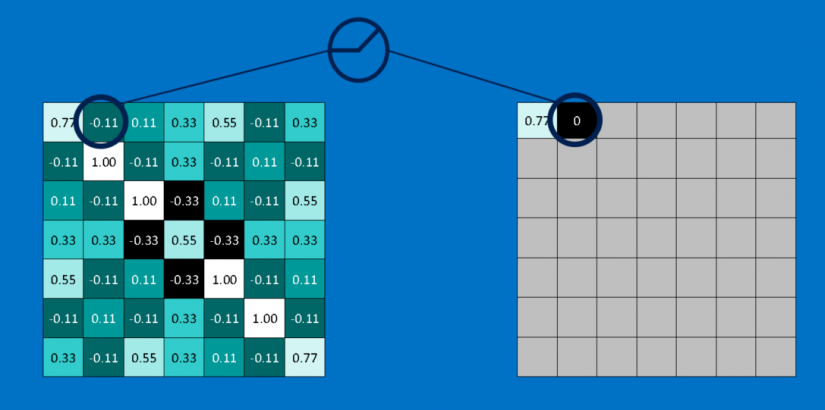
\includegraphics[width=0.8\columnwidth]{images/chap2/relu_array.png}
    \footcaption{Output của layer ReLU giống với output của layer Convolutional, chỉ khác ở chỗ loại bỏ các giá trị âm }
    \label{chap2:relu}
    \end{figure}
\end{center}
\footnotetext{Source: \url{https://brohrer.github.io/how_convolutional_neural_networks_work.html}}

\subsection{Lớp Pooling}
Pooling là một trong những thành phần chính và mạnh mẽ của CNNs. Pooling thực chất là quá trình tính toán trên ma trận để đạt được kết quả là một ma trận nhỏ hơn nhưng vẫn giữ nguyên những feature của ma trận gốc. Pooling tính toán rất đơn giản, với mỗi bước filter trượt trên ảnh gốc, nó sẽ chọn giá trị lớn nhất trong filter đó ở mỗi bước. Như vậy đầu ra sẽ có cùng số lượng hình ảnh nhưng số điểm ảnh lại giảm đáng kể. Ví dụ, giảm số điểm ảnh của một tấm ảnh xuống 4 lần sẽ giúp mọi xử lý trở nên dễ dàng, nhanh chóng.

Một ảnh sau khi qua lớp Pooling vừa được thu nhỏ, vừa bảo toàn tính khớp với mỗi feature. Do đó CNNs vẫn có thể tìm xem liệu một feature có nằm trong hình ảnh hay không, từ đó vẫn cho kết quả chính xác.

\begin{center}
    \begin{figure}[H]
    \centering
    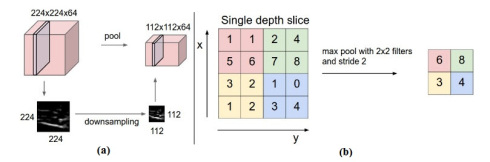
\includegraphics[width=0.8\columnwidth]{images/chap2/pool.jpg}
    \footcaption{Tính toán trên lớp Pooling}
    \label{fig:my_label}
    \end{figure}
\end{center}
\footnotetext{Source: \url{http://cs231n.github.io/convolutional-networks/}}

\begin{center}
    \begin{figure}[H]
    \centering
    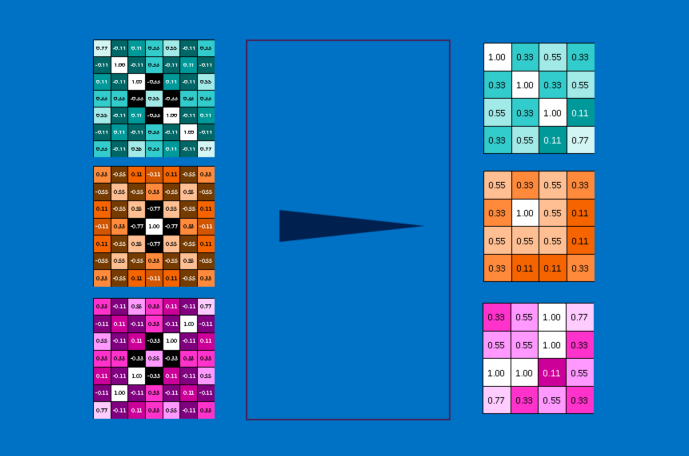
\includegraphics[width=0.6\columnwidth]{images/chap2/resize.png}
    \footcaption{Đầu ra có cùng số lượng ảnh nhưng kích thước bị giảm, tuy vậy vẫn giữ nguyên các feature trước đó}
    \label{fig:my_label}
    \end{figure}
\end{center}
\footnotetext{Source: \url{https://brohrer.github.io/how_convolutional_neural_networks_work.html}}

\subsection{Lớp Fully-connected}
Fully-connected tương tự với lớp trong ANN. Các giá trị ở lớp trước được liên kết đầy đủ vào các node của lớp tiếp theo. Trong CNN, lớp này thường xuất hiện ở các tầng cuối của mô hình. Vì ảnh đã được xử lý và trích xuất feature từ các lớp trước nên dữ liệu sẽ không còn quá lớn, ta dễ dàng sử dụng FC để tiến hành nhận dạng thông qua các vote.

\begin{center}
    \begin{figure}[H]
    \centering
    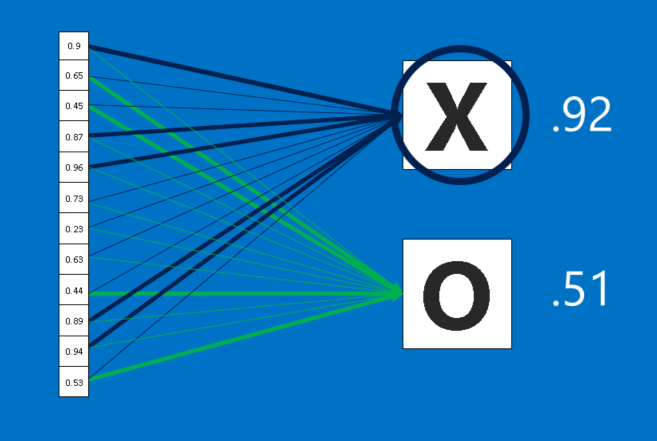
\includegraphics[width=0.5\columnwidth]{images/chap2/fc_vote.png}
    \footcaption{Lớp FC lấy hình ảnh ở các lớp trước rồi chuyển thành các vote (trong hình là phân loại X và O)}
    \label{fig:my_label}
    \end{figure}
\end{center}
\footnotetext{Source: \url{https://brohrer.github.io/how_convolutional_neural_networks_work.html}}

\section{Thuật toán nhận diện hình ảnh}
Có rất nhiều phương pháp nhận diện hình ảnh (Hình \ref{chap2:object_detection_example}), trong đó Faster R-CNN là một trong những phương pháp hiện đại và hiệu quả cho tới ngày nay. Đó là phương pháp phân loại vật thể và xác định vị trí của vật thể đó trong ảnh, trong đó cho output là tọa độ của một hình chữ nhật, đồng thời xác định vật thể bên trong hình chữ nhật đó là gì. Faster R-CNN đã trải qua nhiều phiên bản, trong đó không thể không nhắc tới R-CNN và Fast R-CNN.

\begin{center}
    \begin{figure}[H]
    \centering
    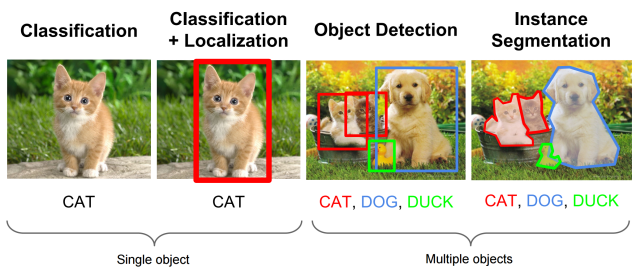
\includegraphics[width=0.6\columnwidth]{images/chap2/LocalizationDetection.png}
    \footcaption{Mô tả bài toán tìm kiếm vị trí vật thể trong ảnh}
    \label{chap2:object_detection_example}
    \end{figure}
\end{center}
\footnotetext{Nguồn: \url{http://cs231n.stanford.edu/slides/2016/winter1516_lecture8.pdf}}
\subsection{Localization bằng phương pháp hồi quy}
Hồi quy có thể được dùng làm phương pháp để xác định được tọa độ của bounding box trong bài toán học có giám sát. Bounding box là khung hình chữ nhật để xác định tọa độ của vật thể trong hình. Trong quá trình huấn luyện mạng nơ-ron, tọa độ này thường được dự đoán ra dưới dạng gồm 4 số ($x_0$, $y_0$, chiều dài, chiều rộng). Kết quả này sẽ được so sánh với tọa độ bounding box của vật đã được gán nhãn. Hàm lỗi khoảng cách Euclidean sẽ được áp dụng để tính lỗi và cập nhật lại trọng số cho mô hình mạng huấn luyện (Hình \ref{fig:2.22}).
\begin{center}
    \begin{figure}[H]
    \centering
    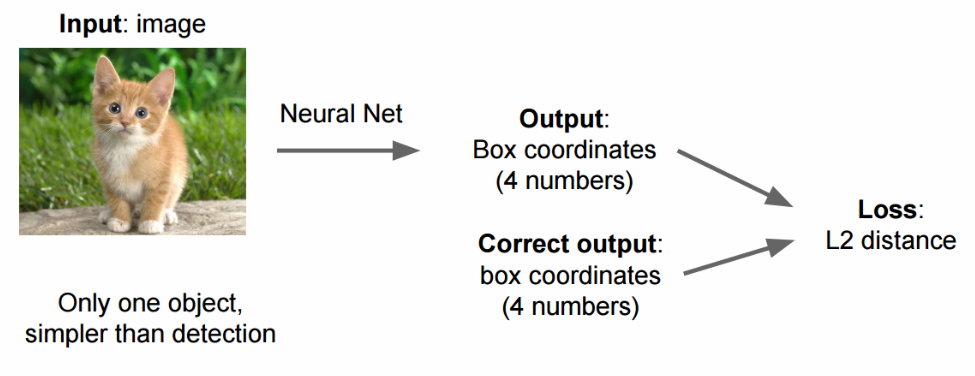
\includegraphics[width=0.8\columnwidth]{images/chap2/localization_1.png}
    \footcaption{Localization bằng phương pháp hồi quy cho mạng nơ-ron}
    \label{fig:2.22}
    \end{figure}
\end{center}
\footnotetext{Nguồn: \url{http://cs231n.stanford.edu/slides/2016/winter1516_lecture8.pdf}}
Cách đơn giản để thực hiện phân loại và localization, gồm có 4 bước:\\
\begin{enumerate}
	\item Huấn luyện một mô hình phân loại hoặc sử dụng mô hình phân loại đã có sẵn (AlexNet, VGG, GoogLeNet)
	\begin{center}
    \begin{figure}[H]
    \centering
    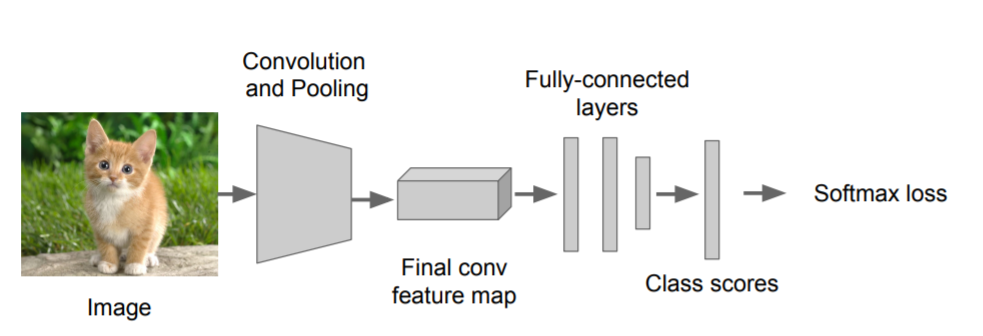
\includegraphics[width=0.8\columnwidth]{images/chap2/localization_2.png}
    \footcaption{Localization bằng phương pháp hồi quy cho mạng nơ-ron - bước 1}
    \label{fig:2.23}
    \end{figure}
	\end{center}
	\footnotetext{Nguồn: \url{http://cs231n.stanford.edu/slides/2016/winter1516_lecture8.pdf}}
	Những mô hình này thường dùng các lớp mạng tích chập và lớp pooling để trích xuất ra feature map (bản đồ đặc trưng), từ đó đưa qua một hoặc nhiều lớp fully-connected để tính được điểm phân loại (Hình \ref{fig:2.23}).
	\item  Thêm các đầu hồi quy vào sau các lớp fully-connected để xác định bounding box
	\begin{center}
    \begin{figure}[H]
    \centering
    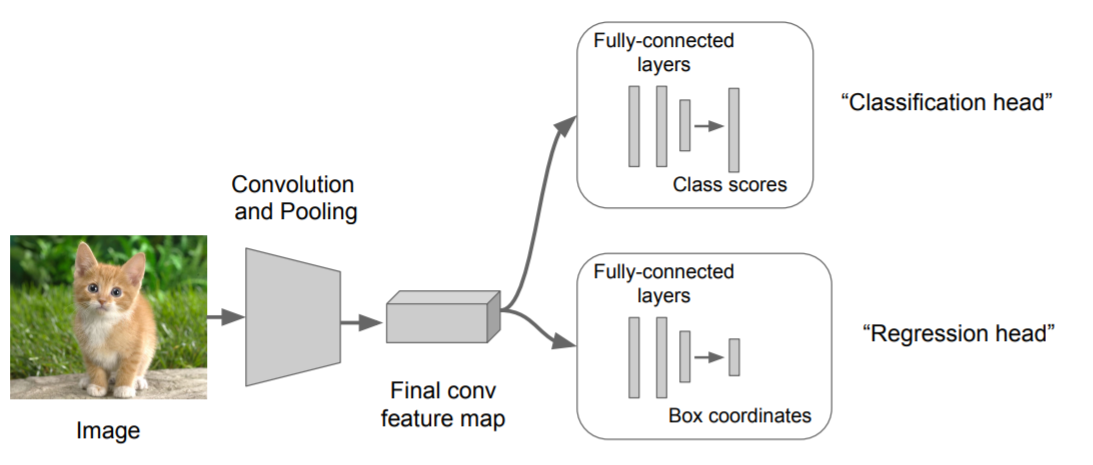
\includegraphics[width=0.8\columnwidth]{images/chap2/localization_3.png}
    \footcaption{Localization bằng phương pháp hồi quy cho mạng nơ-ron - bước 2}
    \label{fig:2.24}
    \end{figure}
	\end{center}
	\footnotetext{Nguồn: \url{http://cs231n.stanford.edu/slides/2016/winter1516_lecture8.pdf}}
	Ở bước này, mô hình mạng được mở thêm một nhánh từ feature map. Nhánh này cũng đi qua một hoặc nhiều lớp fully-connected nhưng nó không dùng để tính điểm phân loại nữa mà sẽ áp dụng phương pháp hồi quy để tính ra tọa độ của bounding box (Hình \ref{fig:2.24}).
	\item Huấn luyện riêng đầu hồi quy với stochastic gradient descent và hàm lỗi L2 (Eclidean distance loss)
	\begin{center}
    \begin{figure}[H]
    \centering
    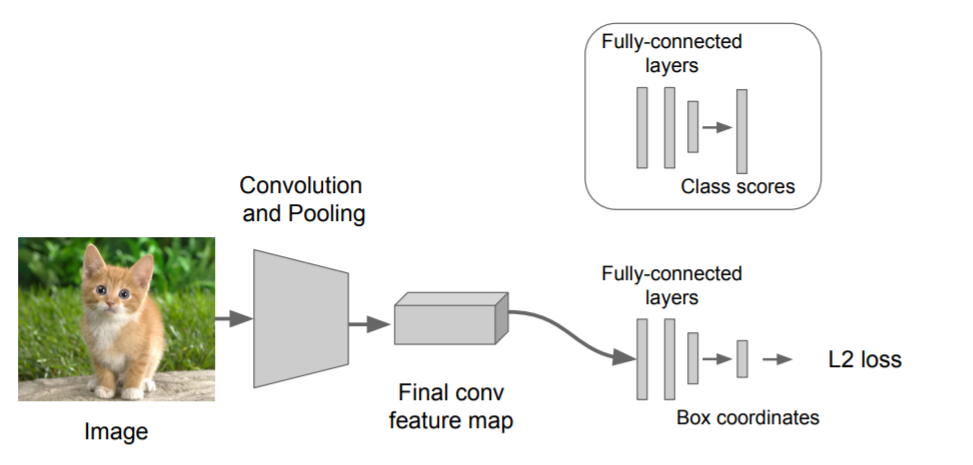
\includegraphics[width=0.8\columnwidth]{images/chap2/localization_4.png}
    \footcaption{Localization bằng phương pháp hồi quy cho mạng nơ-ron - bước 3}
    \label{fig:2.25}
    \end{figure}
	\end{center}
	\footnotetext{Nguồn: \url{http://cs231n.stanford.edu/slides/2016/winter1516_lecture8.pdf}}
	Kết quả dự đoán bounding box sẽ được so với ground-truth box (tọa độ vật thể được gán nhãn trước đó) từ đó tính hàm lỗi và cập nhật lại trọng số cho riêng nhánh mạng hồi quy bằng kĩ thuật stochastic gradient descent (Hình \ref{fig:2.25}).
	\item Dùng cả hai bộ phân loại và hồi quy lúc chạy kết quả
	\begin{center}
    \begin{figure}[H]
    \centering
    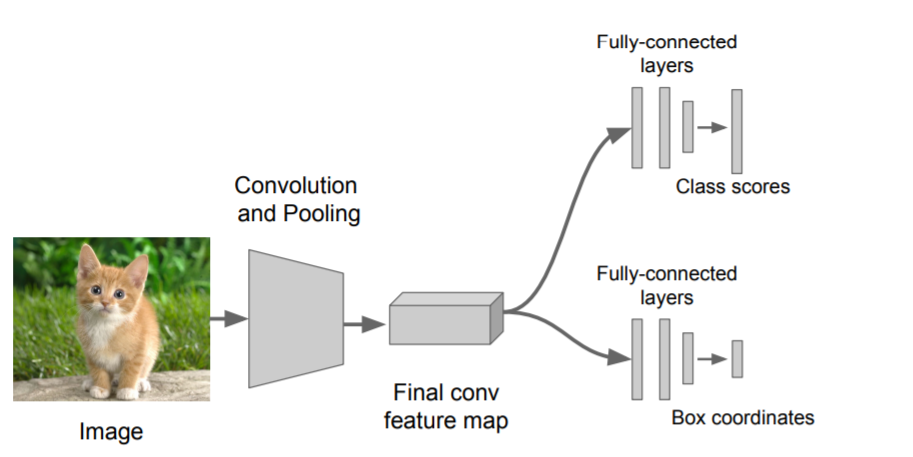
\includegraphics[width=0.8\columnwidth]{images/chap2/localization_5.png}
    \footcaption{Localization bằng phương pháp hồi quy cho mạng nơ-ron - bước 4}
    \label{fig:2.26}
    \end{figure}
	\end{center}
	\footnotetext{Nguồn: \url{http://cs231n.stanford.edu/slides/2016/winter1516_lecture8.pdf}}
	Hàm lỗi L2 được áp dụng để tính lỗi và cập nhật lại trọng số cho nhánh hồi quy dựa theo phương pháp stochastic gradient descent (Hình \ref{fig:2.26}).
\end{enumerate}
Sau khi huấn luyện xong, mô hình có thể sử dụng bằng cách đưa ảnh cần dự đoán vào và thực hiện phân loại cùng với hồi quy để xác định được vật thể thuộc nhãn nào và đánh dấu nó trên hình.
Tuy nhiên hạn chế của phương pháp này chính là chỉ có thể tìm được một vật thể ở mỗi lần hoạt động.
\subsection{Region based Convolutional Neural Network - R-CNN}
R-CNN (Regions + CNN) là một phương pháp nhận diện hình ảnh dựa vào một hệ thống sinh các bounding boxes (hay còn gọi là region proposals), chứa các vùng có khả năng bao gồm các vật thể ở trong.

\begin{center}
    \begin{figure}[H]
    \centering
    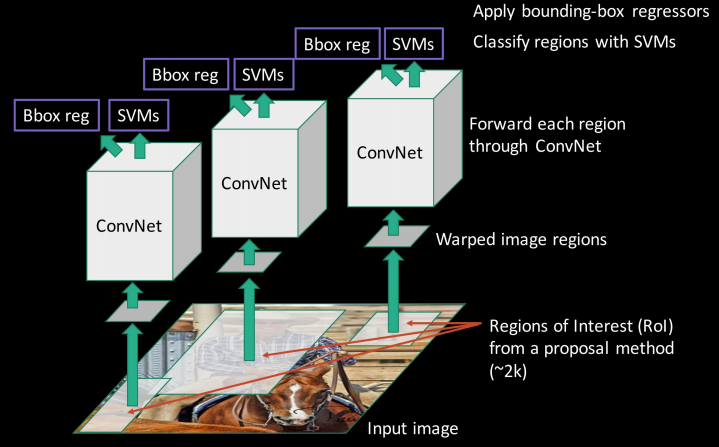
\includegraphics[width=0.6\columnwidth]{images/chap2/RCNNSimple.png}
    \footcaption{Mô hình R-CNN đơn giản}
    \label{fig:2.27}
    \end{figure}
\end{center}
\footnotetext{Nguồn: \url{http://cs231n.stanford.edu/slides/2016/winter1516_lecture8.pdf}}
Hình \ref{fig:2.27} mô tả kiến trúc của mô hình R-CNN, từ ảnh đầu vào ta sẽ tìm các RoI và đưa mỗi RoI qua CNN để trích xuất đặc trưng, cuối cùng dùng SVM và phương pháp hồi quy để phân loại và tìm ra bounding box của vật.
Khuyết điểm lớn nhất của R-CNN chính là thời gian hiện thực. Cụ thể, mô hình được huấn luyện theo các bước như sau:

\begin{enumerate}
    \item Dùng một mạng CNN đã được huấn luyện sẵn (như Alexnet hay VGG-16)
    \begin{center}
    	\begin{figure}[H]
	    \centering
	    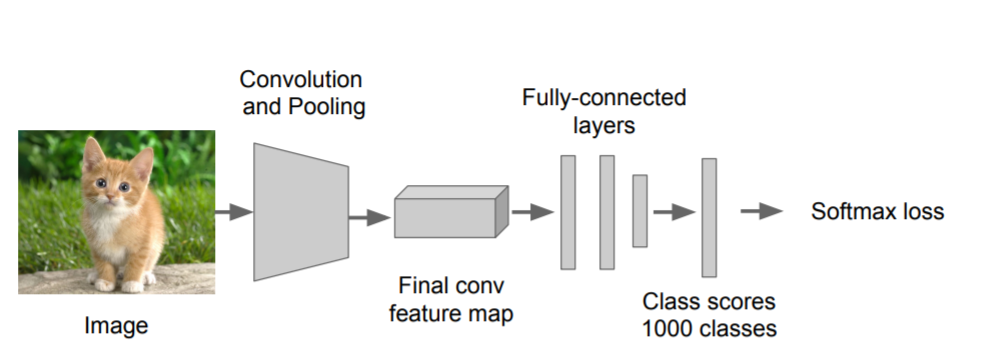
\includegraphics[width=0.8\columnwidth]{images/chap2/rcnn_1.png}
	    \footcaption{Sử dụng một mô hình mạng VGG-16 có sẵn là bộ phân loại 1000 class}
	    \label{fig:2.28}
	    \end{figure}
	\end{center}
	\footnotetext{Nguồn: \url{http://cs231n.stanford.edu/slides/2016/winter1516_lecture8.pdf}}
    \item Sau đó huấn luyện lại layer FC cuối cùng để tính các regions và features của vật thể cần phân loại
    \begin{center}
    	\begin{figure}[H]
	    \centering
	    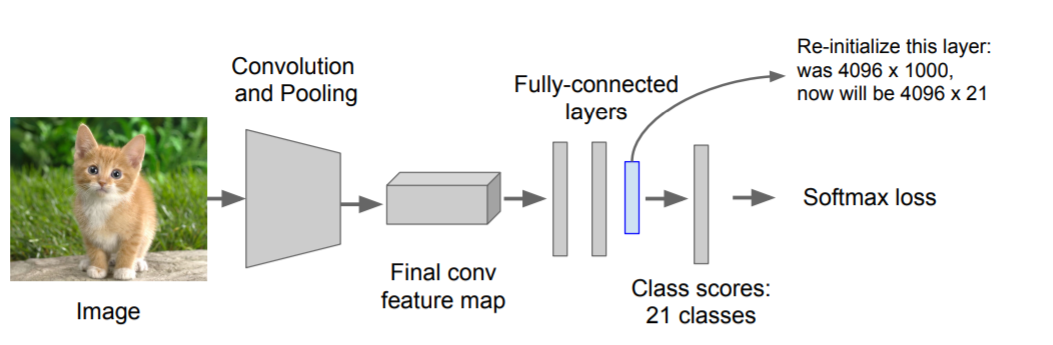
\includegraphics[width=0.8\columnwidth]{images/chap2/rcnn_2.png}
	    \footcaption{Thay lớp fully-connected cuối cùng bằng lớp fully-connected mới với số lượng class mới}
	    \label{fig:2.29}
	    \end{figure}
	\end{center}
	\footnotetext{Nguồn: \url{http://cs231n.stanford.edu/slides/2016/winter1516_lecture8.pdf}}
	Ở hình \ref{fig:2.29}, thay vì dùng 1000 loại, nếu chúng ta chỉ cần phân loại 20 loại thì ta điều chỉnh lớp fully-connected cuối cùng từ $4096 \times 1000$ thành $4096 \times 21$ (20 loại + 1 loại là background, hình ví dụ bên trên), với 4096 là chiều dài của một vector trong lớp fully-connected. Ta bỏ đi lớp fully-connected cuối cùng, lớp được dùng để đưa ra kết quả phân loại 1000 loại, và thay bằng lớp fully-connected cho ra kết quả phân loại là 21 loại. Tiến hành huấn luyện cho mô hình mạng này để đạt được bộ trọng số thích hợp.
    \item Bước này là bước trích xuất đặc trưng của ảnh, ở đây nó lấy tất cả proposal được trích xuất ra từ trong ảnh (xấp xỉ 2000 proposals một ảnh), thay đổi kích cỡ cho phù hợp với đầu vào của CNN rồi dùng CNN chạy feed forward để lấy được các đặc trưng của ảnh sau đó lưu lại.
    \begin{center}
    	\begin{figure}[H]
	    \centering
	    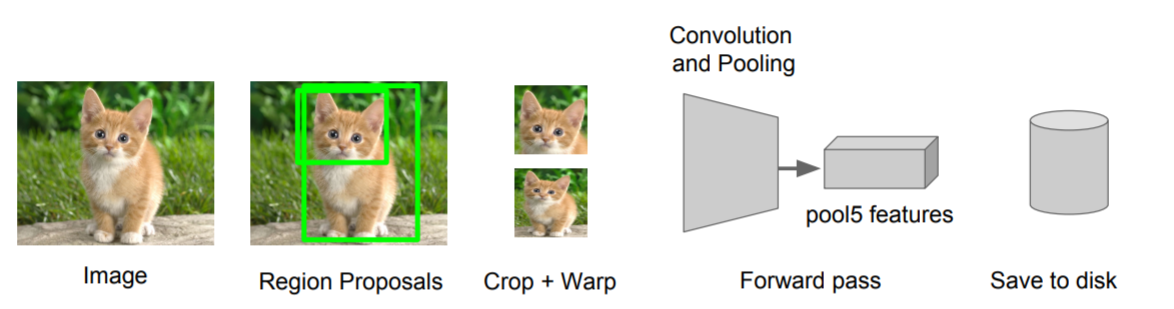
\includegraphics[width=0.8\columnwidth]{images/chap2/rcnn_3.png}
	    \footcaption{Trích xuất đặc trưng của các region proposal}
	    \label{fig:2.30}
	    \end{figure}
	\end{center}
	\footnotetext{Nguồn: \url{http://cs231n.stanford.edu/slides/2016/winter1516_lecture8.pdf}}
	Các region proposal được tìm thấy nhờ sử dụng thuật toán selective search \cite{uijlings2013selective}.
	
	Mỗi proposal được đưa vào mô hình mạng để trích xuất ra được đặc trưng ở cuối các lớp convolutional (Hình \ref{fig:2.30}). Lưu ý rằng bộ dữ liệu nè sẽ có kích thước rất lớn nên cần được lưu trữ vào một vùng nhớ có kích thước lớn.
    \item Huấn luyện SVM phân loại các đặc trưng là thuộc loại nào (với mỗi lớp dùng một SVM nhị phân)
    \begin{center}
    	\begin{figure}[H]
	    \centering
	    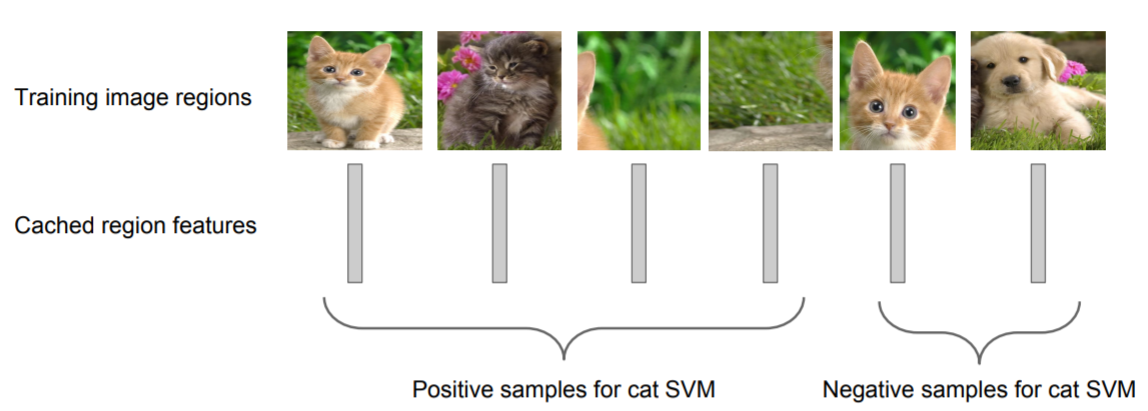
\includegraphics[width=0.8\columnwidth]{images/chap2/rcnn_4_1.png}
	    \footcaption{SVM phân loại cho cat và không phải cat}
	    \label{fig:2.31}
	    \end{figure}
	\end{center}
	\footnotetext{Nguồn: \url{http://cs231n.stanford.edu/slides/2016/winter1516_lecture8.pdf}}
    \begin{center}
    	\begin{figure}[H]
	    \centering
	    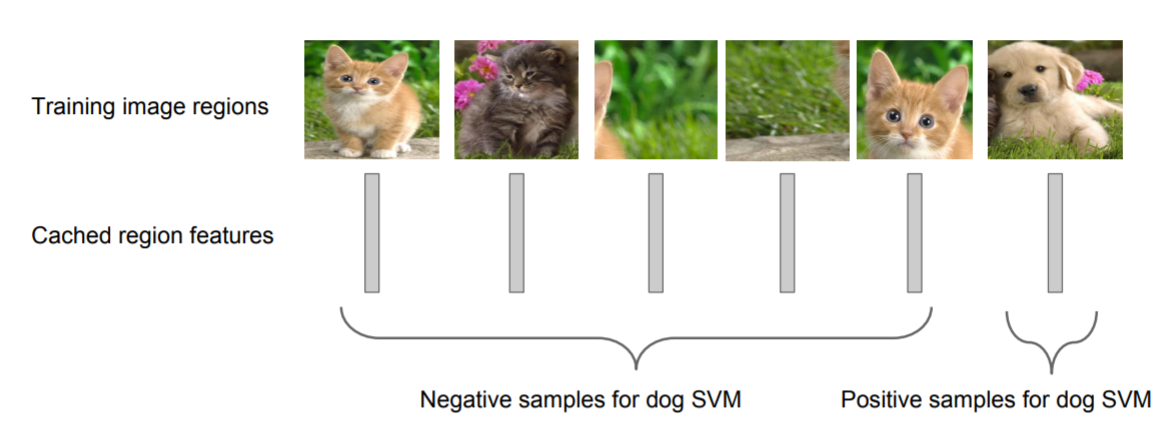
\includegraphics[width=0.8\columnwidth]{images/chap2/rcnn_4.png}
	    \footcaption{SVM phân loại cho dog và không phải dog}
	    \label{fig:2.32}
	    \end{figure}
	\end{center}
	\footnotetext{Nguồn: \url{http://cs231n.stanford.edu/slides/2016/winter1516_lecture8.pdf}}
	Hình \ref{fig:2.31} và \ref{fig:2.32} thể hiện cho hai loại SVM được dùng, một loại để phân biệt có phải cat hay không, một loại dùng để phân biệt có phải dog hay không.
    \item Huấn luyện Linear Regression model để hiệu chỉnh tọa độ các đỉnh của bounding boxes
    \begin{center}
    	\begin{figure}[H]
	    \centering
	    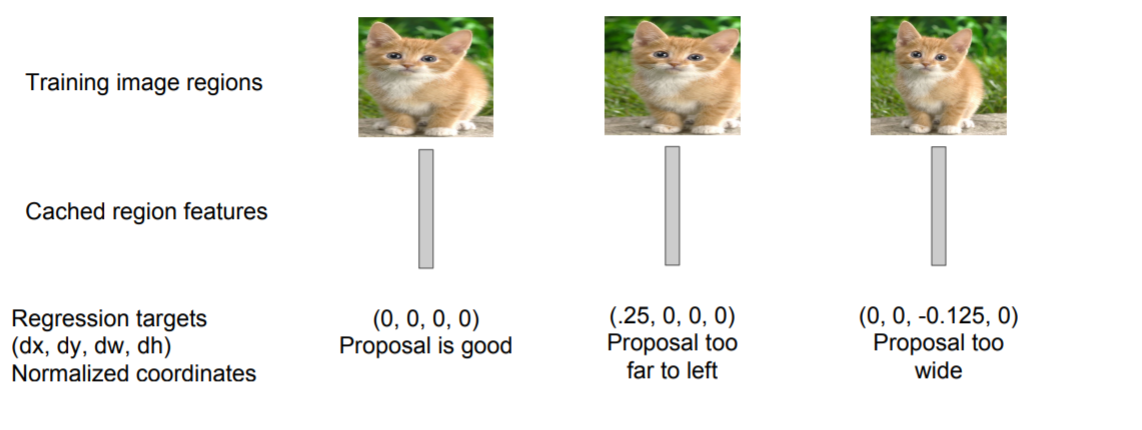
\includegraphics[width=0.8\columnwidth]{images/chap2/rcnn_5.png}
	    \footcaption{Thay lớp fully-connected cuối cùng bằng lớp fully-connected mới}
	    \label{fig:2.33}
	    \end{figure}
	\end{center}
	\footnotetext{Nguồn: \url{http://cs231n.stanford.edu/slides/2016/winter1516_lecture8.pdf}}
	Tọa độ của bounding box dự đoán ra sẽ được so sánh với dữ liệu được gán nhãn, từ đó tính lỗi và cập nhật lại trọng số (Hình \ref{fig:2.33}).
\end{enumerate}
R-CNN là một môn hình có khá nhiều khuyết điểm:
\begin{itemize}
	\item Thời gian chạy test chậm vì cần phải chạy forward cho tất cả các region proposal
	\item Đặc trưng và trọng số của các lớp trong CNN không được cập nhật khi huấn luyện ở những bước sử dụng các SVMs và regressors
	\item Quá trình huấn luyện phức tạp và phải qua nhiều bước.
\end{itemize}
\subsection{Fast R-CNN}
\subsubsection{Kiến trúc của Fast R-CNN}
	Để khắc phục những nhược điểm của mô hình R-CNN, mô hình cải tiến của nó - Fast R-CNN đã ra đời \cite{girshick2015fast}. \\
Mô hình này có những ưu điểm so với mô hình R-CNN:
\begin{itemize}
	\item Cho độ chính xác được đánh giá theo mAP (mean Average Precision) cao hơn so với R-CNN
	\item Quá trình huấn luyện chỉ với một bước duy nhất, với nhiều hàm lỗi khác nhau
	\item Quá trình huấn luyện cập nhật lại trọng số cho tất cả các lớp mạng
	\item Không cần lưu trữ những đặc trưng tìm được vào đĩa
\end{itemize}
Fast R-CNN dùng thuật toán Selective Search để có được các region proposals (sẽ mất thời gian bởi thuật toán cho ra hàng ngàn proposals với mỗi ảnh). Các proposals này sau đó được đưa tới layer RoI Pooling để thay đổi thành cùng một kích thước (hình \ref{chap2:2.34}).  

\begin{center}
    \begin{figure}[H]
    \centering
    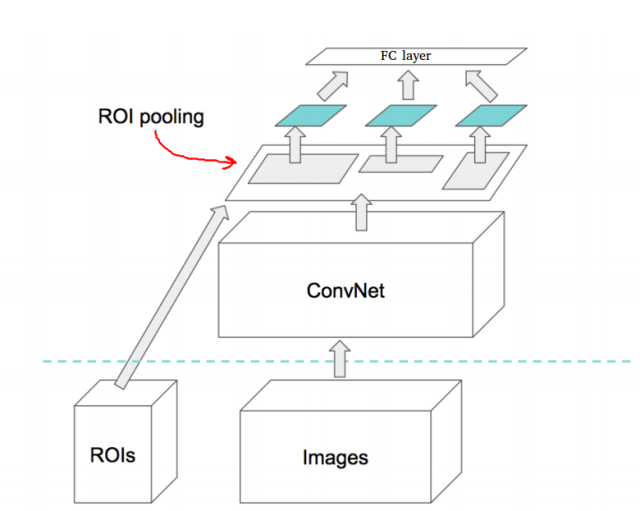
\includegraphics[width=0.6\columnwidth]{images/chap2/RoiPoolingLayer.png}
    \footcaption{Roi Pooling layer dùng để resize các proposals}
    \label{chap2:2.34}
    \end{figure}
\end{center}
\footnotetext{Nguồn: \url{http://cs231n.stanford.edu/slides/2016/winter1516_lecture8.pdf}}

Mô hình Fast R-CNN được huấn luyện theo các bước như sau:
\begin{enumerate}
    \item Sử dụng các mạng huấn luyện có sẵn
    \item Mô hình chỉ cần feed-forward một lần qua các lớp convolutional đối với ảnh đầu vào là đã thu được các features của nó.
    \item Tính toán vị trí của các features dựa vào kích thước và vị trí của các proposals đối với ảnh gốc để đưa ra các RoI 
    \item Dự đoán tọa độ các đỉnh của bounding box và vật thể nằm trong nó bằng các feature trong proposal.
\end{enumerate}

Đối với Fast R-CNN, do chia sẻ tính toán giữa các region trong ảnh, tốc độ thực thi của giải thuật đã được giảm đáng kể. Phần tốn nhiều chi phí nhất chính là phần đưa ra các region proposals đầu vào.

\begin{center}
    \begin{figure}[htp]
    \centering
    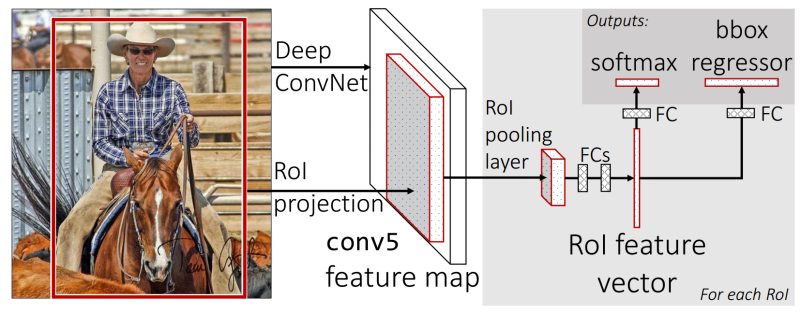
\includegraphics[width=0.5\columnwidth]{images/chap2/Fast_RCNN.png}
    \footcaption{Quá trình huấn luyện theo Fast R-CNN: hình ảnh đầu vào được đưa qua CNN huấn luyện sẵn để tạo thành feature map, các region proposals được xác định trên feature map để đưa ra các RoI, sau đó tiến hành phân loại và xác định bounding box từ các RoI đó}
    \label{fig:2.35}
    \end{figure}
\end{center}
\footnotetext{Nguồn: \cite{girshick2015fast}}
\subsubsection{Lớp RoI Pooling}
Lớp RoI Pooling dùng max pooling để chuyển những đặc trưng trong mỗi RoI trở thành một feature map nhỏ với một không gian 2 chiều cố định $h \times w$, với h và w là những hyper-parameter không phụ thuộc vào kích cỡ của RoI \cite{girshick2015fast}.

Lớp RoI Pooling hoạt động bằng cách chia RoI window với $h \times w$ thành  $H \times W$ ô sub-windows với kích thước xấp xỉ $H\mathbin{/}h \times W\mathbin{/}w$ và sau đó sử dụng max pooling giá trị ở mỗi sub-window để cho ra kích thước $h \times w$.

Hình \ref{chap2:cat1}, \ref{chap2:cat2}, \ref{chap2:cat3}, \ref{chap2:cat4} lần lượt là các bước hoạt động của RoI Pooling.
\begin{center}
    \begin{figure}[H]
    \centering
    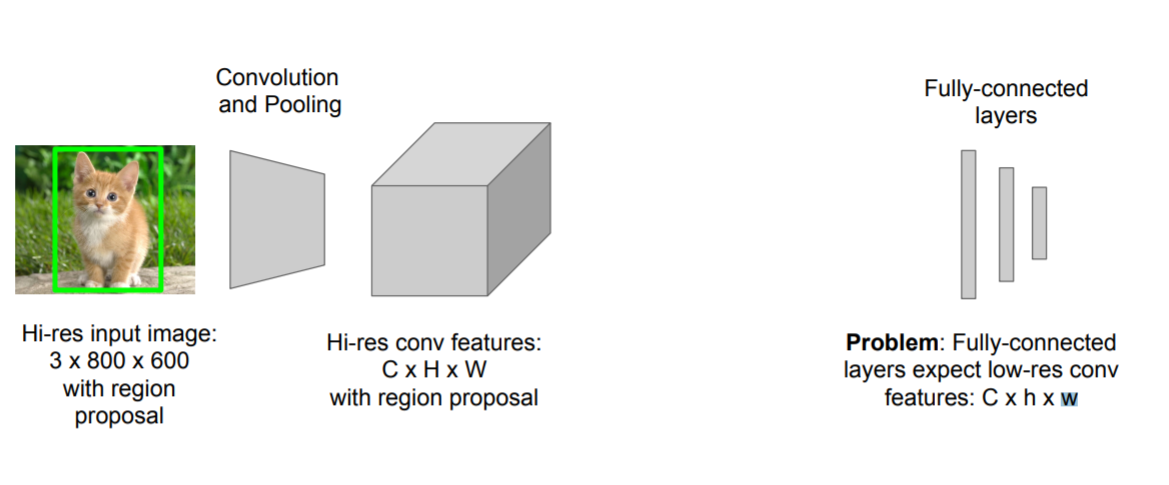
\includegraphics[width=0.8\columnwidth]{images/chap2/fastRCNN_1.png}
    \footcaption{Region Proposal được xác định}
    \label{chap2:cat1}
    \end{figure}
    \footnotetext{Nguồn: \url{http://cs231n.stanford.edu/slides/2016/winter1516_lecture8.pdf}}
\end{center}
\footnotetext{Nguồn: \url{http://cs231n.stanford.edu/slides/2016/winter1516_lecture8.pdf}}
\begin{center}
    \begin{figure}[H]
    \centering
    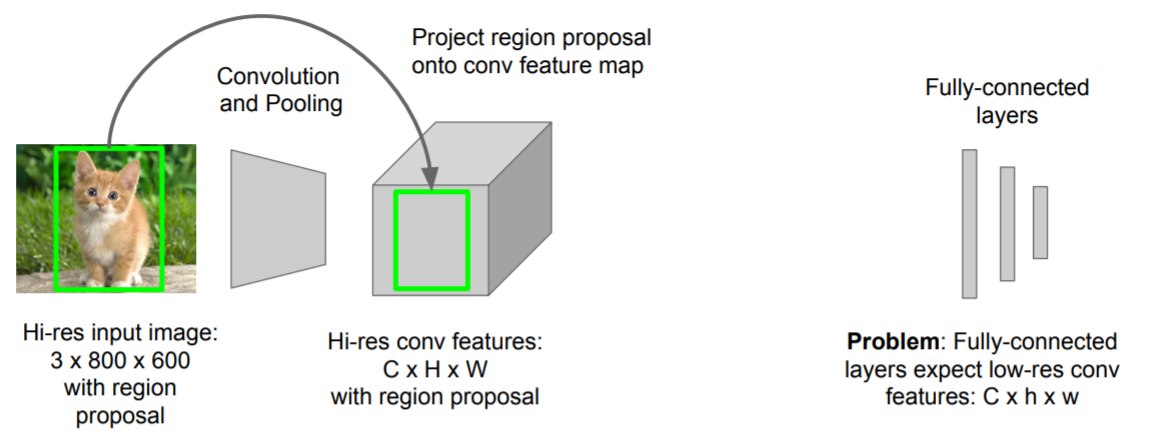
\includegraphics[width=0.8\columnwidth]{images/chap2/fastRCNN_2.png}
    \footcaption{Xác định Region Proposal trên feature map}
    \label{chap2:cat2}
    \end{figure}
\end{center}
\footnotetext{Nguồn: \url{http://cs231n.stanford.edu/slides/2016/winter1516_lecture8.pdf}}
\begin{center}
    \begin{figure}[H]
    \centering
    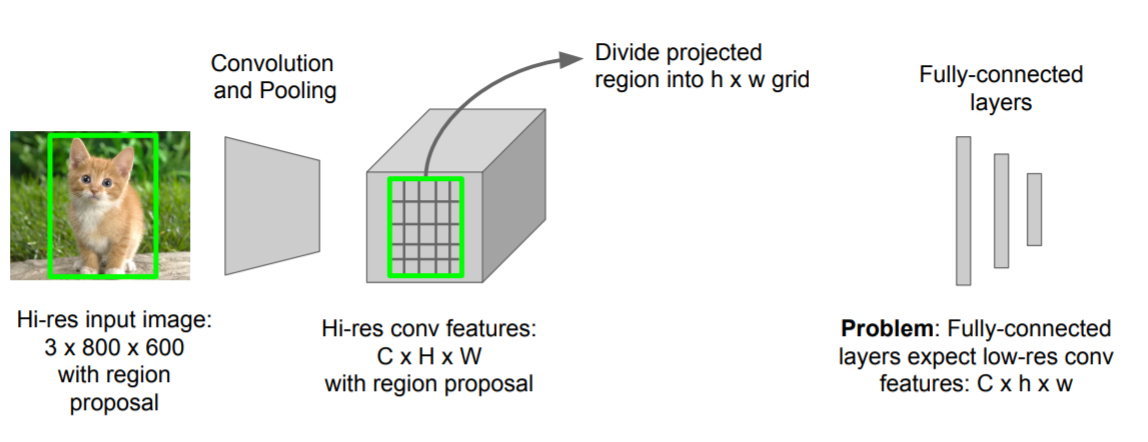
\includegraphics[width=0.8\columnwidth]{images/chap2/fastRCNN_3.png}
    \footcaption{Chia RoI window $H \times W$ xuống cỡ $h \times w$}
    \label{chap2:cat3}
    \end{figure}
\end{center}
\footnotetext{Nguồn: \url{http://cs231n.stanford.edu/slides/2016/winter1516_lecture8.pdf}}
\begin{center}
    \begin{figure}[H]
    \centering
    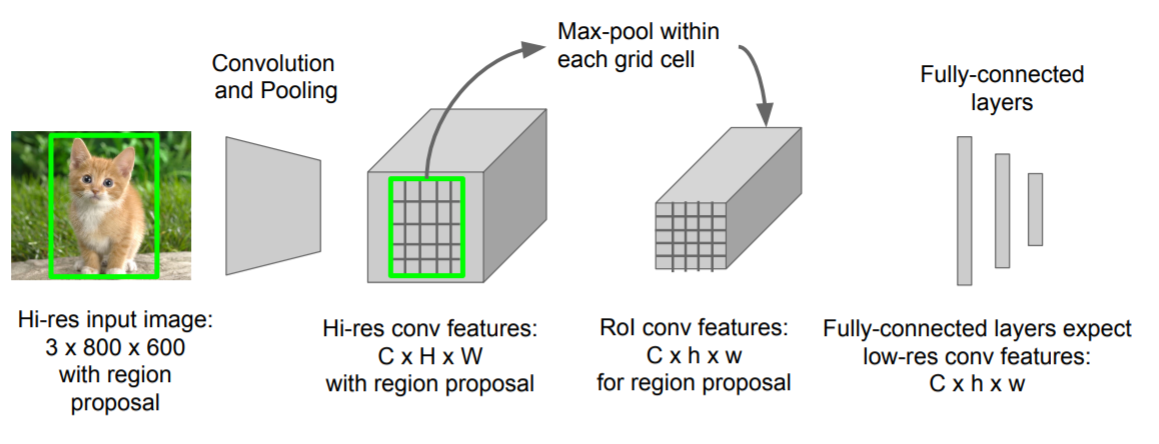
\includegraphics[width=0.8\columnwidth]{images/chap2/fastRCNN_4.png}
    \footcaption{Thực hiện max pooling}
    \label{chap2:cat4}
    \end{figure}
\end{center}
\footnotetext{Nguồn: \url{http://cs231n.stanford.edu/slides/2016/winter1516_lecture8.pdf}}
\subsubsection{Các hàm lỗi}
Fast R-CNN có hai lớp output đó là lớp tính xác suất phân bố $\mathbin{p} = (p_0, ..., p_K)$ trên mỗi RoI, với $K + 1$ loại. Thông thường xác suất $p$ sẽ được tính bởi hàm softmax thông qua $\mathbin{K} + 1$  outputs của lớp fully-connected. Lớp output thứ hai sẽ cho các thông số hồi quy của bounding box, $t^k = (t_x^k, t_y^k, t_w^k, t_h^k)$ với $\mathbin{k}$ là số chỉ mục của vật thể, $x, y, w, h$ lần lượt là tọa độ trục x, y, chiều dài, chiều cao của bounding box.

Trong quá trình huấn luyện, mỗi RoI đều được gán nhãn với một lớp ground-truth $\mathbin{u}$ và một ground-truth bounding-box $v$. Hàm lỗi $L$ cho mỗi RoI đã gán nhãn được xác định như sau:
\begin{center}
\begin{equation}
	L(p, u, t^u, v) = L_{cls}(p, u) + \lambda[u\geq 1]{L_{loc}}(t^u, v),
\end{equation}
\end{center}
Trong đó: 

$L_{cls}(p, u) = -\log p_u$ là log loss của class true $u$.

$p$ là xác suất phân bố của K + 1 classes

$u$ là ground-truth class $u$

$v$ là tọa độ ground-truth box

$t^u$ là tọa độ của bounding box thuộc class $u$

$L_{cls}$ là hàm lỗi của classifier

$L_{loc}$ là hàm lỗi của regressor

~\\
Hàm lỗi ${L_{loc}}$ được đặc tả qua bounding box true $v = (v_x, v_y, v_w, v_h)$ và kết quả dự đoán $t^u = (t_x^u, t_y^u, t_w^u, t_h^u)$. Điều kiện $[u\geq 1]$ bằng 1 khi $u \geq 1$ và bằng 0 nếu ngược lại, ý nghĩa của nó là nếu loại u có chỉ mục là 0 (là vùng nền, không chứa vật thể) thì sẽ không cần học vị trí của nó. \\
Tham số $\lambda$ được sử dụng để giữ cân bằng giữa hai hàm lỗi. Thông thường $\lambda$ sẽ có giá trị là 1.
Công thức hồi quy để tìm bounding box:
\begin{center}
\begin{equation}
	L_{loc}(t^u, v) = \sum_{i\in \{ x,y,w,h \}}smooth_{L_1}(t_i^u - v_i),
\end{equation}
\end{center}	
\begin{center}
\begin{equation}
    \text{với } smooth_{L_1}(x)=
    \begin{cases}
      0.5x^2, & \text{nếu}\ |a| < 1 \\
      |x| - 0.5, & \text{ngược lại,}
    \end{cases}
  \end{equation}
\end{center}
Hàm lỗi $L_1$ ít bị ảnh hưởng bởi các outliers hơn hàm lỗi $L_2$ được dùng trong mô hình R-CNN. Việc huấn luyện với hàm lỗi $L2$ cần phải chọn lọc tham số và learning rate một cách kĩ lưỡng để tránh việc gradients bị sai.
\subsection{Faster R-CNN}
Mặc dù đã được cải tiến nhiều nhưng Fast R-CNN vẫn còn một khuyết điểm rất lớn đó chính là sử dụng một mô hình thuật toán khác (selective search) để tìm ra các region proposals, việc này tạo ra hiệu ứng thắt cổ chai vì quá trình tìm kiếm các region proposals này diễn ra còn khá chậm. Vì thế mô hình Faster R-CNN tiếp tục được đưa ra giải quyết được khuyết điểm về thời gian thực thi của hai giải thuật trên bằng cách huấn luyện một mô hình hiệu quả hơn và thay thế vai trò của các thuật toán như Selective Search vốn rất chậm chạp.

Ý tưởng chính của giải thuật là dùng lớp Convolutional cuối cùng để dự đoán region proposals thay cho giải thuật selective search của mô hình Fast R-CNN cũ. Dựa vào hình \ref{faster_rcnn}, Faster R-CNN bao gồm hai modules:
\begin{enumerate}
    \item RPN (Region Proposals Network): đưa ra tập hợp các proposals dựa vào lớp Convolutional cuối cùng
    \item Fast R-CNN Roi Pooling: Phân loại và xác định vị trí từng proposals.
\end{enumerate}
\begin{center}
    \begin{figure}[H]
    \centering
    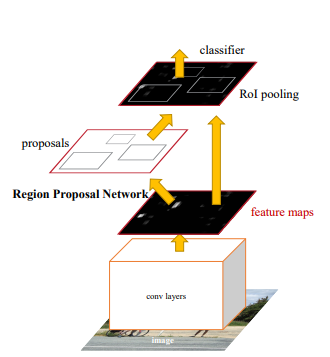
\includegraphics[width=0.7\columnwidth]{images/chap2/Faster_Rcnn_1.png}
    \footcaption{Quá trình huấn luyện theo Faster R-CNN}
    \label{chap2:faster_rcnn}
    \end{figure}
\end{center}
\footnotetext{Nguồn: \cite{ren2015faster}}
\subsubsection{Region Proposals Network}
Region Proposals Network lấy một hình với kích thước bất kì làm dữ liệu đầu vào và trả ra một tập tọa độ các proposals, với region là một khung hình chữ nhật.

Cách tạo ra các region proposals là cho trượt một sliding window (hình \ref{chap2:sliding_window}) nhỏ (một mô hình mạng nhỏ) $n \times n$ trên feature map. Sliding window này sẽ chuyển dữ liệu đầu vào thành những feature có kích thước rất nhỏ, thường là $1 \times 1$. Những feature này sẽ được đưa vào hai lớp fully-connected khác nhau. Một lớp là classifier dùng để phân loại đồng thời tính ra xác suất loại đó của feature đưa vào. Lớp còn lại là một regressor để tìm ra tọa độ bounding box.
\begin{center}
	\begin{figure}[H]
	\centering
	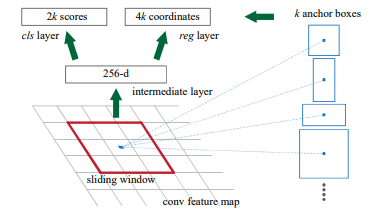
\includegraphics[width=0.7\columnwidth]{images/chap2/rpn.png}
    \footcaption{Sliding window}
    \label{chap2:sliding_window}
	\end{figure}
\end{center}
\footnotetext{Nguồn: \cite{ren2015faster}}

Ở mỗi vị trí của sliding window, giả sử có $k$ proposal được tìm thấy, khi đó regressor sẽ có $4k$ dữ liệu được xuất ra, tương ứng cho 4 tọa độ cho mỗi bounding box của proposal. Mỗi classifier cho hai loại score, một loại dự đoán xác suất cho trường hợp có vật và loại còn lại thì ngược lại. Những cái $k$ proposal được đề cập ở trên được gọi là anchors. Thường thì sẽ có 9 anchors  gồm hình tứ giác có 3 tỉ lệ với 3 kích thước khác nhau cho mỗi cho mỗi vị trí của sliding window trong feature map. Các anchor này sẽ được phân loại là có chứa vật hoặc không dựa trên tỉ lệ Intersection over Union sẽ được trình bày ở phần sau. Nếu tỉ lệ IoU này lớn hơn 0.7 thì anchor sẽ được cho là có chứa vật, ngược lại nếu IoU nhỏ hơn 0.3 thì anchor sẽ được cho là không chứa vật. Nếu 0.3 < IoU < 0.7 thì anchor đó sẽ được bỏ qua. Phương pháp này gọi là Non-Max Suppression. Dựa vào những anchor này, mô hình có thể có được xác suất chứa vật của mỗi region proposal tương ứng với một anchor đến ground-truth box tương ứng để xác định vị trí của bounding box.

Hàm lỗi:
\begin{center}
	\begin{equation}
		L(\{p_i\},\{y_i\}) = \frac{1}{N_{cls}}\sum_{i}L_{cls}(p_i, p_i^{*}) + \lambda \frac{1}{N_{reg}} \sum_{i}p_i^{*}L_{reg}(t_i, t_i^{*})
	\end{equation}
\end{center}
Trong đó:

$i$ là chỉ mục của anchor trong mini-batch

$p_i$ là xác suất dự đoán anchor thứ $i$ là vật thể

giá trị của ground-truth $p_i^*$ là 1 hoặc 0

$t_i$ là tọa độ bounding box dự đoán của anchor thứ $i$

$t_i^*$ là tọa độ ground-truth box
~\\
Các hyper-parameter $N_{cls}$, $N_{reg}$ và $\lambda$được dùng để chuẩn hóa lại công thức hàm lỗi trên. Theo bài báo \cite{ren2015faster}, $N_{cls}$ có giá trị bằng với kích thước của mini-batch và $N_{reg}$ được xấp xỉ bằng số lượng anchor chạy trên feature map.

\subsubsection{Huấn luyện Regional Proposals Network}
\begin{enumerate}
    \item Chọn một mạng CNN đã được train
    \item Từ layer Convolutional cuối cùng, ta được feature maps (hình \ref{chap2:last_convo})
    \begin{center}
    \begin{figure}[H]
    \centering
    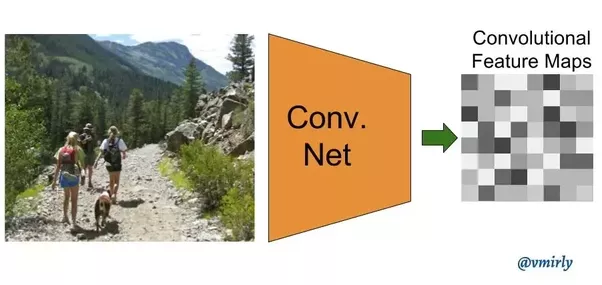
\includegraphics[width=0.7\columnwidth]{images/chap2/step-1.png}
    \footcaption{Feed-forward ảnh đầu vào thu được các features}
    \label{chap2:last_convo}
    \end{figure}
    \end{center}
    \footnotetext{Nguồn: \url{https://www.quora.com/How-does-the-region-proposal-network-RPN-in-Faster-R-CNN-work}}
    \item Với feature có được ở bước trước, ta dùng một sliding window, với mỗi bước trượt, ta tạo k anchors (trong hình \ref{chap2:anchor_9} là 9), với các tỉ lệ đa dạng (hình vuông, $1 \times 2$, $2 \times 1$, ...)\\
    \begin{center}
    \begin{figure}[H]
    \centering
    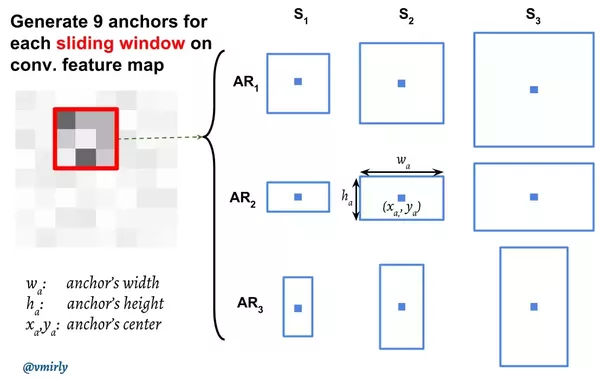
\includegraphics[width=0.7\columnwidth]{images/chap2/step-2.png}
    \footcaption{Tạo 9 anchors với từng sliding window }
    \label{chap2:anchor_9}
    \end{figure}
    \end{center}
    \footnotetext{Nguồn: \url{https://www.quora.com/How-does-the-region-proposal-network-RPN-in-Faster-R-CNN-work}}
    \item Huấn luyện một RPN với đầu vào là output của bước 3 có hai tác dụng chính: dự đoán tọa độ của bounding box và dự đoán bounding box đó có chứa vật thể hay không. Hình \ref{chap2:good_anchor} là một ví dụ về các anchors cho kết quả khá tốt
    \begin{center}
    \begin{figure}[H]
    \centering
    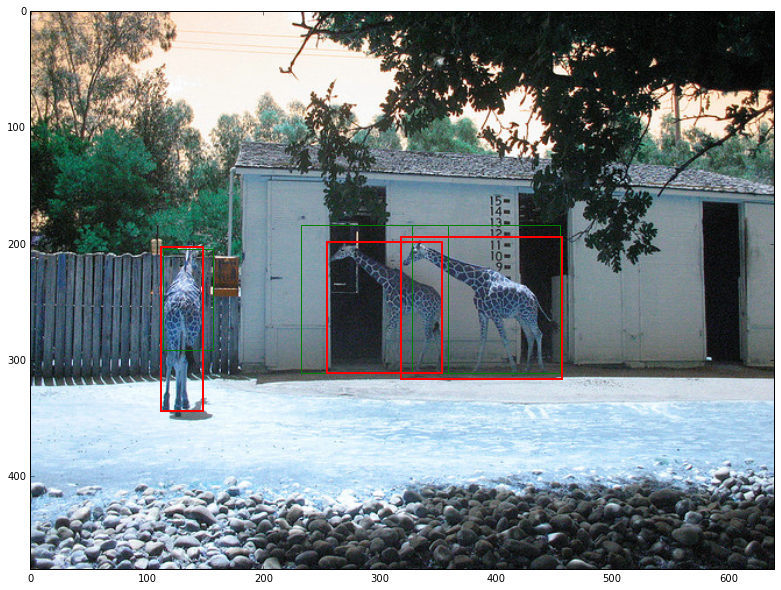
\includegraphics[width=0.7\columnwidth]{images/chap2/index.png}
    \footcaption{Những anchor có overlap khá tôt. Màu đỏ là ground truth boxes, màu xanh là anchor được tạo ra }
    \label{chap2:good_anchor}
    \end{figure}
    \end{center}
    \footnotetext{Nguồn: \url{https://www.quora.com/How-does-the-region-proposal-network-RPN-in-Faster-R-CNN-work}}
\end{enumerate}
\subsubsection{Mô hình mạng Faster R-CNN}
\begin{center}
    \begin{figure}[H]
    \centering
    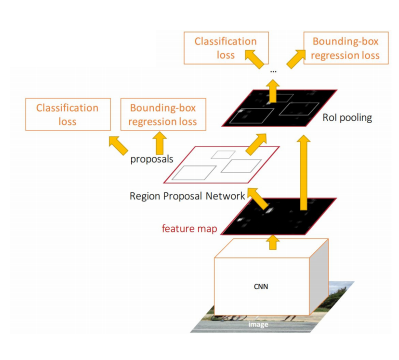
\includegraphics[width=0.7\columnwidth]{images/chap2/Faster_Rcnn_3.png}
    \footcaption{Mô hình huấn luyện Faster R-CNN}
    \label{chap2:faster_rcnn}
    \end{figure}
\end{center}
\footnotetext{\cite{ren2015faster}}
Nhờ lớp RPN, mô hình giải thuật Faster R-CNN trở nên nhanh hơn vì không còn bị thắt nút chai do phải dùng giải thụật khác để tìm ra các proposals. Các proposal này cùng với feature map được đưa vào quá trình RoI Pooling áp dụng theo giải thuật Fast R-CNN (hình \ref{chap2:faster_rcnn}), vậy mô hình Faster R-CNN gồm có tổng cộng 4 hàm lỗi:
\begin{itemize}
	\item Lỗi RPN classification
	\item Lỗi RPN regression
	\item Lỗi Fast R-CNN classification
	\item Lỗi Fast R-CNN regression
\end{itemize}
\section{Các phương pháp kiểm tra}
\subsection{Intersection over Union}
Trong bài toán nhận diện vật thể sử dụng 4 tọa độ để xác định bounding box, Intersection over Union (IoU) là một phương pháp thường được áp dụng để xét xem vật thể nhận diện được đã đúng với dữ liệu đươc gán nhãn chưa. Cần có hai cặp tọa độ để áp dụng phương pháp này, đó là tọa độ của bounding box nhận diện được và tọa độ của ground-truth box được gán nhãn sẵn một cách thủ công, thường bởi con người, dùng để kiểm tra vị trí của bounding box nhận diện được đã chính xác chưa.

Trong thực tế đối với vấn đề nhận diện ảnh, rất khó để có phương pháp so sánh trực tiếp các tọa độ $(x, y)$ nhận diện được trong ảnh bởi thuật toán xem có trùng với các tọa độ $(x, y)$ trong ground-truth box hay không. Do đó kĩ thuật đánh giá dựa trên sự chồng lên nhau (overlapping) được đề xướng và áp dụng thực tiễn.

Công thức tính IoU:

\begin{center}
	\begin{equation}
		IoU = \frac{\text{diện tích } \text{bounding box } \cap \text{ground-truth box}}{\text{diện tích } \text{bounding box } \cup \text{ground-truth box}}
	\end{equation}
\end{center}

IoU thường được tính bằng tỉ lệ diện tích vùng giao (intersection) giữa bounding box với ground-truth box so với diện tích vùng hợp (union) giữa ground-truth box và bounding box (hình \ref{chap2:iou_cal}). Từ đó ta có thể thấy được tỉ lệ chồng lên nhau của hai box.

\begin{center}
\begin{figure}[H]
    \centering
    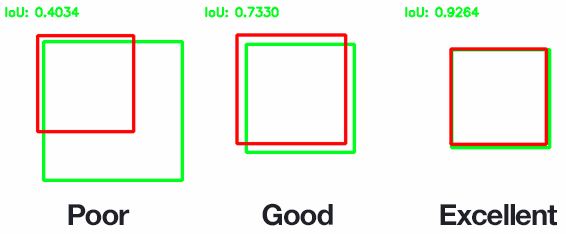
\includegraphics[width=0.7\columnwidth]{images/chap2/iou.png}
    \footcaption{Ví dụ về kĩ thuật đánh giá áp dụng IoU}
    \label{chap2:iou_cal}
    \end{figure}
\end{center}
\footnotetext{Nguồn: https://www.pyimagesearch.com/2016/11/07/intersection-over-union-iou-for-object-detection/}

Với những kết quả bounding box nhận diện được chồng nhiều lên ground-truth box thì IoU sẽ có giá trị cao và ngược lại, nếu kết quả bounding box quá nhỏ hay quá lớn so với ground-truth box thì IoU sẽ có giá trị thấp.

\subsection{Image matching}
Đây là phương pháp so sánh vật thể nhận diện được trong ảnh với vật thể đã gán nhãn của chính ảnh đó để đánh giá độ chính xác của giải thuật.\\
Theo \cite{szeliski2010computer}:
\begin{itemize}
	\item TP: True Positive
	
	Là những trường hợp vật thể được nhận diện đúng với vật thể được gán nhãn.
	\item FN: False Negative
	
	Là những trường hợp không nhận diện được vật thể nhưng vật thể đó được gán nhãn.	
	\item FP: False Positive
	
	Là những trường hợp nhận diện được vật thể nhưng vật thể đó không có thực trong nhãn.
	\item TN: True Negative
	
	Là những trường hợp không nhận diện được vật thể và vật thể không có thực trong nhãn.
\end{itemize}
\subsection{Precision và recall}
Công thức của precision và recall như sau:
\begin{center}
	\begin{equation}
		Precision = \frac{\text{true positives}}{\text{true positives } + \text{ false positives}}
	\end{equation}
\end{center}
\begin{center}
	\begin{equation}
		Recall = \frac{\text{true positives}}{\text{true positives } + \text{ false negatives}}
	\end{equation}
\end{center}
Precision được xem là thước đo để đánh giá độ chính xác của những khẳng định từ giải thuật. $TP + FP$ là tất cả những trường hợp giải thuật cho kết quả là positive, đối với bài toán nhận diện vật thể thì nó có nghĩa là tất cả các trường hợp giải thuật nhận diện là có vật thể. Vậy precision đại diện cho tỉ lệ chính xác của những phán đoán của giải thuật cho rằng vị trí nào có vật thể. Ví dụ Precision có giá trị là 0.8, mà thuật toán tìm được 5 vị trí có vật thể, vậy có nghĩa là có 4 vị trí là chính xác so với dữ liệu gán nhãn.

Recall thì được xem là thước đo để đánh giá độ chính xác so với dữ liệu được gán nhãn. $TP + FN$ là tất cả những trường hợp được gán nhãn là positive. Độ đo này chủ yếu để xác định độ chính xác hoặc sự tìm ra đầy đủ của giải thuật. Điều này áp dụng vào bài toán nhận diện vật thể có nghĩa là recall giúp ta đánh giá xem một giải thuật có thật sự nhận diện đủ các mẫu được gán nhãn hay không.

Khi sử dụng hai tỉ lệ này để đánh giá độ chính xác cân phải xem xét sự phù hợp của bài toán, nếu quá thiên về precision thì recall sẽ thấp, có nghĩa là nếu quá tập trung vào việc mỗi vật dự đoán ra từ giải thuật phải chính xác thì sẽ có rất nhiều trường hợp bị thiếu và ngược lại nếu tập trung vào recall thì precision sẽ thấp, có nghĩa là nếu cứ tập trung quá vào việc nhận diện đủ các vật thể so với dữ liệu gán nhãn thì những vật bị nhận diện thừa sẽ tăng lên.


\cleardoublepage

\chapter{GIẢI PHÁP ĐỀ XUẤT}
\label{chap:caseFarming}
\paragraph{Chương 3} sẽ giới thiệu về giải pháp đề xuất của nhóm để giải quyết bài toán nhận diện trái trái bưởi.


\section{Phân tích}
Bài toán nhận diện và đếm vật thể là một vấn đề không xa lạ, đã có nhiều nghiên cứu chỉ ra lời giải cho bài toán này.
\subsection{Sử dụng phương pháp Segmentation}
Trong nghiên cứu của Cohen \cite{cohen2010estimation}, nhận diện các vật thể được giải quyết bằng phương pháp phân loại từng điểm ảnh (pixel), sau đó gom lại nhưng điểm ảnh có khả năng cao là vật thể và từ đó phân biệt từng vật thể với nhau.

Quá trình này tốn khá nhiều công sức, đồng thời chưa thể xây dựng một bộ nhận diện vật thể "end-to-end", mà phải qua nhiều quá trình huấn luyện khác nhau. Không những bất lợi như vậy, phương pháp này vân chưa hiệu quả khi lớp vật thể nhận diện có quá nhiều hình dạng và màu sắc khác nhau, đặc biệt là phương pháp này bị ảnh hưởng mạnh bởi độ sáng và bóng râm trong ảnh.

\subsection{Sử dụng YOLOv2}
Được giới thiệu gần đây, mô hình này có thể huấn luyện để phân loại và xác định vị trí vật thể với tốc độ nhanh và độ chính xác cao, YOLO được xem là một giải pháp để giải quyết bài toán nhận diện vật thể thời gian thực.

YOLO mặc dù có tốc độ huấn luyện và chạy mô hình nhanh nhưng YOLO sử dụng phương pháp chia hình đầu vào thành các ô để dự đoán kết quả ô đó có vật thể hay không nên mỗi ô chỉ có thể dự đoán được một lớp vật thể, việc này tạo nên những hạn chế rất lớn đối với bài toán nhận diện trái cây, đặc biệt là những trái nằm gần nhau.

Mô hình YOLO không sử dụng các đặc trưng được chuyển giao từ mô hình được huấn luyện sẵn, cho nên việc nhận diện đặc trưng mới, bất thường so với dữ liệu huấn luyện của YOLO chưa thực sự tốt.

\section{Giải pháp}
Để giải quyết bài toán, đặc biệt là vấn đề nhận diện được trái bưởi ở các loại ánh sáng, bóng râm và đồng thời phân biệt được những trái ở gần nhau, nhóm đã quyết định sử dụng mô hình Faster R-CNN.

Faster R-CNN không những giải quyết được vấn đề về màu sắc, độ sáng của các loại trái cây, bởi vì đặc trưng của nó được trích xuất từ những lớp mạng tích chập. Đồng thời những lớp mạng tích chập này được chuyển giao trọng số từ mạng VGG-16 nên khả năng trích xuất ra đặc trưng tốt. Không những vậy, nhờ mạng RPN được tích hợp trong nó đã giúp cho Faster R-CNN có thể phát hiện được những trái ở gần nhau, đồng thời biết được và loại bỏ những bounding box nào đang cùng đánh dấu một trái.

Nhược điểm của Faster R-CNN là chạy còn chưa thực sự nhanh (khoảng 0.3 giây một hình), tuy nhiên đối với bài toán cần giải của nhóm, việc chạy được giải thuật theo thời gian thực là chưa thực sự quá cần thiết.

Bên cạnh việc sử dụng giải thuật này, nhóm còn kết hợp với sử dụng threshold (ngưỡng) để đánh giá xem trái nhận diện được có thực sự là trái đúng không, đồng thời kết hợp với một bộ phân loại được xây dựng từ những lớp mạng tích chập để phân loại trái nhận diện được có thực sự là trái đúng hay là lá hoặc các vật thể khác.

\cleardoublepage

\chapter{ỨNG DỤNG FASTER R-CNN TRONG NHẬN DIỆN TRÁI BƯỞI}
\label{chap:caseMedical}
\paragraph{Chương 4} sẽ trình bày các công tác chuận bị, quá trình huấn luyện và kết quả thu được từ việc áp dụng Faster R-CNN vào bài toán nhận diện trái bưởi. Nhóm sẽ trình bày về quá trình lấy mẫu của tập dữ liệu mà nhóm sử dụng cho việc huấn luyện và đánh giá kết quả, các thông số huấn luyện và cách đánh giá, biểu đồ thu được từ việc áp dụng giải thuật. Ở quá trình huấn luyện và kết quả, nhóm sẽ trình bày hai mô hình được đánh giá cho độ chính xác cao nhất. \\
\section{Chuẩn bị dữ liệu}
Dữ liệu hình ảnh nhóm có được gồm hai phần:
\begin{itemize}
  \item Dữ liệu tổng hợp từ nhiều nguồn, gồm 47 tấm, nội dung hình chủ yếu tập trung chụp cận cảnh các trái bưởi và đặc biệt giống bưởi da xanh.
  	\begin{center}
    	\begin{figure}[H]
    	\centering
    	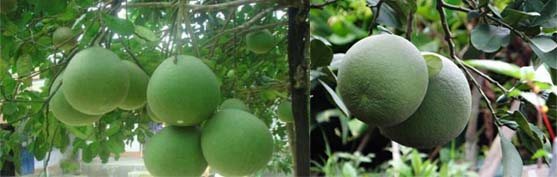
\includegraphics[width=0.8\columnwidth]{images/chap3/sample1.jpg}
    	\caption{Một vài ảnh mẫu trong tập dữ liệu đầu tiên}
    	\label{fig:my_label}
    	\end{figure}
	\end{center}
  \item Dữ liệu ảnh gồm 87 hình được chụp trực tiếp tại các vườn bưởi ở Bến Tre bằng máy ảnh kĩ thuật số. Hầu hết tất cả hình ảnh có được đều là giống bưởi da xanh và được chụp từ ngoài vào hoặc từ dưới gốc cây lên, sao cho trong ảnh vừa có cây, lá và quả. 
  	\begin{center}
    	\begin{figure}[H]
    	\centering
    	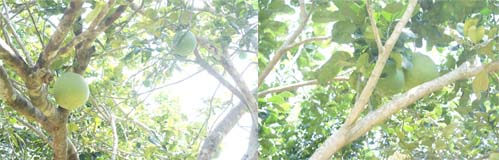
\includegraphics[width=0.7\columnwidth]{images/chap3/sample2.jpg}
    	\caption{Một vài ảnh mẫu trong tập dữ liệu thứ hai}
    	\label{fig:my_label}
    	\end{figure}
	\end{center}
Sau đó các ảnh được gán nhãn và thông qua thao tác augmentation để sinh ra tập ảnh gồm tổng cộng 10560 ảnh
\end{itemize}
\section{Tiền xử lí dữ liệu}
\subsection{Gán nhãn}
Từng trái bưởi trong các ảnh trong tập dữ liệu gốc được xác định vị trí và gán nhãn theo định dạng Pascal VOC để framework có thể đọc và thực thi (hình \ref{chap3:voc_format}).

Định dạng Pascal VOC được thể hiện dưới dạng file .xml gồm có cách trường sau:
\begin{itemize}
	\item folder
	\item filename
	\item path
	\item source
	\item size
	\begin{itemize}
		\item width
		\item height
		\item depth
	\end{itemize}
	\item segmented
	\item object
	\begin{itemize}
		\item name
		\item pose
		\item truncated 
		\item difficult
		\item bndbox
		\begin{itemize}
			\item xmin
			\item ymin
			\item xmax
			\item ymax
		\end{itemize}
	\end{itemize}
\end{itemize} 
Trong các trường trên, đối với phạm vi luận văn, ta quan tâm đến các trường size (gồm các trường width, height và depth) và object(bao gồm bndbox với các trường xmin, ymin, xmax, ymax bên trong), lần lượt là kích thước của bức ảnh đang xét và tọa độ, vị trí từng vật thể trong ảnh đó.
	\begin{center}
    	\begin{figure}[H]
    	\centering
    	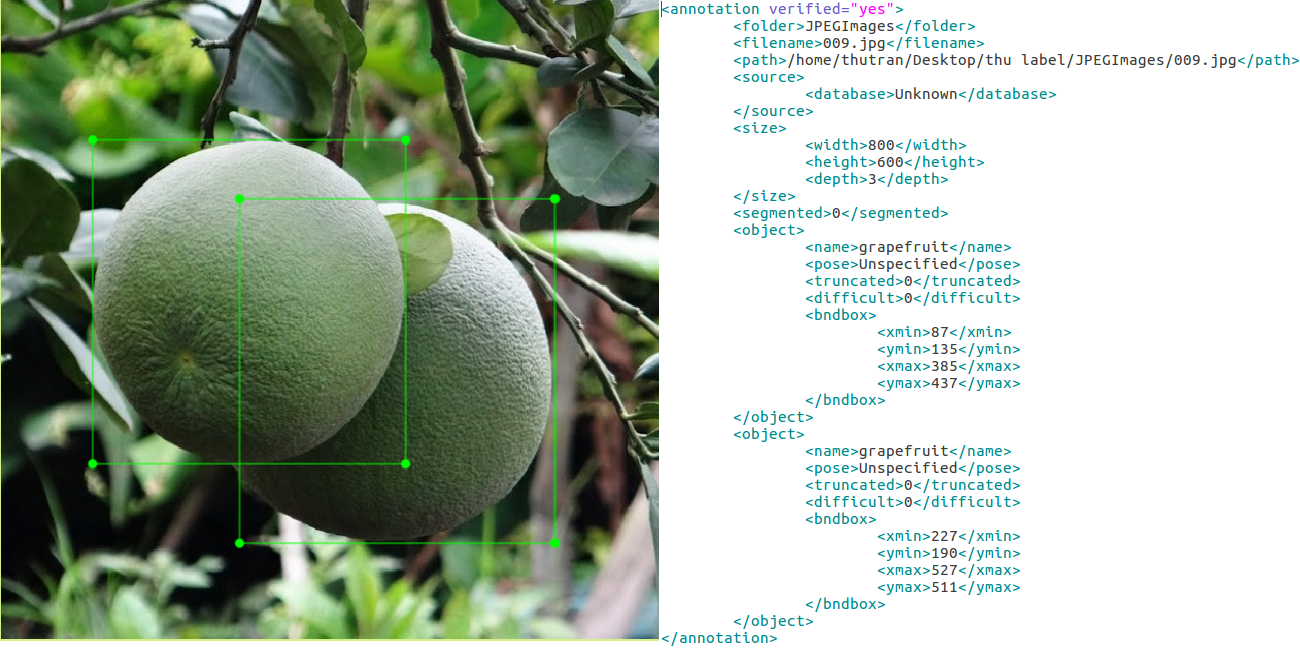
\includegraphics[width=0.7\columnwidth]{images/chap3/label.png}
    	\caption{Mỗi ảnh được mô tả bởi một file xml}
    	\label{chap3:voc_format}
    	\end{figure}
	\end{center}
Để hiện thực, ta sử dụng tool từ git sau:\\
\url{https://github.com/manhcuogntin4/Label-Annotation-VOC-Pascal} \\
Sau khi clone project về, chạy ứng dụng sẽ thấy giao diện như sau:
	\begin{center}
    	\begin{figure}[H]
    	\centering
    	\includegraphics[width=0.7\columnwidth]{images/chap3/UI1.png}
    	\caption{Giao diên tool Pascal VOC Annotation}
    	\label{fig:my_label}
    	\end{figure}
	\end{center}
Sau khi chọn ảnh trong tập dữ liệu và label, ta có giao diện sau:
	\begin{center}
    	\begin{figure}[H]
    	\centering
    	\includegraphics[width=0.7\columnwidth]{images/chap3/UI2.png}
    	\caption{Giao diên sau khi đã label}
    	\label{fig:my_label}
    	\end{figure}
	\end{center}
Để xuất file .xml, chọn Verify Image (hình \ref{chap3:verify}), file annotation sẽ được lưu cùng folder với file ảnh hoặc ở folder khác được setup trong Change Save Dir
	\begin{center}
    	\begin{figure}[H]
    	\centering
    	\includegraphics[width=0.7\columnwidth]{images/chap3/UI3.png}
    	\caption{Chọn Verify Image để xuất file xml}
    	\label{chap3:verify}
    	\end{figure}
	\end{center}
\cleardoublepage
Nội dung một file xml:
\begin{lstlisting}[language=XML]
<annotation verified="yes">
	<folder>JPEGImages</folder>
	<filename>001.jpg</filename>
	<path>/home/JPEGImages/001.jpg</path>
	<source>
		<database>Unknown</database>
	</source>
	<size>
		<width>640</width>
		<height>427</height>
		<depth>3</depth>
	</size>
	<segmented>0</segmented>
	<object>
		<name>grapefruit</name>
		<pose>Unspecified</pose>
		<truncated>0</truncated>
		<difficult>0</difficult>
		<bndbox>
			<xmin>290</xmin>
			<ymin>125</ymin>
			<xmax>441</xmax>
			<ymax>272</ymax>
		</bndbox>
	</object>
	<object>
		<name>grapefruit</name>
		<pose>Unspecified</pose>
		<truncated>0</truncated>
		<difficult>0</difficult>
		<bndbox>
			<xmin>42</xmin>
			<ymin>271</ymin>
			<xmax>135</xmax>
			<ymax>360</ymax>
		</bndbox>
	</object>
	<object>
		<name>grapefruit</name>
		<pose>Unspecified</pose>
		<truncated>0</truncated>
		<difficult>0</difficult>
		<bndbox>
			<xmin>373</xmin>
			<ymin>51</ymin>
			<xmax>459</xmax>
			<ymax>152</ymax>
		</bndbox>
	</object>
	<object>
		<name>grapefruit</name>
		<pose>Unspecified</pose>
		<truncated>0</truncated>
		<difficult>0</difficult>
		<bndbox>
			<xmin>236</xmin>
			<ymin>204</ymin>
			<xmax>310</xmax>
			<ymax>294</ymax>
		</bndbox>
	</object>
</annotation>
\end{lstlisting}
\subsection{Augmentation}
Data augmentation là một phương pháp rất phổ biến được dùng trong Học máy, đặc biệt là phân loại ảnh, dùng để tăng kích thước của tập dữ liệu, đồng thời tránh hiện tượng overfit.

Trong phạm vi luận văn, nhóm hiện thực các kĩ thuật cơ bản như tăng giảm độ sáng ảnh với 2 mức độ sáng và 2 mức độ tối, làm nhiễu, làm mờ, lật ảnh, xoay ảnh các góc 90, 180, 270 độ. Các thao tác augmentation được thực thi trên cả các bounding box đã được gán nhãn ở bước trước.

Sau đây là hình ảnh trước và sau khi augment của từng kĩ thuật:
	\begin{center}
    	\begin{figure}[H]
    	\centering
    	\includegraphics[width=0.6\columnwidth]{images/chap3/twerkLight.jpg}
    	\caption{Ảnh gốc đã được label và các mẫu sau khi điều chỉnh độ sáng}
    	\label{fig:my_label}
    	\end{figure}
	\end{center}
	\begin{center}
    	\begin{figure}[H]
    	\centering
    	\includegraphics[width=0.4\columnwidth]{images/chap3/twerkNoise.jpg}
    	\caption{Ảnh gốc đã được label và mẫu sau khi làm nhiễu}
    	\label{fig:my_label}
    	\end{figure}
	\end{center}
	\begin{center}
    	\begin{figure}[H]
    	\centering
    	\includegraphics[width=0.4\columnwidth]{images/chap3/twerkBlur.jpg}
    	\caption{Ảnh gốc đã được label và mẫu sau khi làm mờ}
    	\label{fig:my_label}
    	\end{figure}
	\end{center}
	\begin{center}
    	\begin{figure}[H]
    	\centering
    	\includegraphics[width=0.4\columnwidth]{images/chap3/twerkRef.jpg}
    	\caption{Ảnh gốc đã được label và mẫu sau khi lật}
    	\label{fig:my_label}
    	\end{figure}
	\end{center}
	\begin{center}
    	\begin{figure}[H]
    	\centering
    	\includegraphics[width=0.4\columnwidth]{images/chap3/twerkRotate.jpg}
    	\caption{Ảnh gốc đã được label và các mẫu sau khi xoay 90, 180, 270 độ}
    	\label{fig:my_label}
    	\end{figure}
	\end{center}
Với mỗi mẫu thu được  từ một kĩ thuật augmentation, ta lại áp dụng những kĩ thuật khác lên mẫu đó. Ví dụ, ta có thể làm mờ, làm nhiễu những ảnh đã được xoay. Nhờ đó từ một ảnh ta thu được khoảng 80 ảnh, tăng kích thước tập dữ liệu.
	\begin{center}
    	\begin{figure}[H]
    	\centering
    	\includegraphics[width=0.4\columnwidth]{images/chap3/augment.jpg}
    	\caption{Các mẫu thu được sau khi áp dụng tất cả kĩ thuật augmentation lên một ảnh}
    	\label{fig:my_label}
    	\end{figure}
	\end{center}

\section{Quá trình huấn luyện}
\subsection{Môi trường thực hiện}
Quá trình huấn luyện thí nghiệm được thực hiện trên máy tính sử dụng vi xử lí Intel Core i3-6100, 2 nhân 4 luồng với xung nhịp 3.70 GHz, bộ nhớ RAM có dung lượng là 8 Gb, kết hợp với GPU là GTX 1080. Hệ điều hành được sử dụng là Ubuntu Desktop 18.04. 
\subsection{Mã nguồn sử dụng}
Mã nguồn mà nhóm sử dụng là mã nguồn của mô hình giải thuật Faster R-CNN được công bố trên dịch vụ mã nguồn mở Github, được viết lại bằng ngôn ngữ python kết hợp với sử dụng thư viện Tensorflow của Google, mà nguồn này được tác giả của nó mô phỏng lại từ mã nguồn chính thức sử dụng thư viện Caffe. \\ \\
Link Github mã nguồn sử dụng thư viện Tensorflow: \\
\url{https://github.com/smallcorgi/Faster-RCNN_TF} \\
\\
Link Github mã nguồn sử dụng thư viện Caffe: \\
\url{https://github.com/rbgirshick/py-faster-rcnn} \\
\subsection{Định nghĩa một số khái niệm trong huấn luyện}
\begin{itemize}
	\item Batch là lượng dữ liệu huấn luyện được truyền đi trong môt lần đẩy dự liệu vào mạng nơ-ron để huấn luyện. Đối với giải thuật Faster R-CNN, batch thường có kích thước là 1, có nghĩa là mỗi lần chỉ đưa một bức ảnh vào để huấn luyện.  
	\item Iterations là số lần dữ liệu được đẩy đi (forward) và cập nhật ngược về (backward) với số lượng mẫu huấn luyện là kích thước của batch.
	\item Mỗi epoch là mỗi lần dữ liệu được đẩy đi và cập nhật ngược về với số lượng mẫu là cả tập huấn luyện.
	\item Lấy ví dụ như có tổng cộng 256 bức ảnh trong tập dữ liệu huấn luyện, với kích thước batch là 128 bức ảnh, vậy tức là mỗi một lần huấn luyện thêm một epoch sẽ tương đương với huấn luyện thêm 2 iterations.
\end{itemize}
\cleardoublepage
\subsection{Thiết kế mô hình}
Nhóm sử dụng lại nguyên bản mô hình của gốc của giải thuật Faster R-CNN (hình \ref{chap3:original_faster}) để có thể sử dụng được transfer learning từ bộ trọng số (weights) được trích xuất sẵn của VGG, điều này giúp cho việc học các đặc trưng mới nhanh hơn rất nhiều so với việc bắt đầu học mới từ đầu.
~\\
~\\
\begin{figure}[H]
  \centering
  \includegraphics[width=1\textwidth]{images/chap3/fasterRCNN.png}
  \footcaption{Mô hình gốc của giải thuật Faster R-CNN}
%  \caption{Biểu đồ lỗi case 1 ở bài toán Y khoa}
  \label{chap3:original_faster}    
\end{figure}
\footnotetext{Nguồn: \cite{sa2016deepfruits}}
%\subsection{Bộ thông số}
\subsection{Chiến lược huấn luyện}
\subsubsection{Trường hợp 1}
Ở trường hợp 1, nhóm tiến hành huấn luyện mô hình với learning rate là 0.001 ở 70000 iterations đầu tiên, sau đó nhóm cho hạ learning rate và tiếp tục huấn luyện 70000 iterations nữa rồi cho dừng. 
\subsubsection{Trường hợp 2}
Ở trường hợp 2, nhóm tiến hành huấn luyện mô hình với learning rate là 0.0001.
Sau khi huấn luyện được 70000 iterations, kết quả huấn luyện cho thấy quá trình huấn luyện bắt đầu bị overfitting, được thể hiện ở việc kết quả kiểm tra có độ chính xác (Average Precision) không tăng lên mà bắt đầu giảm xuống.
\cleardoublepage
\subsection{Hàm lỗi khi huấn luyện}
\subsubsection{Trường hợp 1}
\begin{center}
    \begin{figure}[H]
    \centering
    	\begin{subfigure}[H]{0.5\linewidth}
    		\centering
    		\includegraphics[width=\linewidth]{images/chap3/loss_box_2.png}
		    \caption{Biểu đồ loss box của trường hợp 1}
		    \label{fig:my_label}
		\end{subfigure}\hfill
		\begin{subfigure}[H]{0.5\linewidth}
    		\centering
    		\includegraphics[width=\linewidth]{images/chap3/loss_cls_2.png}
		    \caption{Biểu đồ loss classifier của trường hợp 1}
		    \label{fig:my_label}
		\end{subfigure}\hfill
	\caption{Biểu đồ loss box và loss classifier của trường hợp 1}
    \label{fig:mylabel}
    \end{figure}

    \begin{figure}[H]
    \centering
    	\begin{subfigure}[H]{0.5\linewidth}
    		\centering
    		\includegraphics[width=\linewidth]{images/chap3/rpn_loss_box_2.png}
		    \caption{Biểu đồ rpn loss box của trường hợp 1}
		    \label{fig:my_label}
		\end{subfigure}\hfill
		\begin{subfigure}[H]{0.5\linewidth}
    		\centering
    		\includegraphics[width=\linewidth]{images/chap3/rpn_loss_cls_2.png}
		    \caption{Biểu đồ rpn loss classifier của trường hợp 1}
		    \label{fig:my_label}
		\end{subfigure}\hfill
	\caption{Biểu đồ rpn loss box và rpn loss classifier của trường hợp 1}
    \label{fig:mylabel}
    \end{figure}

    \begin{figure}[H]
    \centering
    \includegraphics[width=0.9\columnwidth]{images/chap3/total_loss_2.png}
    \caption{Biểu đồ total loss của trường hợp 1}
    \label{fig:my_label}
    \end{figure}
\end{center}
\subsubsection{Trường hợp 2}
\begin{center}
	\begin{figure}[H]
    \centering
    	\begin{subfigure}[H]{0.5\linewidth}
    		\centering
    		\includegraphics[width=\linewidth]{images/chap3/Loss_Box.png}
		    \caption{Biểu đồ loss box của trường hợp 2}
		    \label{fig:my_label}
		\end{subfigure}\hfill
		\begin{subfigure}[H]{0.5\linewidth}
    		\centering
    		\includegraphics[width=\linewidth]{images/chap3/Loss_Classifier.png}
		    \caption{Biểu đồ loss classifier của trường hợp 2}
		    \label{fig:my_label}
		\end{subfigure}\hfill
	\caption{Biểu đồ loss box và loss classifier của trường hợp 2}
    \label{fig:mylabel}
    \end{figure}

	\begin{figure}[H]
    \centering
    	\begin{subfigure}[H]{0.5\linewidth}
    		\centering
    		\includegraphics[width=\linewidth]{images/chap3/RPN_Loss_Box.png}
		    \caption{Biểu đồ rpn loss box của trường hợp 2}
		    \label{fig:my_label}
		\end{subfigure}\hfill
		\begin{subfigure}[H]{0.5\linewidth}
    		\centering
    		\includegraphics[width=\linewidth]{images/chap3/RPN_Loss_Classifier.png}
		    \caption{Biểu đồ rpn loss classifier của trường hợp 2}
		    \label{fig:my_label}
		\end{subfigure}\hfill
	\caption{Biểu đồ rpn loss box và rpn loss classifier của trường hợp 2}
    \label{fig:mylabel}
    \end{figure}
\end{center}

\begin{center}
    \begin{figure}[H]
    \centering
    \includegraphics[width=0.9\columnwidth]{images/chap3/Total_Loss.png}
    \caption{Biểu đồ total loss của trường hợp 2}
    \label{fig:my_label}
    \end{figure}
\end{center}
\subsection{Kết quả toàn bộ tập test}
\subsubsection{Trường hợp 1}
\begin{center}
    \begin{figure}[H]
    \centering
    \includegraphics[width=0.9\columnwidth]{images/chap3/curve_2.png}
    \caption{Biểu đồ Precision - Recall từ kết quả kiểm tra của trường hợp 1 với toàn bộ tập test}
    \label{fig:my_label}
    \end{figure}
\end{center}
~\\
~\\
~\\
\begin{table}[H]
    \begin{tabular}{p{4cm}  p{2.5cm}  p{5.5cm} }    
    \hline		
	Tên & Giá trị & Giải thích \\
	\hline
	True Positive & 22011 & Số trái được nhận đúng \\
	False Positive & 3457  & Số trường hợp bị nhầm lẫn là trái \\
	False Negative & 1104 & Số trái mô hình chưa nhận diện được \\

    \hline
    Tổng & 23115 & Tổng số trái trong hình \\
    
    \hline
	Average Precision & 0.9068 \\
	\hline
	\end{tabular}
	\caption{Kết quả kiểm tra ở trường hợp 1 với toàn bộ tập test}
    \label{chap3:case1:table01}    
\end{table}
\begin{center}
    \begin{figure}[htp]
    \centering
    \includegraphics[width=0.9\columnwidth]{images/chap3/correlation_tp_140k.png}
    \caption{Biểu đồ tương quan từ kết quả kiểm tra của trường hợp 1 giữa TP và dữ liệu gán nhãn}
    \label{fig:my_label}
    \end{figure}
\end{center}
~\\
~\\
~\\
\begin{table}[H]
    \begin{tabular}{p{4cm}  p{2.5cm}  p{5.5cm} }
    \hline		
	Tên & Giá trị & Giải thích \\
	\hline
	\multicolumn{3}{c}{Phương trình tương quan \textbf{y = ax + b}} \\
	a & 0.91460185 & Hệ số góc \\
	b & 0.27461432 & Hệ số tự do \\
	\hline
	
	Diff & 624 & Số ảnh khác với kết quả gán nhãn \\
	Độ chính xác & 0.80303 &  Tỉ lệ số ảnh đúng trên tất cả ảnh\\
	\hline
	\end{tabular}
	\caption{Kết quả kiểm tra ở trường hợp 1 giữa TP và dữ liệu gán nhãn}
    \label{chap3:case2:table02}    
\end{table}
\subsubsection{Trường hợp 2}
\begin{center}
    \begin{figure}[H]
    \centering
    \includegraphics[width=0.9\columnwidth]{images/chap3/PR_curve.png}
    \caption{Biểu đồ Precision - Recall từ kết quả kiểm tra trường hợp 2 với toàn bộ tập test}
    \label{fig:my_label}
    \end{figure}
\end{center}
~\\
~\\
\begin{table}[H]
    \begin{tabular}{p{4cm}  p{2.5cm}  p{5.5cm} }
    \hline		
	Tên & Giá trị & Giải thích \\
	\hline
	True Positive & 21317 & Số trái được nhận đúng \\
	False Positive & 12405  & Số trường hợp bị nhầm lẫn là trái \\
	False Negative & 1798 & Số trái mô hình chưa nhận diện được \\

    \hline
    Tổng & 23115 & Tổng số trái trong hình \\
    
    \hline
	Average Precision & 0.8919\\
	\hline
	\end{tabular}
	\caption{Kết quả kiểm tra ở trường hợp 2 với toàn bộ tập test}
    \label{chap3:case2:table02}    
\end{table}
\begin{center}
    \begin{figure}[H]
    \centering
    \includegraphics[width=0.9\columnwidth]{images/chap3/correlation_tp_70k.png}
    \caption{Biểu đồ tương quan của trường hợp 2 giữa TP và dữ liệu gán nhãn}
    \label{fig:my_label}
    \end{figure}
\end{center}
~\\
~\\
\begin{table}[H]
    \begin{tabular}{p{4cm}  p{2.5cm}  p{5.5cm} }   
    \hline		
	Tên & Giá trị & Giải thích \\
	\hline
	\multicolumn{3}{c}{Phương trình tương quan \textbf{y = ax + b}} \\
	a & 0.86838905 & Hệ số góc \\
	b & 0.39273578 & Hệ số tự do \\
	\hline
	Diff & 920 & Số ảnh khác với kết quả gán nhãn \\
	Độ chính xác & 0.7095959 &  Tỉ lệ số ảnh đúng trên tất cả ảnh\\
	\hline
	\end{tabular}
	\caption{Kết quả kiểm tra ở trường hợp 2 giữa TP và dữ liệu gán nhãn}
    \label{chap3:case2:table02}    
\end{table}
\subsection{Kết quả 50 mẫu trong tập test}
\subsubsection{Trường hợp 1}
\begin{center}
    \begin{figure}[H]
    \centering
    \includegraphics[width=0.9\columnwidth]{images/chap3/50_curve_140k.png}
    \caption{Biểu đồ Precision - Recall từ kết quả kiểm tra của trường hợp 1 với 50 mẫu}
    \label{fig:my_label}
    \end{figure}
\end{center}
\begin{table}[H]
    \begin{tabular}{p{4cm}  p{2.5cm}  p{5.5cm} }
    \multicolumn{3}{l}{Kết quả kiểm tra của trường hợp 1 với 50 mẫu} \\    
    \hline		
	Tên & Giá trị & Giải thích \\
	\hline
	
	True Positive & 377 & Số trái được nhận đúng\\
	False Positive & 46  & Số trường hợp bị nhầm lẫn là trái \\
	False Negative & 26 & Số trái mô hình chưa nhận diện được \\

    \hline
    Tổng & 403 & Tổng số trái trong hình \\
    
    \hline
	Average Precision & 0.9068 \\
	\hline
	\end{tabular}
	\caption{Kết quả kiểm tra ở trường hợp 1 với 50 mẫu}
    \label{chap3:case1:table01}    
\end{table}
\begin{center}
    \begin{figure}[htp]
    \centering
    \includegraphics[width=0.9\columnwidth]{images/chap3/tp_140k.png}
    \caption{Biểu đồ tương quan từ kết quả kiểm tra của trường hợp 1 với 50 mẫu, giữa TP và dữ liệu gán nhãn}
    \label{fig:my_label}
    \end{figure}
\end{center}
~\\
~\\
\begin{table}[H]
    \begin{tabular}{p{4cm}  p{2.5cm}  p{5.5cm} }
    \hline		
	Tên & Giá trị & Giải thích \\
	\hline
	\multicolumn{3}{c}{Phương trình tương quan \textbf{y = ax + b}} \\
	a & 0.90638772 & Hệ số góc \\
	b & 0.23451492 & Hệ số tự do \\
	\hline
	Diff & 9 & Số ảnh khác với kết quả gán nhãn \\
	Độ chính xác & 0.82 &  Tỉ lệ số ảnh đúng trên tất cả ảnh\\
	\hline
	\end{tabular}
	\caption{Kết quả kiểm tra ở trường hợp 1 giữa TP và dữ liệu gán nhãn}
    \label{chap3:case2:table02}    
\end{table}
\begin{center}
    \begin{figure}[htp]
    \centering
    \includegraphics[width=0.9\columnwidth]{images/chap3/all_140k.png}
    \caption{Biểu đồ tương quan từ kết quả kiểm tra của trường hợp 1 với 50 mẫu , giữa các hình nhận diện được và dữ liệu gán nhãn}
    \label{fig:my_label}
    \end{figure}
\end{center}
\begin{table}[H]
    \begin{tabular}{p{4cm}  p{2.5cm}  p{5.5cm} }   
    \hline		
	Tên & Giá trị & Giải thích \\
	\hline
	\multicolumn{3}{c}{Phương trình tương quan \textbf{y = ax + b}} \\
	a & 0.92341594 & Hệ số góc \\
	b & 0.57726751 & Hệ số tự do \\
	\hline	
	Diff & 13 & Số ảnh khác với kết quả gán nhãn \\
	Độ chính xác & 0.74 &  Tỉ lệ số ảnh đúng trên tất cả ảnh\\
	\hline
	\end{tabular}
	\caption{Kết quả kiểm tra ở trường hợp 1 giữa các hình nhận diện được và dữ liệu gán nhãn}
    \label{chap3:case2:table02}    
\end{table}
\begin{table}[H]
    \begin{tabular}{p{2cm}  p{2cm}  p{2cm} p{4cm} p{2cm} }
    \hline		
	STT ảnh & TP & FP & Số object đếm được & Số label\\
	\hline
	   0   & 5  & 1  &     5     &   5   \\		\hline
   1   & 4  & 1  &     4     &   4   \\     \hline
   2   & 2  & 1  &     2     &   2   \\     \hline
   3   & 7  & 5  &     11    &   8   \\     \hline
   4   & 7  & 5  &     12    &   7   \\     \hline
   5   & 16 & 5  &     19    &   25  \\     \hline
   6   & 9  & 0  &     9     &   9   \\     \hline
   7   & 27 & 1  &     27    &   28  \\     \hline
   8   & 8  & 1  &     9     &   8   \\     \hline
   9   & 18 & 4  &     20    &   22  \\     \hline
   10  & 15 & 5  &     16    &   16  \\     \hline
   11  & 9  & 1  &     10    &   10  \\     \hline
   12  & 4  & 0  &     4     &   4   \\     \hline
   13  & 10 & 0  &     10    &   10  \\     \hline
   14  & 3  & 0  &     3     &   3   \\     \hline
   15  & 3  & 1  &     4     &   3   \\     \hline
   16  & 18 & 4  &     18    &   22  \\     \hline
   17  & 25 & 1  &     26    &   25  \\     \hline
   18  & 7  & 0  &     7     &   7   \\     \hline
   19  & 6  & 0  &     6     &   6   \\     \hline
   20  & 7  & 0  &     7     &   7   \\     \hline
   21  & 2  & 0  &     2     &   2   \\     \hline
   22  & 2  & 0  &     2     &   2   \\     \hline
   23  & 3  & 0  &     3     &   3   \\     \hline
   24  & 2  & 0  &     2     &   2   \\     \hline
   25  & 13 & 0  &     13    &   13  \\     \hline
	\end{tabular}
	\caption{Bảng số liệu đo được với 140k iters (1)}
    \label{chap3:case1:table01}    
\end{table}

\begin{table}[H]
    \begin{tabular}{p{2cm}  p{2cm}  p{2cm} p{4cm} p{2cm} }
    \hline		
	STT ảnh & TP & FP & Số object đếm được & Số label\\
	\hline
   26  & 3  & 0  &     3     &   3   \\     \hline
   27  & 1  & 0  &     1     &   1   \\     \hline
   28  & 2  & 0  &     2     &   2   \\     \hline
   29  & 7  & 1  &     7     &   7   \\     \hline
   30  & 3  & 0  &     3     &   3   \\     \hline
   31  & 3  & 0  &     3     &   3   \\     \hline
   32  & 27 & 0  &     27    &   28  \\     \hline
   33  & 8  & 0  &     8     &   8   \\     \hline
   34  & 2  & 0  &     2     &   2   \\     \hline
   35  & 2  & 0  &     2     &   2   \\     \hline
   36  & 8  & 0  &     8     &   8   \\     \hline
   37  & 4  & 1  &     5     &   4   \\     \hline
   38  & 9  & 1  &     9     &   9   \\     \hline
   39  & 2  & 5  &     7     &   6   \\     \hline
   40  & 4  & 0  &     4     &   4   \\     \hline
   41  & 3  & 2  &     3     &   3   \\     \hline
   42  & 8  & 0  &     8     &   8   \\     \hline
   43  & 1  & 0  &     1     &   1   \\     \hline
   44  & 3  & 0  &     3     &   3   \\     \hline
   45  & 1  & 0  &     1     &   1   \\     \hline
   46  & 8  & 0  &     8     &   8   \\     \hline
   47  & 2  & 0  &     2     &   2   \\     \hline
   48  & 1  & 0  &     1     &   1   \\     \hline
   49  & 33 & 0  &     32    &   33  \\     \hline


	\end{tabular}
	\caption{Bảng số liệu đo được với 140k iters (2)}
    \label{chap3:case1:table01}    
\end{table}

\subsubsection{Trường hợp 2}
\begin{center}
    \begin{figure}[H]
    \centering
    \includegraphics[width=0.9\columnwidth]{images/chap3/50_curve_70k.png}
    \caption{Biểu đồ Precision - Recall từ kết quả kiểm tra trường hợp 2 với 50 mẫu}
    \label{fig:my_label}
    \end{figure}
\end{center}
\begin{table}[H]
    \begin{tabular}{p{4cm}  p{2.5cm}  p{5.5cm} }
    \multicolumn{3}{l}{Kết quả kiểm tra của trường hợp 2 với 50 mẫu} \\    
    \hline		
	Tên & Giá trị & Giải thích \\
	\hline
	True Positive & 364 & Số trái được nhận đúng \\
	False Positive & 162  & Số trường hợp bị nhầm lẫn là trái \\
	False Negative & 39 & Số trái mô hình chưa nhận diện được \\
    \hline
    Tổng & 403 & Tổng số trái trong hình \\
    \hline
	Average Precision & 0.8850\\
	\hline
	\end{tabular}
	\caption{Kết quả kiểm tra ở trường hợp 2 với 50 mẫu}
    \label{chap3:case2:table02}    
\end{table}
\begin{center}
    \begin{figure}[H]
    \centering
    \includegraphics[width=0.9\columnwidth]{images/chap3/tp_70k.png}
    \caption{Biểu đồ tương quan của trường hợp 2 với 50 mẫu, giữa TP và dữ liệu gán nhãn}
    \label{fig:my_label}
    \end{figure}
\end{center}
\begin{table}[H]
    \begin{tabular}{p{4cm}  p{2.5cm}  p{5.5cm} }   
    \hline		
	Tên & Giá trị & Giải thích \\
	\hline
	\multicolumn{3}{c}{Phương trình tương quan \textbf{y = ax + b}} \\
	a & 0.85391164 & Hệ số góc \\
	b & 0.39747212 & Hệ số tự do \\
	\hline	
	Diff & 12 & Số ảnh khác với kết quả gán nhãn \\
	Độ chính xác & 0.76 &  Tỉ lệ số ảnh đúng trên tất cả ảnh\\
	\hline
	\end{tabular}
	\caption{Kết quả kiểm tra ở trường hợp 2 giữa TP và dữ liệu gán nhãn}
    \label{chap3:case2:table02}    
\end{table}
\begin{center}
    \begin{figure}[H]
    \centering
    \includegraphics[width=0.9\columnwidth]{images/chap3/all_70k.png}
    \caption{Biểu đồ tương quan của trường hợp 2 với 50 mẫu, giữa các hình nhận diện được và dữ liệu gán nhãn}
    \label{fig:my_label}
    \end{figure}
\end{center}
\begin{table}[H]
    \begin{tabular}{p{4cm}  p{2.5cm}  p{5.5cm} }   
    \hline		
	Tên & Giá trị & Giải thích \\
	\hline
	\multicolumn{3}{c}{Phương trình tương quan \textbf{y = ax + b}} \\
	a & 0.99495528 & Hệ số góc \\
	b & 0.86066041 & Hệ số tự do \\
	\hline
	Diff & 12 & Số ảnh khác với kết quả gán nhãn \\
	Độ chính xác & 0.48 &  Tỉ lệ số ảnh đúng trên tất cả ảnh\\
	\hline
	\end{tabular}
	\caption{Kết quả kiểm tra ở trường hợp 2 giữa các hình nhận diện được và dữ liệu gán nhãn}
    \label{chap3:case2:table02}    
\end{table}
\begin{table}[H]
    \begin{tabular}{p{2cm}  p{2cm}  p{2cm} p{4cm} p{2cm} }
    \hline		
	STT ảnh & TP & FP & Số object đếm được & Số label\\
	\hline
	0   & 5  & 1  &     5     &   5   \\		
	\hline
	1   & 4  & 3  &     5     &   4   \\     
	\hline
	2   & 2  & 2  &     2     &   2   \\     
	\hline
	3   & 8  & 7  &     10    &   8   \\     
	\hline
	4   & 5  & 13 &     12    &   7   \\     
	\hline
	5   & 17 & 24 &     30    &   25  \\     
	\hline
	6   & 9  & 0  &     9     &   9   \\     
	\hline
	7   & 27 & 0  &     27    &   28  \\     
	\hline
	8   & 8  & 0  &     8     &   8   \\     
	\hline
	9   & 14 & 17 &     24    &   22  \\     
	\hline
	10  & 13 & 15 &     18    &   16  \\     
	\hline
	11  & 10 & 5  &     11    &   10  \\     
	\hline
	12  & 4  & 1  &     5     &   4   \\     
	\hline
	13  & 8  & 2  &     10    &   10  \\     
	\hline
	14  & 3  & 0  &     3     &   3   \\     
	\hline
	15  & 3  & 2  &     4     &   3   \\     
	\hline
	16  & 15 & 18 &     23    &   22  \\     
	\hline
	17  & 22 & 7  &     25    &   25  \\     
	\hline
	18  & 7  & 1  &     8     &   7   \\     
	\hline
	19  & 6  & 0  &     6     &   6   \\     
	\hline
	20  & 7  & 2  &     8     &   7   \\     
	\hline
	21  & 2  & 1  &     3     &   2   \\     
	\hline
	22  & 2  & 0  &     2     &   2   \\     
	\hline
	23  & 2  & 2  &     4     &   3   \\     
	\hline
	24  & 2  & 1  &     3     &   2   \\     
	\hline
	25  & 13 & 1  &     13    &   13  \\     
	\end{tabular}
	\caption{Bảng số liệu đo được với 70k iters (1)}
    \label{chap3:case1:table01}    
\end{table}

\begin{table}[H]
    \begin{tabular}{p{2cm}  p{2cm}  p{2cm} p{4cm} p{2cm} }
    \hline		
	STT ảnh & TP & FP & Số object đếm được & Số label\\
	\hline
	26  & 3  & 0  &     3     &   3   \\     
	\hline
	27  & 1  & 3  &     3     &   1   \\     
	\hline
	28  & 2  & 0  &     2     &   2   \\     
	\hline
	29  & 7  & 0  &     7     &   7   \\     
	\hline
	30  & 3  & 0  &     3     &   3   \\     
	\hline
	31  & 3  & 0  &     3     &   3   \\     
	\hline
	32  & 27 & 0  &     26    &   28  \\     
	\hline
	33  & 8  & 1  &     8     &   8   \\     
	\hline
	34  & 2  & 1  &     2     &   2   \\     
	\hline
	35  & 2  & 1  &     2     &   2   \\     
	\hline
	36  & 8  & 0  &     8     &   8   \\     
	\hline
	37  & 4  & 1  &     5     &   4   \\     
	\hline
	38  & 9  & 5  &     12    &   9   \\     
	\hline
	39  & 4  & 10 &     12    &   6   \\     
	\hline
	40  & 4  & 1  &     5     &   4   \\     
	\hline
	41  & 3  & 3  &     4     &   3   \\     
	\hline
	42  & 8  & 0  &     8     &   8   \\     
	\hline
	43  & 1  & 2  &     2     &   1   \\     
	\hline
	44  & 3  & 3  &     4     &   3   \\     
	\hline
	45  & 1  & 0  &     1     &   1   \\     
	\hline
	46  & 8  & 1  &     8     &   8   \\     
	\hline
	47  & 2  & 1  &     2     &   2   \\     
	\hline
	48  & 1  & 2  &     3     &   1   \\     
	\hline
	49  & 32 & 2  &     33    &   33  \\     
	\hline

	\end{tabular}
	\caption{Bảng số liệu đo được với 70k iters (2)}
    \label{chap3:case1:table01}    
\end{table}
\subsection{Demo}
Hình \ref{chap3:good} cho kết quả rất tốt, nhận diện đủ số lượng đối với trường hợp vật thể có mặt trong ảnh rõ ràng và ít bị khuất.
\begin{center}
    \begin{figure}[H]
    \centering
    \includegraphics[width=0.6\columnwidth]{images/chap3/demo_001.jpg}
    \caption{Một số hình ảnh demo}
    \label{chap3:good}
    \end{figure}
\end{center}

Hình \ref{chap3:good1}, \ref{chap3:good2} cũng cho kết quả khá tốt trong trường hợp số lượng trái nhiều, rõ và bị khuất bởi lá ít. 
\begin{center}
    \begin{figure}[H]
    \centering
    \includegraphics[width=0.6\columnwidth]{images/chap3/demo_002.jpg}
    \caption{Một số hình ảnh demo}
    \label{chap3:good1}
    \end{figure}
\end{center}

\begin{center}
    \begin{figure}[H]
    \centering
    \includegraphics[width=0.6\columnwidth]{images/chap3/demo_004.jpg}
    \caption{Một số hình ảnh demo}
    \label{chap3:good2}
    \end{figure}
\end{center}
Đối với các hình bị làm mờ, nhiễu, và thay đổi độ sáng với các trái ở gần rõ và ít bị che, kết quả nhận diện vẫn tốt.
\begin{center}
    \begin{figure}[H]
    \centering
    \includegraphics[width=0.6\columnwidth]{images/chap3/demo_006.jpg}
    \caption{Kết quả nhận diện với hình ảnh bị làm mờ}
    \label{chap3:good4}
    \end{figure}
\end{center}
\begin{center}
    \begin{figure}[H]
    \centering
    \includegraphics[width=0.6\columnwidth]{images/chap3/demo_007.jpg}
    \caption{Kết quả nhận diện với hình ảnh bị nhiễu}
    \label{chap3:good5}
    \end{figure}
\end{center}

\begin{center}
    \begin{figure}[H]
    \centering
    \includegraphics[width=0.6\columnwidth]{images/chap3/demo_012.jpg}
    \caption{Kết quả nhận diện với hình ảnh bị thay đổi độ sáng}
    \label{chap3:good6}
    \end{figure}
\end{center}

Hình \ref{chap3:lack1}, \ref{chap3:lack2}, \ref{chap3:lack3} đối với trường hợp trái nằm cạnh vùng có nhiều lá, kết quả nhận diện vẫn rất khả quan, tuy nhiên vẫn còn một số vị trí bị nhận diện nhầm.

\begin{center}
    \begin{figure}[H]
    \centering
    \includegraphics[width=0.7\columnwidth]{images/chap3/demo_008.jpg}
    \caption{Tuy nằm gần nhiều lá những trái bưởi vẫn được nhận diện tốt}
    \label{chap3:lack1}
    \end{figure}
\end{center}
\begin{center}
    \begin{figure}[H]
    \centering
    \includegraphics[width=0.7\columnwidth]{images/chap3/demo_009.jpg}
    \caption{Phần tường bị nhận diện nhầm thành bưởi}
    \label{chap3:lack2}
    \end{figure}
\end{center}
\begin{center}
    \begin{figure}[H]
    \centering
    \includegraphics[width=0.7\columnwidth]{images/chap3/demo_010.jpg}
    \caption{Xuất hiện một ít vùng bị nhận diện trùng nhau khi trái bưởi quá nhỏ}
    \label{chap3:lack3}
    \end{figure}
\end{center}


\cleardoublepage

\chapter{KẾT LUẬN VÀ HƯỚNG PHÁT TRIỂN}
\label{conclusion}
\paragraph{Chương 5} sẽ trình bày kết quả của quá trình huấn luyện dữ liệu mà nhóm chuẩn bị với mô hình Faster R-CNN đồng thời tự đánh giá về những việc đã và chưa làm được của nhóm, từ đó đưa ra hướng phát triển cho đề tài.

\section{Kết quả}
Dựa trên kết quả thu được từ 2 tập dữ liệu đánh giá, ta có cái nhìn tổng quát về quá trình và kết quả huấn luyện như sau:
\begin{itemize}
	\item Đối với hình ảnh có những trái to, rõ ràng, mô hình mạng đã nhận diện được chính xác và khá đầy đủ
	\item Đối với những hình ảnh cây có quá nhiều lá, lá che phần lớn các trái, mô hình mạng nhận diện được đúng các trái, tuy nhiên vẫn còn nhận dư và nhận thiếu các trái
	\item Cần cải thiện đối với những trường hợp trái bị che bởi cành, lá dẫn đến không nhận diện được, đưa tới kết quả là thiếu trái, được thể hiện bởi False Negative
	\item Các trường hợp nhận nhầm các vùng cành là thành trái (False Positive) cũng rất đáng được quan tâm và cải thiện
\end{itemize}
Để giải quyết hai vấn đề trên, nhóm đã đề xuất hướng giải quyết là đưa những vùng nhận diện được là trái bưởi qua các một CNN để phân loại.
Nhóm đã chuẩn bị tập dữ liệu với 14496 hình dùng cho việc huấn luyện và 7248 hình dùng cho việc kiểm tra, với hai class là có trái và không trái.
\begin{center}
    \begin{figure}[H]
    \centering
    \includegraphics[width=0.7\columnwidth]{images/chap3/loss_cls_full.png}
    \caption{Biểu đồ lỗi khi huấn luyện CNN phân loại ảnh có trái bưởi}
    \label{fig:my_label}
    \end{figure}
\end{center}
Kết quả huấn luyện cho độ chính xác 0.991 đối với tập dữ liệu kiểm tra, tuy nhiên khi áp dụng vào bộ phân loại vẫn chưa cho được hiệu quả như nhóm mong muốn, việc phân loại sai còn khá nhiều.\\
Từ kết quả thực nghiệm, có thể thấy được rằng việc áp dụng mô hình Faster R-CNN cho bài toán nhận diện và đánh giá năng suất cây ăn trái ở Việt Nam là khả thi, tuy nhiên cần áp dụng thêm nhiều biện pháp trong quá trình tiền xử lí và huấn luyện, đồng thời cần lượng dữ liệu lớn hơn để giúp mô hình hoạt động hoàn hảo hơn.
\section{Kết luận}
\subsection{Những việc đã làm được}
\begin{itemize}
\item Tìm hiểu các tổng quát lí thuyết và các phương pháp áp dụng thị giác máy tính và xử lí ảnh để giải quyết bài toán và những nghiên cứu liên quan

\item Tìm hiểu về mô hình mạng nơ-ron nhân tạo ANN, lí thuyết, kiến trúc và cách hoạt động của nó

\item Tìm hiểu về mô hình mạng CNN, cấu tạo của các lớp convolutional, lớp pooling và các hàm kích hoạt thường được sử dụng để giải quyết bài toán với dữ liệu hình ảnh

\item Tìm hiểu và thực hiện quá trình lấy mẫu ảnh cho ảnh thực tế, tiền xử lý ảnh, , augmentation để đa dạng hóa tập ảnh gốc, nhằm giúp nâng cao độ chính xác cho mô hình mạng

\item Tiến hành tìm hiểu thư viện Tensorflow, chỉnh sửa mã nguồn để áp dụng vào bài toán nhận diện trái bưởi

\item Tiến hành các quá trình huấn luyện, chỉnh sửa lỗi phát sinh của mã nguồn

\item Tìm hiểu và thực hiện các công đoạn đánh giá kết quả huấn luyện, chọn những mô hình cho kết quả tốt nhất, từ đó xem xét tính khả thi để áp dụng vào thực tiễn

\item Xây dựng được mô hình nhận diện trái bưởi ở nước ta với độ chính xác khá cao

\end{itemize}

\subsection{Những việc chưa làm được}
\begin{itemize}
\item Mô hình nhận diện vẫn còn các vùng bị sai và bị thiếu trái đặc biệt là ở những vùng bị lá che
\item Tập dữ liệu nhóm xây dựng còn khá nhỏ, do việc thu thậm dữ liệu thực tế khá khó khăn
\item Chưa xây dựng được ứng dụng để áp dụng giải thuật trên các thiết bị di động
\end{itemize}

\section{Hướng phát triển}
Đề tài này có nhiều hướng phát triển trong tương lai như:
\begin{itemize}
\item Tìm hiểu thêm các phương pháp để xử lí những vùng bị lá che để tăng thêm độ chính xác cho mô hình
\item Xây dựng tập dữ liệu lớn hơn, và mở rộng ra nhiều loại trái cây hơn
\item Tìm hiểu quy trình, phương pháp xây dưng và hiện thực ứng dụng để có thể sử dụng rộng rãi
\end{itemize}


\cleardoublepage

%\chapter{Related Works}
\label{chap:relatedwork}

In Chapter 6, we describe a few recent works relating to river runoff prediction and boiler efficiency optimization.

\minitoc

\section{River Runoff Prediction}

For any country in the world, river runoff prediction is very important for water resources planning and management. In the past few decades, river runoff prediction has been studied by a large number of scientists in many fields, especially computer science \cite{ANN:ref_87, ANN:ref_88}. Generally, models that are used to predict river runoff can be classed into the two main groups: physical-based models and data-driven models. Typically, the first approach has a complex structure, and requires rather substantial mathematical knowledge and diverse calibration data. In the environmental field, people often use these kind of models in modeling water resources, including runoff of rivers. In \cite{swatref01, swatref05, swatref02, swatref03, swatref04, swatref06} the authors proposed methods using Soil and Water Assessment Tool (SWAT) and GIS techniques to model the current and future changes in water resources. The main disadvantage of these methods is that SWAT requires diverse kinds of data, ranging from climate and water resource data to soil map data. As a result, employing SWAT is costly and time-consuming. Moreover, in Vietnam, much environmental and natural data are not available or are unreliable. Consequently, the use of SWAT for modeling river runoff is only barely acceptable \cite{swatref01, swatref05}. 

In 2000, Bart Nijssen \textit{et al.} introduced their experimental results of predicting the discharge from global rivers \cite{ANN:ref_85}. They used Macroscale Hydrological Models (MHMs) to predict runoff from several large rivers in the world. The authors pointed out that the calibration of MHMs is a time-consuming process and thus unfeasible for modeling large basins. The experimental results of MHMs were also poor, with an average relative (monthly) RMSE of 70\%. In addition, in \cite{ANN:ref_82}, Thomas M. Hopson and Peter J. Webster utilized a hydrologic model initialized by NASA and NOAA to forecast 1-to-10-day horizons for major river basins of Bangladesh. The authors concluded that the accuracy of forecasted results depends on three important factors: the quality of weather predictions, the availability of a range of satellite precipitation products to initialize the modeled watershed states and the incorporation of all data sources used in the model. 

In short, most physical-based models require a significant amount of calibration data, and a high degree of expertise and experience; thus it is difficult to utilize these models to accurately predict and forecast river runoff.

In contrast, data-driven models require minimal information, are easy to develop, and have been found to be accurate in various applications of hydrologic prediction \cite{ANN:ref_64, ANN:ref_73, ANN:ref_80, ANN:ref_81, ANN:ref_86, ANN:ref_87, ANN:ref_88}. To date, several advanced data-driven models have been proposed to predict and forecast river runoff, e.g., support vector machines \cite{ANN:ref_64, ANN:ref_80, ANN:ref_86}, CART models \cite{ANN:ref_73}, Bayesian models \cite{ANN:ref_73} and neural networks \cite{ANN:ref_88, ANN:ref_87}. Among those data-driven models, neural network model has proved its strength in simulating the sophisticated relationships of many different kinds of complex data, especially hydrologic data. 

Although researchers have introduced several novel improvements of neural networks for some specific cases of river runoff prediction \cite{rein:ref_01, ANN:ref_66, ANN:ref_67, ANN:ref_75, ANN:ref_79, ANN:ref_78, ANN:ref_90}, it is hard to identify a single neural network model that achieves optimal results on the overall problem domain. In other words, depending on a specific problem, authors will experimentally explore the approximations of the optimal models. For example, in 2010, a study of Lance E. Besaw \textit{et al.} \cite{ANN:ref_65} demonstrated that the use of neural networks could effectively predict stream-flow of the Winooski River in northern Vermont, U.S.A. Lance E. Besaw \textit{et al.} pointed out that predictions based on hourly data are more efficient than using daily data because important relationships between climate and the runoff were lost the latter case.

Moreover, in 2009, Saman Razavi \textit{et al.} \cite{ANN:ref_66} also showed that using temporal neural networks to predict flows in the Karoon basin in south-western Iran proved more effective than traditional methods such as ARMA. In other studies \cite{ANN:ref_74} and \cite{ANN:ref_75}, the neural network model and its hybrid models were used to simulate and predict runoff in the Ebro River Basin in Spain and the Aghchai River in Iran, respectively. The authors noted that their proposed methods were appropriate for these case studies. In the review of \cite{ANN:ref_87}, the authors highlighted a robustly increasing trend of utilizing neural networks for the prediction of water resources. The authors also noted that in the period of 1999-2010, among 210 high-impact papers focusing on the prediction and forecasting of water resources, 165 papers dealt with river runoff prediction. The case study areas in these papers are located throughout the world, in regions such as Vietnam, the UK, the U.S., Italy, Spain, China, Brazil, etc.

A great many researchers have attempted to tackle challenge of the river runoff prediction by utilizing neural networks. Some efforts were directed towards the comparisons of neural networks with other advanced methods, or hybrid models of neural networks combined with various theories. In \cite{ANN:ref_64}, Zhibin He \textit{et al.} studied and compared three models: ANN, adaptive neuro fuzzy inference system (ANFIS) and support vector machine (SVM) and used them to predict the Heihe River runoff in China. The authors concluded that all three models can be applied successfully to establish accurate and reliable river runoff prediction. In 2014, Muhammad Shoaib, Asaad Y. Shamseldin, and Bruce W. Melville studied wavelet-based neural network models for rainfall-runoff modeling \cite{ANN:ref_91}. Two neural network models, consisting of Multilayer Perceptron Neural Network (MLPNN) and Radial Basis Function Neural Network (RBFNN), were combined with continuous wavelet and discrete wavelet transformation types. Experiments were conducted on the data from the Brosna catchment in Ireland showed that the wavelet transformation can significantly increase the performance of MLPNN and RBFNN. In other studies, Adam P. Piotrowski and Jaroslaw J. Napiorkowski attempted to model the Annapolis River runoff and studied the comparison of methods to avoid over-fitting in neural networks training \cite{ANN:ref_72}. Roohollah Noori \textit{et al.} compared the performance of ANN and principal-component analysis of multivariate linear regression models to predict the Sofichay River runoff \cite{ANN:ref_89}.

A few years ago, one interesting approach was to combine neural networks with evolutionary algorithms such as Genetic Algorithm (GA) \cite{ANN:ref_67}, Particle Swarm Optimization (PSO) \cite{ANN:ref_79, ANN:ref_78, ANN:ref_90}. The approach was utilized to successfully tackle various problems, and quickly proved appropriate for river runoff prediction. Most the experimental results of these publications showed that the hybrids of evolutionary algorithms and neural networks outperform traditional neural networks in predicting and forecasting river runoff. In addition, another interesting technique is chaotic expressions, which are responsible for highlighting temporal characteristics of time series data generally and river runoff data particularly. In \cite{ANN:ref_05, ANN:ref_07, ANN:ref_17}, the authors applied chaotic expressions to reconstruct a new kind of chaotic data, namely phase space, from the original time series. Then they used a neural network model and its hybrid models to explore within the phase space. 

In summary, to meet the challenges of river runoff prediction, we have a large number of candidate methods: linear regressions, nonlinear regressions, support vector machines, fuzzy systems, neural networks and so on. Although neural networks have been used widely, we cannot conclude that neural network model is the most superior method for the overall problem domain. Depending on a specific problem (with a corresponding specific dataset), we must analyze (manually, empirically, etc.) the main characteristics of the dataset to decide which methods are most suitable. The we verify this by experiments. In the reviewed works, we realize that most case studies involve rivers with sloping terrain. These rivers often produce runoff data that varies greatly over time, especially seasonally. Furthermore, most of these rivers locate in mountains; consequently, sometimes natural disasters such as storms, droughts, and landslides occur. As a result, the river runoff data have large margins and contain a few anomalies; it is difficult to predict and forecast these noisy data. The Srepok River, which is chosen as a case study in this thesis, also has a sloping terrain. Therefore, the neural network model and associated hybrid models seem to be suitable methods to predict the Srepok runoff.

\paragraph{A short survey of Vietnamese research.}

In Vietnam, most research which has utilized techniques of computer science to address problems of climate change and hydrology are barely acceptable - not only in theory, but in practice. So far, there have been few significant publications addressing combinations of computer science and hydrology, and most of them are local publications. In 2007, Pham Thi Hoang Nhung, Quang Thuy Ha studied how to use Artificial Neural Network in predicting the runoff of Hoa Binh Lake within 10 days \cite{ANN:ref_68}. The authors employed genetic algorithms for learning an ANN to predict the runoff. Nguyen Thanh Son \textit{et al.} studied the effect of climate change on the water resources of the Nhue River basin \cite{ANN:ref_69}. The authors utilized climate change scenarios combined with the North American Mesoscale (NAM) model. They also conducted some simulations of climate change effects on water resources and drew several significant assessments. In \cite{ANN:ref_70}, Tran Thanh Xuan studied the impacts of climate change on river runoff and indicated which ones have maximum influence. In \cite{ANN:ref_71}, the author employed ANNs to predict rainfall and river runoff and thus minimize drought within the river basins in the Central Highland of Vietnam. The results showed that their proposed method was effective in predicting river runoff.

\section{Boiler Efficiency Optimization}

Regarding production process optimization at a fertilizer plant such as Phu My, several optimal approaches in literature can be divided into three categories \cite{boi:ref_09, boi:ref_12}:

\begin{enumerate}

\item Analyzing production and operating models based on thermodynamics and chemistry.
\item Applying soft computing methods such as fuzzy logic, evolutionary computing, artificial neural network, etc to seek optimal solutions.
\item Combining the approaches mentioned above.

\end{enumerate}

The drawback of approaches belonging to the first category is the lack of automatically applying analysis tools to solve complex mathematical formulas with many sensitive parameters in a constantly changing environment. Particularly regarding production process optimization at Phu My Fertilizer Plant, the construction of computational and comprehensive combustion models should be sophisticated due to many complex expressions that change under ambient conditions \cite{boi:ref_08}. Moreover, such constructed models lack characteristics, considered as input parameters, of a combustion process changing over time. As the result, the optimization process based on those constructed models produce increasing errors over the long term. 

Many efforts have been invested into approaches belonging to the second and third categories. Some applications offering functions such as soft sensors have been developed in the literature. A soft sensor, which may be called a virtual sensor, consists of computer software collecting multiple values of parameters correlated with each other in a particular technological process. One can mine the correlation between those parameters to derive knowledge; that knowledge can be exploited to optimize industrial processes as well as forecasting particular problems. Some notable applications including soft sensors are listed as follows.

\begin{itemize}

\item [$\bullet$] The first one was developed by Yokogawa Corporation and has four soft sensors for advanced process control. One of those sensors, namely RQE, applies artificial neural networks in modeling \cite{boi:ref_06}.
\item [$\bullet$] The second one was developed by Emerson Corporation, namely DeltaV, and includes vir-tual sensors employing artificial neural networks (ANN) \cite{boi:ref_03}.
\item [$\bullet$] The third was developed by Aspen Technology Inc. The software suite AspenONE Advanced Process Control for Chemicals includes many soft sensors, e.g., Aspen Inferential Qualities (Aspen IQ) applying Partial Least Square  PLS, Fuzzy PLS, ANN, and a hybrid of PLS and ANN for data analysis and modeling \cite{boi:ref_05}.
\item [$\bullet$] The fourth, namely Kn3, was developed by General Electric Corporation. It applies ANN and data mining to build a sensor for optimizing an engine factory \cite{boi:ref_07}. 

\end{itemize}

In general, one can see a soft sensor as a data mining application combined with specific industrial knowledge to solve forecasting or estimating problems. Data mining techniques, especially neural networks and clustering algorithms, are used relatively frequently. The applications mentioned above have been commercialized and deployed for many years; they have proven their efficiency in terms of economic profits and productivity. Moreover, most of the commercial applications contain the functions of observing and optimizing boiler efficiency (so-called combustion efficiency).

Although the challenges of production process optimization in general, and boiler efficiency optimization in particular, are interesting, there have been few publications utilizing computer science to deal with the challenges. In \cite{boi:ref_13}, a simple computer software program was developed to perform simultaneous optimization of the stack and hot air temperatures. The authors showed that the stoichiometric ratio and steam power significantly impact overall boiler efficiency. 

In \cite{boi:ref_09}, Andrew Kusiak and Zhe Song presented an application of data mining techniques to optimize boiler efficiency. The authors applied a K-means algorithm to cluster the historical data into a set of control signatures, called a knowledge base. To deal with the real-time optimization of boiler efficiency, they utilized a temporal linear regression model that explores the knowledge base to identify an optimal control setting that can improve the boiler efficiency. A neural network model was used to simulate a real boiler and verify the effectiveness of the suggested optimal control setting. Without performing live testing, which is expensive and time-consuming, the authors concluded that their approach was effective and significantly increased boiler efficiency. To improve the performance of this approach, in \cite{boi:ref_12}, Andrew Kusiak and Zhe Song applied some methods of variable selection to refine the control parameters that take part in the approach as well as assigning weights to the variables. They also concluded that both proposed methods performed well in terms of improving boiler efficiency.

The temporal linear regression model used in \cite{boi:ref_09} and \cite{boi:ref_12} has disadvantages in that it only gives good results for short-term simulation and 1-step-ahead estimation. That means the model can only estimate the maximal boiler efficiency at time $t+1$ from the boiler efficiency at time $t$ and the estimated control parameters at time $t+1$. It is not able to provide a multi-step-ahead (MSA) estimate of the boiler efficiency during run-time. Moreover, the coefficients of this linear regression model are inflexibly updated during run-time, whereas the boiler efficiency is nonlinear and non-stationary. Therefore, to improve the boiler efficiency, it is necessary to build an engine that can not only model the nonlinear and non-stationary characteristics of boiler efficiency, but also estimate (forecast) MSA boiler efficiency in run-time.  

When building a forecasting engine, people are often unsure how to choose a suitable strategy of MSA forecasting. Among many different strategies, iterated forecasting and direct forecasting are quite common \cite{ANN:ref_32,ANN:ref_33}. For iterated forecasting, one-step-ahead forecasting is repeated $n$ times to accomplish the task of $n$-step-ahead forecasting. The direct method attempts to forecast directly at time $t+n$. However, both strategies retain a few drawbacks. Iterative forecasting with no reinforced learning or supervision in the surrounding environments, thus it gradually provides more inaccurate results when we compare the simulated data with observed data. In other words, after each iteration, the forecasting result has an error. The error increases exponentially over time; the larger $n$ is, the worse the error. In contrast, for direct forecasting, the relationship between the data at $t$ and $t+n$ is vague and it is difficult to explore the obscure relationship by employing a regression method such as a neural network model. In many practical applications, people usually encounter a problem of how to choose the most appropriate $n$, and most solutions are based on experimentation. So in \cite{ANN:ref_05,ANN:ref_07,ANN:ref_17}, the authors applied some chaotic formulas to enrich the temporal information of observed data; that approach seems to offer a significant improvement regarding the drawback of direct forecasting. However, the major disadvantage of the chaotic solution is that the optimal $n$ value is nearly unique for a specific data. Due to the goal of MSA forecasting, $n$ must be flexibly varied; the chaotic approach becomes inappropriate.

Reinforcement learning (RL) has attracted several researchers and has been applied widely to tackle problems of run-time simulation during the past few decades. In particular, RL has been widely applied to learning artificial neural networks \cite{rein:ref_01,rein:ref_02,rein:ref_03}. In fact, RL is a broad class of optimal controlling methods based on estimating value functions from experience, simulation, or search \cite{rein:ref_04}. RL enhances the adaption of control systems based on the latest change in the surrounding environment. Generally, RL can be classified into three categories: dynamic programming, Monte Carlo methods and temporal difference learning that is a combination of the two previous categories \cite{rein:ref_05}. Each method has its advantages and disadvantages. Depending on a specific problem, we can choose the most appropriate method. However, applying RL for ANNs seems to be more suitable for solving control system problems such as robot controlling, vehicle controlling, game programming, etc. than for solving problems of time series forecasting \cite{rein:ref_06,rein:ref_07}. In \cite{rein:ref_01}, the authors introduced a different kind of reinforcement learning for ANNs, namely, a multi-step-ahead (MSA) reinforced real-time recurrent learning algorithm for recurrent neural networks (R-RTRL NN). Through experiments, the authors applied R-RTRL NN for MSA flood forecasting, which is a type of time series forecasting. The authors also noted that the method outperformed two other kinds of ANNs. 

\cleardoublepage

%\chapter{Conclusion and Perspectives}
\label{conclusion}

\section{Conclusion}

In Vietnam, agriculture is one of the major fields. It recently contributed approximately 15-20$\%$ to the national GDP. Rice exports contributed about 1.8 billion USD in 2015. Therefore, problems involving agriculture attract plenty of attention from scientists, managers, and even the government in Vietnam. However, scant significant research, especially regarding applications of computer science to hydrology and fertilizer production, have been deployed successfully into practice during the past few years. Water resources and fertilizer are the most important elements influencing the productivity of rice plants. Thus it is necessary to promote research involving water resources and fertilizer production and apply the results to practice.

Response to this practical demand, in this thesis we study artificial neural networks and related hybrid methods. Then we apply the studies to practical and urgent problems affecting Vietnamese agriculture: river runoff prediction and boiler efficiency optimization. River runoff prediction belongs to the hydrology field, whereas boiler efficiency optimization involves fertilizer production. We attempt to solve these two completely different problems not only in theory but also in practice. One of our solutions has been deployed successfully. Among several viable methods, we chose artificial neural networks as the key one because of the straightforward idea and easy deployment. We addressed some drawbacks of artificial neural networks by combining them with fuzzy systems, evolutionary algorithms (genetic algorithm), chaotic expressions, and clustering algorithms. Depending on the different objectives of sub-problems, various hybrid methods are used. Table \ref{chap7:table01} shows our hybrid methods, their corresponding applications and publications in this thesis.

{\renewcommand{\arraystretch}{1.5}
\begin{table}
  \begin{center}
    \begin{tabular}{| p{3.0 cm} | p{3.0cm} | p{3.5cm} | p{2.5cm} |}
    \hline
    Problems & Sub-Problems & Methods & Publications \\
    \hline
	\multirow{2}{3.0 cm}{Srepok runoff prediction} & Short-term prediction 
	& 	
	RFNN
	
	RFNN-KM-Euclid
	
	RFNN-KM-DTW
	
	RFNN-DB-DTW 	
	& 
	[\ref{mypub03}], [\ref{mypub07}] \\
	\cline{2-4}
	& Long-term prediction & 
	RFNN

	RFNN-GA
	
	SWAT & 
	[\ref{mypub02}], [\ref{mypub05}], [\ref{mypub06}] \\
	\hline
	\multirow{2}{3.0 cm}{Boiler efficiency optimization} & Boiler efficiency simulation 
	& 
	RFNN
	& [\ref{mypub01}] \\
	\cline{2-4}
	& MSA real time boiler efficiency forecasting  
	& 
	RFNN
	
	SE-RFNN
	
	RTRL-RFNN 
	& 
	[\ref{mypub04}] \\
	\hline
	\end{tabular}
    \caption{Statistic of proposed methods, corresponding problems and publications}
     \label{chap7:table01} 
  \end{center} 
\end{table}

\paragraph{River Runoff Prediction.}

We divide the task of river runoff prediction into two cases: short-term and long-term. For short-term prediction, the experimental results show that a mixture of RFNNs that utilizes DBSCAN and DTW for clustering and distance-measuring, respectively, is the best combination. The performance of RFNN-DB-DTW encourages further practical deployment. For short-term prediction, SWAT, RFNN and a hybrid of RFNN and Genetic Algorithm are used. Based on the experimental results, RFNN and RFNN-GA clearly outperformed SWAT; among the three methods, RFNN-GA is the best method. Like RFNN-DB-DTW, RFNN-GA can definitely be applied for practical deployment. 

In Vietnam, there are many large rivers and some of them play a central role in people's livelihoods and in production, e.g., the MeKong River in southern Vietnam, the Srepok River in the Central Highland of Vietnam, and the Hong River in northern Vietnam. Due to the sloping terrain, the Srepok runoff has large margins; it is very high in the rainy season and very low (almost out of water) in the sunny season. Moreover, there are several natural abnormalities that often occur in the Srepok basin, e.g., storms, droughts, landslides. Therefore, the Srepok runoff contains several anomalies. In contrast, the MeKong basin and the Hong basin are plains (flat terrain) and have few natural abnormalities. Thus Srepok runoff prediction is more difficult than MeKong or Hong runoff prediction. 

However, the experimental results of the Srepok runoff prediction indicate that we can solve this problem. In fact, the proposed methods to predict the Srepok runoff can be applied to other rivers such as the MeKong River or the Hong River.    

\paragraph{Boiler Efficiency Optimization.} 

We used RFNN and some hybrids of RFFN to build a soft sensor called BEO for Phu My Fertilizer Plant. RFNN and associated methods such as RFNN-SE and RTRL-RFNN are proposed to implement two important modules of the soft sensor: Boiler Efficiency Simulation and Multi-Step-Ahead Real-Time Boiler Efficiency Forecasting. We deployed the soft sensor without the MSA Real-Time Boiler Efficiency Forecasting Module in 2013-2014; the soft sensor brought a benefit to Phu My Fertilizer Plant of approximately 55,000 USD per year. The experimental results of the MSA Real-Time Boiler Efficiency Forecasting Module were remarkable, and this module will be plugged into the new version of BEO. However, it is necessary to verify this new benefit of BEO by deploying it at Phu My Fertilizer Plant. Because of the strict policy of the plant, we are waiting for a suitable time to deploy and assess BEO. 

\section{Perspectives}

\paragraph{Climate Change and River Runoff Prediction.}

River runoff prediction does not significant benefit if it is stand-alone. In \cite{swatref01}, we proposed an information system for integrating, storing, and analyzing many kinds of data involving climate change in the Srepok basin, e.g., climate data, water resources, soil resources, etc. The data schema of the information system called SRClim is illustrated in Figure \ref{chap07:fig01}. SRClim was created in 2013 and has been developing ever since. The objective for SRClim is that it must integrate all necessary data involving climate change of the Srepok basin. Furthermore, SRClim must ensure high levels of the data's availability, security, consistency, analysis, visualization, etc. Therefore, we will plug the function of river runoff prediction into SRClim. 

\begin{figure}[H]
  \centering
  \includegraphics[width=1.0\textwidth]{images/Chap7/SRClim.pdf}
  \caption{The data schema of SRClim}
  \label{chap07:fig01}    
\end{figure}

Moreover, SRClim will be extended to connect with all hydrology stations and climate stations via a virtual private network (VPN) that will permit SRClim to collect data automatically and in real time from these stations. In this context, the function of multi-step-ahead real-time river runoff forecasting is also necessary for SCRlim; we can utilize SE-RFNN or RTRL-RFNN to implement the function.

In addition, we will verify our proposed methods for other rivers such as the MeKong River or the Hong River. We collected Hong runoff data from 1960 to 2006. Furthermore, we will also research other advanced methods such as deep learning. Utilizing deep learning, particularly deep belief networks, is appropriate for the task of river runoff prediction (the results were published in [\ref{mypub07}]). In further research, we will conduct more experiments with many settings of the deep learning model, and with many different datasets such as those of the Srepok runoff and the Hong runoff.

\paragraph{Boiler Efficiency Optimization.}

As mentioned above, it is necessary to verify the improved benefit of the new version of BEO by deploying it at Phu My Fertilizer Plant. Because of the strict policy of the plant, we are waiting for a suitable time to deploy and assess BEO. Based on theoretical analysis, we have a strong chance of success. In addition, we need to develop the function of anomaly detection that detects and removes noise (anomalies). It is an important function that we first focused on at the beginning of the project. Due to a dearth of computer science knowledge and experience with boilers, the function was not deployed successfully. Although the anomalies rarely appear, they do impact the overall performance of the soft sensor.  

\section{Publications}

In conclusion, this thesis addressed some practical and urgent problems in Vietnam by proposing some methods that improve upon artificial neural networks. The experimental results prove that our proposed methods are appropriate for tackling the problems and can be deployed in practice. The proposed methods and their experimental results have been presented and published in high-quality international conferences and journals. The publications are listed as follows.

\begin{enumerate}
\item \label{mypub01} Hieu N. Duong, Hien T. Nguyen, Vaclav Snasel and et al. \textit{Optimizing Boiler Efficiency by Data Mining Techniques: A Case Study}. In Proc. of International Conference on Information Resources Management, 2014. 
\item \label{mypub02} Hieu N. Duong, Hien T. Nguyen, Vaclav Snasel and et al. \textit{Applying Recurrent Fuzzy Neural Network to Predict the Runoff of Srepok River}. In Proc. of 13th IFIP TC8 International Conference, CISIM, pages 55-66, 2014. 
\item \label{mypub03} Hieu N. Duong, Hien T. Nguyen, Vaclav Snasel. \textit{A Hybrid Approach For Predicting River Runoff}. In Proc. of The Second Euro-China Conference on Intelligent Data Analysis and Applications, 2015. 
\item \label{mypub04} Hieu N. Duong, Hien T. Nguyen, Vaclav Snasel and et al. \textit{A Hybrid Approaches For Forecasting Real Time Multi-Step-Ahead Boiler Efficiency}. In Proc. of ACM International Conference on Ubiquitous Information Management and Communication, 2016. (was selected as one of remarkable papers to improve and submit for ETRI Journal indexed in SCIE)
\item \label{mypub05} Hieu N. Duong, Hien T. Nguyen, Vaclav Snasel and et al. \textit{Predicting Monthly River Runoff Using Recurrent Neural Fuzzy Networks and Genetic Algorithm}. In Proc. of International Conference on Information and Convergence Technology for Smart Society, 2016.
\item \label{mypub06} Hieu N. Duong, Hien Thanh Nguyen, Vaclav Snasel, Sanghyuk Lee. \textit{A comparative study of SWAT, RFNN and RFNN-GA for predicting river runoff}. Indian Journal of Science and Technology indexed in Scopus, ISI, v.9(16), 2016. (accepted)
\item \label{mypub07} Nguyen Cao Tri, Hieu N. Duong, Tran Van Hoai, Vaclav Snasel. \textit{Predicting Daily River Runoff Using Deep Belief Networks}. In Proc. of International Conference on Information and Convergence Technology for Smart Society, 2016.
\end{enumerate}



\cleardoublepage

\renewcommand\bibname{TÀI LIỆU THAM KHẢO}
\bibliographystyle{ThesisStyle}
\bibliography{Thesis}

\cleardoublepage

\chapter*{PHÂN CÔNG CÔNG VIỆC}
\begin{table}[H]
    \begin{tabular}{| p{4cm} | p{11cm} |}
    \hline
    \multirow{4}{*}{Trần Ngọc Đoan Thư} & Tìm hiểu lí thuyết về ANN, CNN \\ 
    							
    								& Thực hiện lấy mẫu ảnh, kỹ thuật augmentation để làm đa dạng tập dữ luyện ảnh \\
  
    								& Tính toán số liệu kiểm tra thu được \\
    								& Viết báo cáo phần lấy mẫu và augmentation, ANN, CNN \\
    
			 		    \hline
   \multirow{3}{*}{Lương Gia Kiện} &  Tìm hiểu R-CNN, Fast R-CNN, Faster R-CNN cấu trúc và ý tưởng mô hình \\
	         						  
			 						 & Cài đặt môi trường để thực hiện thí nghiệm, cấu hình source code, sửa lỗi, tiến hành chạy huấn luyện và kiểm tra\\
			 						 & Viết các báo cáo những phần còn lại\\
			 
			     \hline
	\end{tabular}
\end{table}


\end{document}
%\appendix
%\chapter{The Soft Sensor -  BEO}
\label{chap:appendix1}

\section{Architecture of BEO}

\begin{figure}[H]
  \centering
  \includegraphics[width=1.0\textwidth]{images/Chap5/BEOArchitecture.pdf}
  \caption{Architecture of BEO}
  \label{App:fig01}    
\end{figure}

Figure \ref{App:fig01} shows our system architecture, namely BEO - Boiler Efficiency Optimization. The system includes several complex modules. We present these modules as follows.

\subsection{Real-Time Monitoring} 

This module is an OPC (OLE for Process Control) Client collecting automatically data from OPC Server via a local network. OPC is a software interface standard that allows Windows programs to communicate with industrial hardware devices\footnote{\url{http://www.opcdatahub.com/WhatIsOPC.html}}. In every duration, the tool gets parameter's values from OPC Server and the value of duration is defined by the user, usually 60s.

\subsection{Data Pre-Processing} 

The module has two main functions: (i) Reading raw operational data from several separate historical text files or receiving real-time data from the real-time monitoring module; then analyzing the data structure and storing the data into a unit database (SQL Server DBMS); (ii) Cleaning the database to make sure it has no errors, outliers, and noisy data. Each record in the database consists of control parameters, load of the boiler, and a corresponding boiler efficiency.

\subsection{Data Clustering} 

Since the system works in real-time, the operational data is enormous. Reducing the size of the operational data is significant in speeding up the system to meet its real-time requirement. Data clustering is to group similar records into the same cluster, and derives a knowledge base consisting of the centers of those clusters. 

\subsection{Anomaly Detection}

This module is responsible for detecting anomalies of the real boiler during operating. The module is integrated in Pre-Processing data Module to remove outliers. Moreover, the module detects some abnormalities caused by unknown reasons and warns the operators to determine timerly solutions.  

\subsection{Efficiency Calculator}

The boiler efficiency can be calculated by the boiler simulator module. Typically, boiler simulator only works on M important parameters that are chosen by experts. However, each tuple of the operating data is a set of N parameters and N is usually larger than M. Several formulas can calculate the boiler efficiency from full N parameters. Unfortunately, these formulas are very complex. Two methods are used in the BEO soft sensor to calculate the boiler efficiency \cite{boi:ref_11}.

\begin{itemize}

\item \textit{Direct Method:} The boiler efficiency is the ratio of the energy obtained from steam and the energy of the fuel in the boiler.
\item \textit{Indirect Method} The boiler efficiency is the difference between energy loss and energy input.

\end{itemize}

\subsection{Boiler Efficiency Simulation}

Combustion is considered as a process of time-oriented technology, and the equation of state combustion efficiency is a complex nonlinear equation where coefficients are not fixed. It is difficult to exactly find coefficients of that nonlinear equation. As a result, we need an approximate solution. Neural networks seem to be a simple and effective approximation scheme for this kind of problem. In BEO soft sensor, the boiler with the internal reaction equations is monitored as a black box with control parameters and an corresponding output called the boiler efficiency. Therefore, we need a boiler simulator for simulating the real boiler from the operational data. The boiler simulator determines the correlation between the control parameters and the boiler efficiency. The control parameters consisting of air flow, air pressure, water flow, etc. to operate the boiler. The boiler is simulated by a multi-variable equation $y = f(x_1, x_2, ..., x_n)$, where $x_i$ is a control parameter, $y$ is a boiler efficiency, and $f(.)$ is a suggested model, e.g., neural networks. This modeling of the boiler helps us to build a boiler simulation with technological features like a real boiler. Among many advanced techniques that can approximate the real boiler, such as fuzzy systems, support vector machines, etc., RFNN is chosen due to its straightforward idea and easy deployment.

As presented in detail in Section \ref{chap:boilerefficiencyoptimization}, the Boiler Efficiency Simulation Module is implemented by RFNN with mean absolute relative error (MARE) approximately $2.04E-03$ and $2.97E-03$, in the training phase and the testing phase, respectively.

\subsection{Boiler Efficiency Optimization}

At the time of the boiler efficiency appears downtrends, this module detects in knowledge base and finds a tuple of control parameters that gives higher efficiency than current efficiency. The controllable parameters will be changed by the new values in the found tuple. After suggesting the new parameter values, the Boiler Efficiency Simulation Module predicts the boiler efficiency according to these new values. In the case of the predicting efficiency is lower than the current efficiency; the suggestion will be ignored. Conversely, this module will apply the new found parameters for the boiler with expecting an improved boiler efficiency. Process working of the module is illustrated in Figure \ref{App:fig02}, and it has several steps as follows.

\begin{itemize}

\item \textit{Step 1:} Reading data from OPC Server via the Real-Tiem Monitoring Module.
\item \textit{Step 2:} Finding some similar tuples with the current control parameters that have higher efficiency than the current and have the same load.
\item \textit{Step 3:} Checking whether the change of load is higher than a delta value. That the change is not higher a delta value indicates the load is stable and the module can adjust parameters to improve boiler efficiency. Conversely, that the change is higher a delta value indicates the load is not stable, the module ignores and continue monitoring.
\item \textit{Step 4:} In the case of stable load, if the new similar tuples can give higher efficiency that is predicted by the Boiler Efficiency Simulation Module, these tuples will be applied to improve the boiler efficiency.

\end{itemize}

\begin{figure}[H]
  \centering
  \includegraphics[width=0.5\textwidth]{images/Appendix1/BoilerOptimization.pdf}
  \caption{Real-time optimization work-flow}
  \label{App:fig02}    
\end{figure}

\subsection{Boiler Controller}

The same as the Real-Time Monitoring Module, the Boiler Controller Module is an OPC Client controlling the real boiler through OPC Server. According to some adjustments recommended by the Real-Time Boiler Efficiency Optimization Module, the Boiler Controller Module adjusts the control parameters of the real boiler to improve its efficiency.

\subsection{Multi-Step-Ahead Real-Time Forecasting}

As presented in \ref{chap:boilerefficiencyoptimization}, this module is responsible for forecasting the downtrends of boiler efficiency. In the case of down-trend appearances, this module will inform to the Real-Time Boiler Efficiency Optimization Module to proceed the adjustment of control parameters.

\section{Benefit of BEO}

We employed a statistical method called statistical inference for two samples \cite{boi:ref_14} to assess the efficiency of the BEO soft sensor to Phu My Fertilizer Plant. Note that, to calculate confidently, this method requires that the size of samples must be large so that Student's t-distribution comes close to a normal distribution. We collected the operational data with the duration of 1 sample/60s. 

Data used for assessment was collected in 17 days with two separate periods: (i) 1st period: from November 02, 2013 to November 07, 2013, the size of samples is 5892 and the boiler load distributes from 76 ton/h to 83 ton/h. (ii) 2nd period: from November 08, 2013 to November 18, 2013, the size of samples is 8834 and boiler load distributes from 72 ton/h to 84 ton/h. We defined the minimum size of samples is 30 for each boiler load. During the time of collecting data, the boiler operation was in auto-mode and the boiler load is continuous. Therefore, we must rounded many values of boiler load to get one rounded value. For example, all boiler loads from 68.5 ton/h to 69.49 ton/h are rounded to 69 ton/h. After collecting data, we employed the statistical inference method to prove that the BEO soft sensor improve the performance of power consumption. 

As mentioned in \cite{boi:ref_14}, Student's t-distribution is one of normal distribution families. In Student's t-distribution, mean of $n$ observed data is estimated as below.

\begin{equation}
\bar{x} = \frac{\sum_{i=1}^nx_i}{n},
\end{equation}

and standard deviation $\sigma$:

\begin{equation}
\sigma = \sqrt{\frac{\sum_{i=1}^n(x - \bar{x})}{n-1}}.
\end{equation}

We define some factors that are used in Tables \ref{App:table02} and \ref{App:table03}.

\begin{itemize}
\item During running the boiler with BEO, the mean of power consumption is $\bar{x}^{BEO}$.
\item During running the boiler with BEO, the standard deviation of power consumption is $\sigma_{\bar{x}}^{BEO}$.
\item During running the boiler without BEO, the mean of power consumption is $\bar{x}^{noBEO}$.
\item During running the boiler without BEO, the standard deviation of power consumption is $\sigma_{\bar{x}}^{noBEO}$.
\end{itemize}

\begin{table}[H]
\scriptsize
  \begin{center}
    \begin{tabular}{c c c c c c c}
    \toprule
    \multirow{2}{*}{Load} & \multicolumn{2}{c}{With BEO} & \multicolumn{2}{c}{Without BEO} & \\[0.2cm]
    \cmidrule{2-7}
     & $\bar{x}^{BEO}$ & $\sigma_{\bar{x}}^{BEO}$ & $\bar{x}^{noBEO}$ & $\sigma_{\bar{x}}^{noBEO}$ & Confidence \% & Quantity of Improvement \%\\
    \midrule
	76 & 2.73603 & 0.00853 & 2.83275 & 0.00683 & 100.00 & 3.41\\
    77 & 2.73761 & 0.00422 & 2.77537 & 0.00695 & 100.00 & 1.36\\
    78 & 2.72698 & 0.00250 & 2.74504 & 0.00213 & 99.99 & 0.66\\
    79 & 2.73320 & 0.00129 & 2.73955 & 0.00101 & 99.98 & 0.23\\
    80 & 2.73673 & 0.00110 & 2.74136 & 0.00066 & 100.00 & 0.17\\
    81 & 2.73244 & 0.00144 & 2.74462 & 0.00077 & 100.00 & 0.44\\
    82 & 2.73281 & 0.00169 & 2.74793 & 0.00126 & 100.00 & 0.55\\
    83 & 2.73722 & 0.00236 & 2.74594 & 0.00240 & 99.52 & 0.32\\
	\bottomrule
	\end{tabular}
    \caption{Data of improvement of power consumption from November 02, 2013 to November 07, 2013}
    \label{App:table02} 
  \end{center} 
\end{table}

\begin{table}[H]
\scriptsize
  \begin{center}
    \begin{tabular}{c c c c c c c}
    \toprule
    \multirow{2}{*}{Load} & \multicolumn{2}{c}{Without BEO} & \multicolumn{2}{c}{No BEO} & \\[0.2cm]
    \cmidrule{2-7}
     & $\bar{x}^{BEO}$ & $\sigma_{\bar{x}}^{BEO}$ & $\bar{x}^{noBEO}$ & $\sigma_{\bar{x}}^{noBEO}$ & Confidence \% & Quantity of Improvement \%\\
    \midrule
	72 & 2.71527 & 0.003884 & 2.768653 & 0.00263 & 100.00 & 1.93\\
	73 & 2.72383 & 0.002091 & 2.755741 & 0.00181 & 100.00 & 1.16\\
	74 & 2.72477 & 0.001643 & 2.749370 & 0.00116 & 100.00 & 0.89\\
	75 & 2.72900 & 0.001633 & 2.750293 & 0.00084 & 100.00 & 0.77\\
	76 & 2.73108 & 0.001807 & 2.753405 & 0.00077 & 100.00 & 0.81\\
	77 & 2.73184 & 0.002067 & 2.749418 & 0.00083 & 100.00 & 0.64\\
	78 & 2.73470 & 0.001581 & 2.753100 & 0.00084 & 100.00 & 0.67\\
	79 & 2.74096 & 0.001106 & 2.753691 & 0.00120 & 100.00 & 0.46\\
	80 & 2.74455 & 0.001184 & 2.747897 & 0.00177 & 94.18 & 0.12\\
	81 & 2.73922 & 0.001432 & 2.749539 & 0.00242 & 99.99 & 0.38\\
	82 & 2.73677 & 0.001302 & 2.751834 & 0.00210 & 100.00 & 0.55\\
	83 & 2.74342 & 0.001493 & 2.755530 & 0.00197 & 100.00 & 0.44\\
	84 & 2.74808 & 0.001741 & 2.767773 & 0.00368 & 100.00 & 0.71\\
	\bottomrule
	\end{tabular}
    \caption{Data of improvement of power consumption from November 08, 2013 to November 18, 2013}
    \label{App:table03} 
  \end{center} 
\end{table}

\begin{figure}[H]
  \centering
  \includegraphics[width=0.8\textwidth]{images/Appendix1/BEO_Ben_p1.pdf}
  \caption{Plot of improvement of power consumption from November 02, 2013 to November 07, 2013}
  \label{App:fig03}    
\end{figure}

\begin{figure}[H]
  \centering
  \includegraphics[width=0.8\textwidth]{images/Appendix1/BEO_Ben_p2.pdf}
  \caption{Plot of improvement of power consumption from November 08, 2013 to November 18, 2013}
  \label{App:fig04}    
\end{figure}

\paragraph{Improvement of power consumption by boiler load.}

Table \ref{App:table02} \& Figure \ref{App:fig03} show the improvement of power consumption with BEO and without BEO in the first period. Table \ref{App:table03} \& Figure \ref{App:fig04} show the improvement of power consumption with BEO and without BEO in the second period. The experimental results show that BEO improved the performance of power consumption with confidence larger 95\% at nearly all load. At 80 ton/h boiler load, BEO achieves the improvement of the performance of power consumption with confidence 94.18\%. The Figures \ref{App:fig03} \& \ref{App:fig04} show that BEO achieves good improvement in power consumption for boiler load below 78 ton/h and over 82 ton/h. Total improvement of power consumption in observed time (17 days) can be summarized as follows.

\begin{itemize}
\item The power consumption in total with BEO = 23167.32 MMBTU (one million British Thermal Unit)
\item The power consumption in total with BEO (equivalent calculation) = 23288.63 MMBTU
\end{itemize}

The experimental results show that the power consumption reduced in total. It means that boiler with the support of BEO improved the performance of power consumption approximately 0.52\%.

\paragraph{Estimated benefits by year of applying BEO.}

Total steam production of boiler at Phu My Fertilizer Plant is approximately 600,000 tons in 2013. The cost of the energy to produce a ton of steam is 2.75 MMBTU/T in average (according to the statistical data of the factory). The average of benefit for 0.52\% improved boiler efficiency can be explained as Table \ref{App:table01}.

\begin{table}[h!]
\scriptsize
  \begin{center}
    \begin{tabular}{p{0.5cm} p{1.5cm} p{1.5cm} p{1.5cm} p{1.5cm} p{1.8cm} p{1.2cm} p{1.2cm}}
    \toprule
    \multirow{2}{*}{Year} & Energy to produce one ton of steam without BEO (MMBTU/h) & Improvement $\%$ & Energy decreasing (MMBTU/h) &  Energy to produce one ton of steam with BEO (MMBTU/h) & Fuel cost (USD/MMBTU) & Benefits per ton (USD) & Total benefits per years (USD) \\[0.2cm]
    \midrule
    2013 & 2.75 & 0.52 & 0.0143 & 2.7357 & 6.56 & 0.09381 & 56,286.00\\
	2014 & 2.75 & 0.52 & 0.0143 & 2.7357 & 6.69 & 0.09567 & 57,402.00\\
	\bottomrule		
	\end{tabular}
    \caption{Estimated Benefit of BEO}
    \label{chap05:table01} 
  \end{center} 
\end{table}

In conclusion, in reality, the average natural gas price is about 6.56 USD/MMBTU in 2013 and about 6.69 USD/MMBTU in 2014, the total benefit estimated is about 57,000.00 USD per year. The benefits achieved prove the BEO soft sensor is effective for the boiler operation.


%\cleardoublepage
%\chapter{SWAT}
\label{chap:appendix2}

\section{Introduction}

And I cite myself to show by bibtex style file (two authors) \cite{Commowick_MICCAI_2007}.

This for other bibtex stye file : only one author \cite{Oakes_RStat_1999} and many authors \cite{Guimond_CVIU_2000}.


